\documentclass{article}
\usepackage[utf8]{inputenc}
\usepackage[T1]{fontenc}
\usepackage[utf8]{inputenc}
\usepackage{lmodern}
\usepackage{xhfill}
\usepackage[a4paper, margin=1in]{geometry}
\usepackage{parskip}
\usepackage{fancyhdr}
\usepackage{color,soul}
\usepackage{amssymb}
\usepackage{graphicx}
\usepackage{comment}
\usepackage{amsmath}
\usepackage{amsthm}
\usepackage{amsmath}
\usepackage{amssymb}
\usepackage{mathtools}
\usepackage{blindtext}
\usepackage{titlesec}
\usepackage{tikz}
\usepackage{ upgreek }
\usepackage{tcolorbox}
\usepackage{hyperref}

\newcommand\mc{\mathcal}


\usetikzlibrary{decorations.pathmorphing, topaths, positioning,shapes, quotes, calc, graphs,graphs.standard, fit}

\pagestyle{fancy}
\lhead{1241}
\chead{MATH 239: Introduction to Combinatorics}
\rhead{Jaiden Ratti}

\usepackage{minted}
\large
\title{MATH239 Enumerative Combinatorics}
\begin{document}
\begin{titlepage}
	\begin{center}
    \line(1,0){300}\\
    [0.65cm]
	\huge{\bfseries Introduction To Combinatorics}\\
	\line(1,0){300}\\
	\textsc{\Large MATH239}\\
	\textsc{\Large  Jaiden Ratti}\\
        \textsc{\Large Prof. Kevin Hare}\\
	[5.5cm]
	\end{center}
\end{titlepage}




\tableofcontents

\pagebreak

\section{Basic Principles}

\subsection{Combinatorics}

The study of combinatorics is the study of counting things. 

\begin{enumerate}
    \item How many possible poker hands are there?
    \item How many ways can we choose a 3 topping pizza with 10 toppings?
    \item How many ways can we split 8 slices of pizza between 3 people?
    \item How many ways can we make change for a dollar?
\end{enumerate}

\underline{Notation}

$A = \{a_1, a_2, ..., a_n\}$ is an n-element set. 
\begin{itemize}
    \item All terms are different
    \item Order of terms does not matter, $\{1,2\} = \{2,1\}$
\end{itemize}

\underline{Example}

Let $A$ be the set of primes less than 10, $A = \{2,3,5,7\}$. 

Let $B$ be the set of odd numbers less than 10, $B = \{1,3,5,7,9\}$.

We denote the size of a set by $|A|$.

\underline{Example}

From above, $|A|= 4$, $|B| = 5$.

\underline{Example}

Choose a prime less than 10 \underline{and} an odd number less than 10. I.e. $(2,1),(2,3),...,(7,9)$.

For this, we use the notation of $A \times B = \{(a,b): a \in A, b \in B\}$

We have $|A \times B| = |A| \cdot |B|$

In this case, $(A \times B) = 4 \cdot 5 = 20$

\underline{Example}

Choose a prime less than 10 \underline{or} choose an odd number less than 10. 

Choices are 1,2,3,5,7,9. This is denoted by $A \cup B = \{x: x \in A$  or  $x \in B \}$ (or $x$ is in both).  

$|A \cup B| = 6$

\underline{Example}

Choose a number less than 10 that is prime and an odd number $\{3,5,7\}$

We denote this by $A \cap B = \{x: x \in A$ and $x \in B\}$ 

\underline{Fact} $|A \cup B| = |A| + |B| - |A \cap B|$

\underline{Definition} Let A be a set. We define a list of A as the set of elements of A where the order matters

\underline{Example}

Let $A = \{2,3,5,7\}$ be the set of primes less than 10. 

The possible lists of A include

(2,3,5,7)(3,2,5,7)(5,2,3,7)(7,2,3,5)(2,3,7,5)(2,5,3,7)(2,5,7,3)(2,7,5,3)(2,7,3,5)$\ldots$(3,7,2,5) (5,7,3,2)(7,5,3,2)

In this case there are 24 lists of $A = \{2,3,5,7\}$

Note, all elements in A will occur exactly once in each list. That is, lists are length $|A|$. 

\underline{Question}: Let A be a set with $|A| = n$. How many lists of A are there?

Let $p_n$ be the number of lists of $A$ where $|A| = n$. We can partition the set of lists based upon the first element of the list. 

There are $n$ choices for this first element. Let $x \in A$ be the first element of a list. The remainder of the list will be chosen from the list of $A \setminus \{x\}$.

Note that $|A \setminus \{x\} | = n - 1$

Hence there are $p_{n-1}$ choices for the last $n-1$ elements of the list. As there were $n$ choices for $x$, we get $p_n = n \cdot p_{n-1}$.

Note $p_1 = 1$ (the only list from $\{x\}$ is $(x)$). 

Hence  $p_n = n \cdot p_{n-1} = n \cdot (n-1) \cdot p_{n-2} \ldots = n(n-1) \ldots (2)p_1 = n!$

\underline{Theorem} 

Let $A$ be a set with $|A| = n$. Then the number of lists of $A$ is $n!$

\underline{Definition}

A subset of a set is a collection of elements from $A$ without repetition. Note a subset may be empty, or all of $A$. Order does not matter.

\underline{Example} 

Let $A = \{2,3,5,7\}$. The set of all subsets includes

$\{\}, \{2\}, \{3\}, \{5\}, \{7\}, \{2,3\}, \{2,5\}, \{2,7\}... 16$

We see that for each $x \in A$ a subset either contains $x$, or doesn't contain $x$. This gives us two choices for all $x \in A$. Either it is in the subset or it is not. 

This allows us to observe that the number of subsets of $A$ where $|A| = n$, is $2^n$. 

\underline{Theorem}

The number of subsets of $A$ with $|A| = n$, is $2^n$ (include or not; 2 options $n$ times). 

\underline{Definition}

Let $A$ be a set of size $n$. A partial list of size $k$ is an ordered list $(a_1, a_2, \ldots, a_k)$ with $a_i \in A$ and no repeats. 

\underline{Example}

Let $A = \{2,3,5,7\}$. Let $k = 2$. The partial lists of length $2$ of $A$ are

(2,3),(3,2),(2,5),(5,2)

(2,7),(7,2),(3,5),(5,3)

(3,7),(7,3),(5,7),(7,5)

\underline{Question}

For every $n$ and $k$, how many partial lists of length $k$ are there of $\{1,2,\ldots,n\}$

\underline{Notice}

In the previous example, there are $4$ choices for the first element of the list. After we have chosen the first element, we have only 3 choices for the second. After, we are done. 

This gives us the number of partial lists is $4 \cdot 3 = 12$

In general, for $|A| = n$, and $k \le n$, we have

\begin{enumerate}
    \item $n$ choices or the first element
    \item $n-1$ choices or the second
\end{enumerate}

\vdots
k. $n-k-1$ choices for the $k^{th}$ element

\underline{this gives}

\underline{Theorem}

The number of partial lists of length $k$ of $\{1,2,\ldots,n\}$ is 

\begin{equation*}
n(n-1)(n-2)...(n-k+1)
= \frac{n(n-1)(n-2)...(n-k+1)(n-k)...(2)(1)}{(n-k)(n-k-1)..(2)(1)}
= \frac{n!}{(n-k)!}
\end{equation*}

\underline{Example}

Find all of the subsets of size $2$ of $\{2,3,5,7\}$ 

$\{2,3\},\{2,5\},\{2,7\},\{3,5\},\{3,7\},\{5,7\}$

For every subset of length $k$ there are $k!$ orderings of the elements to get a partial list of length $k$. This is true for every subset.

This gives us that 

(\# of subsets of size $k$ of $\{1,2,\ldots,n\}$) $ \cdot k! =$ \# of partial lists of length $k$ of $\{1,2,\ldots,n\}$

\underline{Theorem}

Let $A$ be a set $|A| = n$, and $k \le n$. Then the number of subsets of subsets of size $k$ is

\begin{equation*}
\frac{n!}{(n-k)!k!} = \binom{n}{k}
=\frac{\text{number of partial lists}}{k!}
=\text{number of subsets}
\end{equation*}

\subsection{Meaning vs Algebra}

There are many examples in combinatorics where we can manipulate the algebra to get a result or relationship. 

This will tell you that something is true, but not \underline{why} it is true. 

We wish to find relationships between things we know how to count and things we want to count. 

\underline{Example}

Show $\binom{n}{k} = \binom{n}{n-k}$

We see that $\binom{n}{k}$ is the number of subsets of size $k$ of $\{1,2,\ldots,n\}$.

Let $S = \{a_1,a_2,\ldots,a_k\}$ be a subset of size $k$ of $\{1,\ldots,n\}$. 

\underline{Notice}

$S' = \{1,2,\ldots,n\} \setminus S$ is a subset of size $n-k$. 

(I.e if $n=10$, $A = \{2,3,5,7\}$ then $A^c = \{1,4,6,8,9,10\}$). 

We see every $A$, a subset of size $k$ corresponds to a unique $A^c$, a subset of size $n-k$. Further every subset of size $n-k$ can be constructed in this way. 

This tells us that the number of subsets of size $k$ is the same as the number of subsets of size $n-k$. 


\subsection{Bijections}

\underline{Definition} Let $A$ and $B$ be sets.

\begin{enumerate}
    \item A map $f: A \to B $ is said to be surjective (onto) if $\forall b \in B$ there exists (at least one) $a \in A$ with $f(a)=b$ (all $b$'s are covered). 

\underline{Example}

$f: \{1,2,3,4\} \to \{1,2\}$ by $f(1) = 1, f(2) = f(3) = f(4) = 2$

\item A map $f: A \to B$ is said to be injective if every $a \in A$ maps to a unique $b \in B$ (Sometimes called one-to-one). 

\underline{Example}

$f: \{1,2\} \to \{1,2,3,4\}$ by $f(1) = 2, f(2) = 4$

\item A map $f: A \to B$ is called bijective (or one-to-one \& onto) if it is both surjective and injective.

\end{enumerate}

\underline{Example}

$f: \{1,2,3\} \to \{2,3,5\}$ by $f(1)=2, f(2)=3, f(3)=5$

Note, bijections can be reversed. 

\underline{See}

$f^{-1}(2) = 1$
$f^{-1}(3)=2$
$f^{-1}(5)=3$

\underline{Observation}

\begin{enumerate}
    \item If there is a surjection $f: A \to B$, then $|A| \ge |B|$
    \item If there is an injection $f: A \to B$, then $|A| \le |B|$
    \item If there is a bijection $f: A \to B$, then $|A| = |B|$
\end{enumerate}

\underline{Notation} If there is a bijection $f: A \to B$, we say $A \leftrightharpoons$ B.


\underline{Example}

Show 
\begin{equation*}
\binom{n}{k} = \binom{n-1}{k-1} + \binom{n-1}{k}
\end{equation*}
Let $B(n,k)$ be the set of subsets of $\{1,\ldots,n\}$ of size $k$.

\underline{Notice}

\begin{align*}
   |B(n,k)| &= \binom{n}{k} \\
   |B(n-1,k-1)| &= \binom{n-1}{k-1} \\ 
   |B(n-1,k-1)| &= \binom{n-1}{k} \\
\end{align*}

\underline{Ex} $B(3,2) = \{ \{1,2\}, \{1,3\}, \{2,3\} \}$ all subsets of size $2$ of numbers from $1-3$. 

Our goal is to get a bijection from $B(n,k)$ to $B(n-1,k-1) \cup B(n-1,k)$

Notice $B(n-1,k-1)$ and $B(n-1,k)$ are disjoint (since they have different sizes). This gives, 

$|B(n-1,k-1) \cup B(n-1,k)| = | B(n-1,k-1)| + |B(n-1, k)|$


We will construct a map $f$ with 

$f: B(n,k) \to B(n-1,k-1) \cup B(n-1, k)$  by 

$f(\{a_1,a_2,\ldots,a_k\}) = \{a_1,\ldots,a_k\} \setminus \{n\}$ 

If $n \notin \{a_1,a_2,\ldots,a_k\}$ we see $f(\{a_1,\ldots,a_k\}) = \{a_1,\ldots,a_k\} \in B(n-1, k)$

If $n \in \{a_1,a_2,\ldots,a_k\}$ then $f(\{a_1,\ldots,a_k\})$ is size $k-1$ and uses numbers $\{1,\ldots,n-1\}$. 

This gives $f(\{a_1,\ldots,a_k\}) \in B(n-1,k-1)$

Question: Is this a bijection? 

Notice if $n \notin \{a_1,\ldots,a_k\}$ this map is injective and surjective. The inverse map is $f^{-1}(\{a_1,\ldots,a_k\}) = \{a_1,\ldots,a_k\}$.

If $n \in \{a_1, \ldots, a_k\}$, say 

$\{a_1,\ldots,a_k\} = \{a_1,\ldots,a_{k-1}, n\}$ and $f^{-1}(\{a_1,\ldots, a_{k-1}, n\}) = \{a_1, \ldots, a_{k-1}\} \cup \{n\}$

This gives us that $f$ is a bijection. Hence

$|B(n,k)| = |B(n-1, k)| + |B(n-1, k-1)|$

$\implies \binom{n}{k} = \binom{n-1}{k} + \binom{n-1}{k-1}$ as required. 

\underline{Definition}

Let $n \ge 0 $, and $t \ge 1$. A multiset of size $n$ with $t$ types is a list $(a_1, \ldots, a_t)$ where $a_1 + \ldots + a_t = n$

\underline{Example} A person has $10$ pets, (fish, cats, and dogs)

Here $n=10, t=3$. We can have the list $(7,2,1)$.

We could have $t=4$ types (last type being birds). Then we have $(7,2,1,0)$ fish, cats, dogs, and birds respectively. 

\underline{Theorem}

The number of multisets of n with t types is 
\begin{align*}
    \binom{n+t-1}{t-1}
\end{align*}

\underline{Proof}

We will do this by a bijective method. Let $A$ be the set of subsets of size $t-1$ of $\{1,\ldots,n+t-1\}$. 

Clearly $|A| = \binom{n+t-1}{t-1}$

Let $B$ be our set of multisets of size $n$ with $t$ types. 

For example, we could have $n=10, t=4$.

Consider the subject $A$ given by

$\circ \circ \circ \circ \circ \circ \circ \bullet \circ \circ \bullet \circ \bullet$

Here there are $13 = n+t-1$ circles, of which $3=t-1$ are erased off. 

$\underbrace{(\circ \circ \circ \circ \circ \circ \circ)}_{\text{7 fish}} \bullet \underbrace{(\circ \circ)}_{\text{2 cats}} \bullet \underbrace{(\circ)}_{\text{1 dog}} \bullet \underbrace{}_{\text{0 birds}}$

This (admittedly non-rigorously defined) map is a bijection from $A$ to $B$. 

This gives us $|A| = |B|$



\section{Generating Series}

\subsection{Formal Power Series}

In Math138 we considered power series/Taylor series, etc. Key difference in Math239 is we don't care about convergence. 

What we care about are the coefficients and the information they carry. 

\underline{Definition}

A formal power series $A(x) = \sum_{n=0}^{\infty} a_nx^n = a_0 + a_1x + a_2x^2 + \ldots$

\underline{Note}: Often the $a_n$ are positive integers, and typically represent the size of some set we are interested in. 

\underline{Example}: Let $a_n$ be the number of lists of $\{1,2,\ldots,n\}$. In this case $a_n = n!$

We create the power series

\begin{align*}
A(x) = \sum_{n=0}^{\infty} a_nx^n = \sum_{n=0}^{\infty}n!x^n = 1 + x + 2x^2 + 6x^3
\end{align*}

\underline{Note}: This only converges at $x=0$. We don't care. 

We can (and do) add and multiply formal power series in the obvious way. 

\underline{Example}

\begin{align*}
\sum_{n=0}^{\infty}a_nx^n + \sum_{n=0}^{\infty}b_nx^n = \sum_{n=0}^{\infty}(a_n+b_n)x^n
\end{align*}

\underline{Example}

\begin{align*}
(\sum_{n=0}^{\infty}a_nx^n)(\sum_{n=0}^{\infty}b_nx^n) &= 
(a_0 + a_1x + a_2x^2 + \ldots) \cdot (b_0 + b_1x + b_2x^2 + \ldots) \\
&= a_0b_o + (a_0b_1 + a_1b_0)x + (a_0b_2 + a_1b_1 + a_2b_0)x^2 \\
&= \sum_{n=0}^{\infty} (\sum_{k=0}^{n}a_kb_{n-k})x^n
\end{align*}

\underline{Note}

We often call $x$ an indeterminate, not a variable. A variable is a placeholder that we occasionally evaluate at. We (almost never) evaluate at $x$. Hence we call it an indeterminate. 

We often manipulate formal power series algebraically disregarding convergences. 

\underline{Example}

Let $A(x) = \sum_{n=0}^{\infty}x^n = 1 + x + x^2 + \ldots$

Notice $x \cdot A(x) = x + x^2 + x^3 + \ldots$

This gives $A(x) - xA(x) = 1 + 0x + 0x^2 + 0x^3 + \ldots = 1$

Or equivalently, 

$(1-x)(A(x)) = 1$

Or 
\begin{align*}
A(x) &= \frac{1}{1-x} \leftarrow \text{(not a formal power series)} \\
(1-x) &= \frac{1}{A(x)} \leftarrow \text{(not a formal power series)} \\
\end{align*}

\underline{Theorem}

Let $n \ge 0$ be fixed. Let $a_k$ be the number of subsets of $\{1,2,\ldots,n\}$ of size $k$. 

\underline{Show}

\begin{align*}
    \sum_{k=0}^{\infty}a_kx^k = \sum_{k=0}^{n}a_kx^k = \sum_{k=0}^{\infty}\binom{n}{k}x^k = (1+x)^n
\end{align*}

\underline{Note} if $k > n$, then $a_k = 0$. Hence the first equality (everything after $n$ is 0)

Second equality comes from previous work $(a_k = \binom{n}{k})$

Let $P(n)$ be the set of all subsets of $\{1,2,\ldots,n\}$

Let $B = $ set of all $(b_1, \ldots, b_n)$ with $b_i \in \{0,1\}$

Let $f(\{c_1,\ldots,c_k\}) = (b_1,\ldots,b_n)$ where $b_i = \begin{cases} 
  1 & \text{if } i \in \{c_1, \ldots, c_k\} \\
  0 & \text{if } i \notin \{c_1, \ldots, c_k\}
\end{cases}$

Let $n=10$

$f(\{1,2,5,7\}) = (\underbrace{1}_{1},\underbrace{1}_{2},0,0,\underbrace{1}_{5},0,\underbrace{1}_{7},0,0,0)$

We see $f^{-1}((b_1, \ldots, b_n)) = \{ i : b_1 = 1\}$
$f^{-1}((0,1,1,0,1)) = \{2,3,5\}$

We have 

\begin{align*}
\sum_{k=0}^{n}a_kx^k = \sum_{k=0}^{n}\sum_{\{c_1,\ldots,c_k\} \text{}}x^k &= \sum_{k=0}^{n}\sum_{(b_1,\ldots,b_n) \sum_{b_i}=k} x^{b_1+\ldots+b_k} \\
&= \sum_{(b_1,\ldots,b_n)\in B} x^{b_1+\ldots+b_n} \\
&= \sum_{b_1 \in \{0,1\}b_2\in \{0,1\}b_n \in \{0,1\}}x^{b_1+\ldots+b_n} \\
&= \sum_{b_1\in \{0,1\}} \sum_{b_2\in\{0,1\}} \ldots \sum_{b_n \in \{0,1\}} x^{b_1+\ldots+b_n} \\
&= \sum_{b_1\in \{0,1\}} \sum_{b_2\in\{0,1\}} \ldots \sum_{b_n \in \{0,1\}} x^{b_1+\ldots+b_n} \\
&= \sum_{b_1 \in \{0,1\}} x^{b_1} \sum_{b_2 \in \{0,1\}}x^{b_2} \ldots \sum_{b_n \in \{0,1\}}x^{b_n} \\
&= (1+x)(1+x)\ldots(1+x) \\
&=(1+x)^n
\end{align*}

\underline{Example}

Show
\begin{align*}
\binom{m+n}{k} = \sum_{j=0}^{k}\binom{m}{j}\binom{n}{k-j}
\end{align*}

Notice 
\begin{align*}
(1+x)^{m+n} = \sum_{k=0}^{m+n}\binom{m+n}{k}x^k
\end{align*}

Further,

\begin{align*}
    (1+x)^{m+n} &= (1+x)^m(1+x)^n \\ 
    &= (\sum_{j=0}^{m}\binom{m}{j}x^j)(\sum_{i=0}^{n}\binom{n}{i}x^i)
\end{align*}

This gives us

\begin{align*}
    (1+x)^{m+n} &= \sum_{j=0}^{m}\sum_{i=0}^{n}\binom{m}{j}\binom{n}{i}x^{j+1} \\
    &= \sum_{k=0}^{m+n}\sum_{i+j=k}^{}\binom{m}{j}\binom{n}{i}x^{j+i} \\
    &= \sum_{k=0}^{m+n}\sum_{i+j=k}^{}\binom{m}{j}\binom{n}{k-j}x^k \\
    &= \sum_{k=0}^{m+n}\sum_{j=0}^{k}\binom{m}{j}\binom{n}{k-j}x^k
\end{align*}

By looking at the coefficient in front of $x^k$ we get that left hand side $=$ right hand side. 

Notation, $[x^k](\sum_{}^{}a_kx^k) = a_k =$ coefficient in front of $ x^a$.

\subsection{Generating Series}

Let $g_1, g_2, \ldots$ be a sequence of numbers that we care about and encode some information. 

\underline{Example}

$g_n = \#$ of binary strings of length $n$

$g_n = \#$ of partial lists of length $n$ of $\{1,2,\ldots,100\}$

\underline{Definition}

We define the generating series as

$G(x) = \sum_{n=0}^{\infty}g_nx^n$

We often generate these series using a weight function.

\underline{Definition}

Let $A$ be a set. We say $w$ is a weight function where $\omega: A \to \mathbb{N}$. We further require that 

$A_n = \omega^{-1}(n) = \{a \in A: \omega(a) = n\}$ is a finite set $\forall n$.

\underline{Example}

Let $A$ = the set of all binary strings of any length. 

I.e. $A = \{\epsilon, 0, 1, 00, 01, 10, 11, 000, \ldots \}$

Good choices for $\omega$
\begin{itemize}
    \item The length of the string (in this case $|A_n| = 2^n$)
\end{itemize}

Bad choice for $\omega$
\begin{itemize}
    \item The number of $1$'s in the string
\end{itemize}

I.e. $A = \{1,10,01,1000,1000,\ldots\}$

Here $A_1$ is infinite.

\underline{Example}

Let $A$ be the set of all subsets of $\{1,2,\ldots,10\}$

Define $\omega : A \to \mathbb{N}$ by $w(\{a_1,\ldots,a_k\}) = |\{a_1,\ldots,a_k\}| = k$

\begin{align*}
    A_0 &= \omega^{-1}(0) = \{\{\}\} \\
    A_1 &= \omega^{-1}(1) = \{\{1\},\{2\},\ldots,\{10\}\} \\
    \vdots \\
    A_{10} &= \omega^{-1}(10) = \{1,2,3,4,5,6,7,8,9,10\}\\
    A_{11} &= \{\}, A_n = \{\} \text{ for } n \ge 11
\end{align*}

\underline{Definition}

We define the generating series for $A$ with respect to $\omega$ as

$\Phi_{A}^{\omega}(x) = \sum_{a \in A}^{}x^{\omega(a)}$

In this case,
\begin{align*}
\Phi_{A}^{\omega}(x) &= x^{\omega(\{\})} + x^{\omega(\{1\})} + x^{\omega(\{2\})} + \ldots + x^{\omega\{1,2,\ldots,10\})} \\
&= x^0 + \underbrace{x^1 + \ldots + x^1}_{10 \text{ subsets of size } 1} + \underbrace{x^2 + \ldots + x^2}_{10 \text{ subsets of size } 2} + \ldots + x^{10} \\
&= x^0 + \binom{10}{1}x + \binom{10}{2}x^2 + \ldots + \binom{10}{9}x^9 + \binom{10}{10}x^{10} \\
&= \sum_{n=0}^{10}|A_n|x^n \\
&= \sum_{n=0}^{\infty}|A_n|x^n \\
&= \sum_{n=0}^{10}\binom{10}{n}x^n
\end{align*}

Note $|A_n| = \#$ of subsets of size $n$ taken from $\{1,\ldots,10\} = \binom{10}{n}$

\underline{Theorem}

Let $A$ be a set and $\omega$ a weight function. Then

\begin{align*}
    \Phi_{A}^{\omega}(x) &= \sum_{a \in A}^{}x^{\omega(a)} = \sum_{n=0}^{\infty}|A_n|x^{n}
\end{align*}

\begin{align*}
    \sum_{a \in A}^{}x^{\omega(a)} &= \sum_{a \in A_0 \cup A_1 \cup A_2 \ldots}^{}x^{\omega(a)} \\
    &= \sum_{n=0}^{\infty}\sum_{a\in A_n}^{}x^{\omega(a)} \\
    &= \sum_{n=0}^{\infty}\sum_{a\in A_n}^{}x^{n} \\
    &= \sum_{n=0}^{\infty}\sum_{a\in A_n}1 \\
    &= \sum_{n=0}^{\infty}x^n|A_n| \\
    &= \sum_{n=0}^{\infty}|A_n|x^n \text{ as required.}
\end{align*}

\underline{Theorem}

Let $g_n = \#$ of multisets of $n$ with $t$ types $= \binom{n+t-1}{t-1}$

Use generating series to show

\begin{align*}
    \sum_{n=0}^{\infty}g_nx^n = \sum_{n=0}^{\infty}\binom{n+t-1}{t-1}x^n = \frac{1}{(1-x)^t}
\end{align*}

\underline{Question} What is $A$ and what is $\omega$?

We want $A_n$ to be all the multisets of $n$ with $t$ types. 

That is 

$A_n = \{(a_1,\ldots,a_t): a_1 + a_2 + \ldots + a_t = n\}$

We can define $w((a_1,\ldots,a_k))=a_1 + \ldots + a_t$

We can use 
\begin{align*}
A &= \{(a_1,\ldots,a_t):a_1,\ldots,a_t \in \mathbb{N}\} \\
&= \underbrace{\mathbb{N} \times \mathbb{N} \times \mathbb{N} \times \ldots \times \mathbb{N}}_{t \text{ times}} \\
&= \mathbb{N}^t
\end{align*}

This gives

\begin{align*}
    \sum_{}^{}\binom{n+t-1}{t-1}x^n &= \sum_{a \in A}x^{\omega(a)} = \sum_{n=0}^{\infty}|A_n|x^n \\
    \sum_{a \in A}x^{\omega(a)} &= \sum_{(a_1,\ldots,a_t)\in A} x^{a_1 + \ldots a_t} \\
    &= \sum_{a_1 = 0 \ldots \infty a_2 = 0 \ldots \infty a_t = 0 \ldots \infty}^{} x^{a_1}x^{a_2}\ldots x^{a_t} \\
    &= (\sum_{a_1=0}^{\infty}x^{a_1})(\sum_{a_2=0}^{\infty}x^{a_2})\ldots(\sum_{a_t=0}^{\infty}x^{a_t}) \\
    &= (\frac{1}{1-x})(\frac{1}{1-x})\ldots(\frac{1}{1-x}) \\
    &= (\frac{1}{1-x})^t
\end{align*}

Recall from Math138 that 

$\frac{1}{1-x} = 1+x+x^2+x^3+\ldots \forall |x| \le 1$

We don't care about convergence. 

We notice from this that

$1 = (1-x)(1+x+x^2+\ldots)$

Both $(1-x)$ and $(1+x+x+^2+\ldots)$ are formal power series. 

\underline{Definition}

Let $A(x)$ and $B(x)$ be formal power series. If $A(x)B(x)=1$, then we say $A(x)$ is an inverse of $B(x)$ and similarly $B(x)$ is an inverse of $A(x)$.

\underline{Example} 

Let $A(x) = 1-x-x^2$

Find $B(x)$ (if it exists) such that $A(x)B(x)=1$

Write $B(x) = b_0 + b_1x + b_2x^2 + b_3x^3 + \ldots$

This gives

$A(x)B(x) = (1-x-x^2)(b_0+b_1x+b_2x^2+\ldots) = b_0 + (b_1 - b_0)x + (b_2 - b_1 - b_0)x^2 + (b_3 - b_2 - b_1) x^3 + \ldots$

Notice $[x^0]1 = 1. [x^0]A(x)B(x)=b_0$. Hence $b_0 = 1$

$[x^1]1=$ coefficient in front $x^1$ of the power series $= 0$.

$[x^1]A(x)B(x)=b_1-b_0 = b_1-1$. Hence $b_1 = 1$

Next $[x^2]1 = 0$

$[x^2]A(x)B(x) = b_2-b_1-b_0$

Hence $b_2 = 2$

For general $n \ge 2$ we have.

$[x^n]1=0$

$[x^n]A(x)B(x) = b_n - b_{n-1}-b_{n-2}$

$\implies b_n = b_{n-1} + b_{n-2}$

Notice

$b_0=1, b_1=1,b_2=2, b_3=3, b_4=5, b_5=8, b_6=13,\ldots$

This is the Fibonacci sequence. 

I.e $(1-x-x)(1+x+2x^2+3x^3+5x^4+8x^5+\ldots) = 1$

We found the inverse.

\underline{Example}

Show $A(x)=x+x^2$ does not have an inverse.

Assume it does, say

$B(x)=b_0+b_1x+b_2x^2+\ldots$

As before we will consider $A(x)B(x)=1$, and match coefficients for $x^n$ for various $n$. I.e. consider

$[x^n]1 = [x^n]A(x)B(x)$

For $n=0, [x^0]1=1$

$A(x)B(x) = b_0x + (b_1 + b_0)x^2 + (b_2+b_1)x^3+\ldots$

For $n=0 [x^0]A(x)B(x)=0$

Note $1 \ne 0$, hence there are no solutions, and there is no inverse. 

\underline{Theorem}

Let $A(x) = a_0 + a_1x + \ldots$ be a formal power series. Then there exists an inverse $B(x) \iff a_0 \ne 0$

Let $A(x)$ and $B(x)$ be formal power series. We define the composition as 

$A(B(x)) = a_0 + a_1B(x) + a_2B(x)^2+\ldots$ (assuming it exists)

\underline{Example}

Let $A(x) = 1+x+x^2+\ldots$
Let $B(x) = x+x^2$

So 
\begin{align*}
A(B(x)) &= 1+(x+x^2)+(x+x^2)^2 + (x+x^2)^3+\ldots\\
&= 1+x+2x^2+3x^3+5x^4+8x^5+\ldots
\end{align*}

Note: This series is the same as the inverse of $(1-x-x^2)$. Why?

\underline{Example} Let $A(x)$ be as before, $(1+x+x^2+x^3+\ldots)$ and $B(x) = 1+x$

\begin{align*}
    A(B(x)) &= 1 + (1+x) + (1+x)^2 + (1+x)^3 + \ldots \\
    &= \infty + \infty x + \infty x^2 + \ldots \leftarrow \text{Garbage}
\end{align*}

The composition is not well defined. 

\underline{Theorem} Let $A(x)$ and $B(x)$ be formal power series. $B(x)=b_0+b_1x+b_2x^2+\ldots$

If $b_0$ then $A(B(x))$ is well defined. 

\underline{Pf}

Assume $b_0=0$. We can write $B(x)=xC(x)$

\begin{align*}
\text{Hence } A(B(x)) &= A(xC(x))\\
&= a_0 + a_1xC(x) + a_2x^2C(x)^2 + \ldots
\end{align*}

Notice $[x^n]A(xC(x)) = [x^n]\sum_{k=0}^{n}a_kx^kC(x)^k$

This sum is finite, hence all coefficients are finite. 

\underline{Definition}

We say that a power series $A(x)$ is rational if there exists polynomials $P(x)$ and $Q(x)$ such that

$\frac{P(x)}{Q(x)} = A(x)$ or $P(x) = Q(x)A(x)$

\underline{Example}

Let $A(x) = 1+x+2x^2+3x^3+5x^4+8x^5$

Notice $A(x) = \frac{1}{1-x-x^2}$, hence $A(x)$ is rational. 

\underline{Example}

Let $A(x) = 1+\frac{1}{2}x-\frac{1}{8}x^2+\frac{1}{16}x^3-\frac{5}{128}x^4+\ldots$ such that $A(x)A(x) = 1+x$

\textit{Exercise} show $A(x)$ is not rational.

\subsection{Sum Lemma}

Let $A$ and $B$ be sets.

Let $A \cap B = \emptyset$ and $S=A\cup B$

Let $\omega$ be a weight function defined on $S$ (and hence $A$ and $B$)

Then
\begin{align*}
\Phi_S^{\omega}(x) = \Phi_A^{\omega}(x) + \Phi_B^{\omega}(x)
\end{align*}

\underline{Proof}

\begin{align*}
    \Phi_S^{\omega}(x) = \sum_{s \in S}x^{\omega(s)} &= \sum_{s\in A \cup B}x^{\omega(s)} \\
    &= \sum_{s \in A \text{ or } s \in B}x^{\omega(s)} \\
    &= \sum_{s \in A}x^{\omega(s)} + \sum_{s \in B}x^{\omega(s)} \\
    &= \Phi_A^{\omega}(x) + \Phi_{B}^{\omega}(x)
\end{align*}

Note 

\begin{align*}
\Phi_A^{\omega} &= \sum_{n=0}^{\infty}|A_n|x^b \\
&= \sum_{s \in S}x^{\omega(s)}
\end{align*}

here, $A_n = \omega^{-1}(n) = \{s \in S: \omega(s)=n\}$

\underline{Example}

Let $A$ be the subsets of $\{1,2,\ldots,n\}$ that contain $n$, and $B$ is all the subsets from $\{1,\ldots,n\}$ that do not contain $n$. 

$A \cup B = \emptyset$

Further, $S=A \cup B$ is all the subsets of $\{1,\ldots,n\}$

Let $w(\{c_1,\ldots,c_k\}) = |\{c_1,\ldots,c_k\}|$ be the size of the subset.

Then $\Phi_S^{\omega}(x) = \sum_{s \in S} x^{\omega(s)} = \sum_{k=0}^{\infty} |S_k|x^k$

Here $S_k$ is all subsets of $\{1,\ldots,n\}$ of size $k$.

Hence, $|S_k|=\binom{n}{k}$

This gives $\Phi_{S}^{\omega}(x) = \sum_{k=0}^{\infty}\binom{n}{k}x^k = \sum_{k=0}^{n}\binom{n}{k}x^k$


$A =$ subsets of $\{1,\ldots,n\}$ that contain $n$. 

$A_k =$ subsets of $\{1,\ldots,n\}$ that contain $n$ and are of size $k$. 

There is a natural bijection from $A_n$ to $\Tilde{A_k} =$ subsets $\{1,\ldots,n-1\}$ of size $k-1$.


This is given by $\{c_1,c_2,\ldots,c_{k-1},n\} \to \{c_1,\ldots,c_{k-1}\}$

The inverse is $\{c_1,\ldots,c_{k-1}\} \to \{c_1,c_2,\ldots,c_{k-1},n\}$

This gives us 
\begin{align*}
\Phi_A^{\omega}(x) = \sum_{k=0}^{\infty}|A_k|x^k &= \sum_{k=0}^{\infty}|\Tilde{A_k}|x^k \\
&= \sum_{k=0}^{\infty}\binom{n-1}{k-1}x^k
\end{align*}

$B_m = $ the subsets of size $k$ from $\{1,\ldots,n\}$ that do not contain $n$. We can equivalently think of $B_m$ as the subsets of size $k$ from $\{1,\ldots,n-1\}$. 

This gives $\Phi_B^{\omega}(x) = \sum_{k=0}^{\infty}|B_k|x^k = \sum_{k=0}^{\infty}\binom{n-1}{k}x^k$

By the Sum Lemma, we have:

\begin{align*}
\Phi_S^{\omega}(x) &= \Phi_A^{\omega}(x) + \Phi_B^{\omega}(x) \text{ or} \\
\sum_{k=0}^{\infty}\binom{n}{k}x^k &= \sum_{k=0}^{\infty}\binom{n-1}{k-1}x^k + \sum_{k=0}^{\infty}\binom{n-1}{k}x^k
\end{align*}

Considering $[x^k]$ of both sides we get: $\binom{n}{k} = \binom{n-1}{k-1} + \binom{n-1}{k}$

\subsection{Product Lemma}

\underline{Theorem}

Let $A$ be a set with weight function, $\omega$, and $B$ be a set with weight function $\upsilon$, we define:

$S = A \times B = \{(a,b): a \in A, b \in B\}$

We define a weight function on $S$ as:

$\mu(s) = \omega + \upsilon(s) = \omega \times \upsilon((a,b)) = \omega(a) + \upsilon(b)$

Then
\begin{align*}
\Phi_S^{\mu}(x) = \Phi_{A \times B}^{\omega \times \upsilon}(x) = \Phi_{A}^{\omega}(x) \cdot \Phi_{B}^{\upsilon}(x)
\end{align*}

\underline{Proof}

\begin{align*}
\Phi_{S}^{\sigma}(x) &= \sum_{s \in S}x^{\sigma(s)} \\
&= \sum_{(a,b) \in A \times B} x^{\omega(a) + \upsilon(b)} \\
&= \sum_{a \in A} \sum_{b \in B} x^{\omega(a)}x^{\upsilon(b)} \\ 
&= (\sum_{a \in A} x^{\omega(a)})(\sum_{b \in B}x^{\upsilon(b)}) \\
&= \Phi_{A}^{\omega}(x) \cdot \Phi_{B}^{\upsilon}(x)
\end{align*}

\underline{Example}

Let $A = \{1,2,3,4,5,6\}$ be the possibilities of a die. Let $\omega(a) = a$.

So $\Phi_{A}^{\omega}(x) = x+x^2+x^3+x^4+x^5+x^6$

Let $S = A \times A = \{(a,b) : a,b \in A\} = \{(1,1),(1,2),\ldots,(2,1)\ldots,\}$

In this case:

\begin{align*}
\Phi_{A \times A}(x) &= \Phi_{A}(x) \cdot \Phi_{A}(x) \\
&= (\Phi_{A}(x))^2 \\
&= (x+x^2+x^3+x^4+x^5+x^6)^2 \\
&= x^2 + 2x^3 + 3x^4 + \underbrace{4x^5}_{4\text{ ways to roll two dice such that their sum is equal to } 5} + 5x^6 + \ldots
\end{align*}

\underline{Recall}

\underline{Theorem}

Let $A$ and $B$ be sets with weight $\omega$ and $\upsilon$. We define $A \times B = \{(a,b):a \in A, b \in B\}$ and $\omega \times \upsilon : A \times B \to N$ by $(\omega \times \upsilon)((a,b)) = \omega(a) + \upsilon(b)$

Then $\Phi_{A \times B}^{\omega \times \upsilon} = \Phi_{A}^{\omega}(x) \cdot \Phi_{B}^{\upsilon}(x)$

We can apply this theorem to higher products.

\subsection{Infinite Sum Lemma}

Notation

$A^k = \underbrace{A \times \ldots \times A}_{k \text{ times}} = \{(a_1,\ldots,a_k):a_i \in A\}$

We similarly define

$\omega^k = \underbrace{\omega \times \ldots \times \omega}_{k \text{ times}}$, by

$(\omega^k)(a_1, \ldots, a_k) = \omega(a_1) + \omega(a_2) + \ldots + \omega(a_k)$

\underline{Define}

\begin{align*}
A^* = \bigcup_{k=0}^{\infty}A^k
\end{align*}

\underline{Example}

Let $A = \{0,1\}$

$A^* = A^0 \cup A^1 \cup A^2 \cup \ldots$

$ = \{(),(0),(1),(0,0),(0,1),(1,0),(1,1)\}$

We define $\omega^{*} : A^{*} \to \mathbb{N}$ by the property if $a \in A^{k}$ then $\omega^{*}(a) = \omega^{k}(a)$

\underline{Example}

Let $A = \{1,2\}$ and $\omega: A \to \mathbb{N}$ by $\omega(1) = 1, \omega(2) = 2$.

Then $(1,2,2,1,1) \in A^*$

$w^*((1,2,2,1,1)) = w^5((1,2,2,1,1)) = 7$

There will be situations where $\omega^*$ is not a weight function. For example, if there exists $a \in A$ with $\omega(A) = 0$.

Then $\omega^*(a)=0$, $\omega^*((a,a)) = 0+0=0$

$\omega^*((a_1,\ldots,a_k)) = 0$

Hence $(\omega^*)^{-1}(0) = \{\epsilon, (a),(a,a),(a,a,a),\ldots\}$

\underline{Theorem}

Let $A$ be a set and $\omega: A \to \mathbb{N}$ a weight function such that $\omega(a) \ne 0, \forall a \in A$. Then,

\begin{align*}
\Phi_{A^*}^{\omega^*}(x) &= \frac{1}{1- \Phi_{A}^{\omega}(x)} \\
\Phi_{A^*}^{\omega^*}(x) &= \Phi_{\bigcup_{k=0}^{\infty}A^k}^{\omega^*}(x) \\
&= \sum_{k=0}^{\infty}\Phi_{A^k}^{\omega^*}(x) \\
&= \sum_{k=0}^{\infty}\Phi_{A^k}^{\omega^k}(x) \\
&= \sum_{k=0}^{\infty}(\Phi_{A}^{\omega}(x))^k \\
&= \frac{1}{1-\Phi_{A}^{k}}
\end{align*}

\underline{Example}

Let $A = \{1,2\}$ and $\omega:A \to \mathbb{N}$ as before with $\omega(1)=1$, $\omega(2)=2$.

$A^* = \{(),(1),(1,1),(1,2),(2,1),(2,2)\}$

\begin{align*}
\Phi_{A}^{\omega}(x) &= x^{\omega(1)} + x^{\omega(2)} = x^1 + x^2 \\
\Phi_{A^*}^{\omega^*}(x) &= \frac{1}{1-\Phi_{A}^{\omega}(x)} \\
&= \frac{1}{1-x-x^2} \\
&= 1 + x + 2x^2 + 3x^3 + 5x^4 + \ldots
\end{align*}

We notice in this case that

$[x^4]\Phi_{A^*}^{\omega^*}(x) = 5$

These correspond to

$(1,1,1,1),(1,1,2),(1,2,1),(2,1,1),(2,2)$

These are the $5$ lists in $A^*$ of any length using $1$ and $2$ that add to $4$. 

\subsection{Compositions}

\underline{Definition}

A composition is a list of positive integers. $(a_1,\ldots,a_k)$

The entries $a_i$ are the parts.

The length of a composition $(a_1,\ldots,a_k)$ is $k$. 

The size is $|(a_1,\ldots,a_k)| = a_1 + \ldots + a_k$

\underline{Examples}

The compositions of $4$ include

$(1,1,1,1),(2,1,1),(1,1,2),(1,2,1),(2,2)$ from the last example.

The last three examples are

$(1,3),(3,1),(4)$.

Let $\mathcal{C}$ be the set of all compositions. What is

$\Phi_{\mathcal{C}}^{\text{size}}(x)$

We know that there are $8$ compositions of size $4$, for example. 

Let $\mathcal{C}_1$ be all the compositions of length $1$. $\mathcal{C}_2$ of length $2$, etc.

Then 

$\mathcal{C}_1 = \{(1),(2),(3),(4),\ldots\}$

$\mathcal{C}_2 = \{(1,1),(1,2),(2,1),(2,2),(1,3),\ldots\}$

We have $\Phi_{\mathcal{C}_1}^{\text{size}} = x + x^2 + x^3 = \frac{x}{1-x}$

We note that $\mathcal{C}_2 = \mathcal{C}_1 \times \mathcal{C}_1$ and in general, $\mathcal{C}_k = (\mathcal{C}_1)^k$

This allows us to write

\begin{align*}
    \Phi_{\mathcal{C}}^{\text{size}}(x) &= \sum_{k=0}^{\infty}\Phi_{\mathcal{C}}^{\text{size}} \\
    &= \sum_{k=0}^{\infty}(\Phi_{\mathcal{C}_1}^{\text{size}}(x))^k \\
    &= \frac{1}{1-\Phi_{\mathcal{C}_1}^{\text{size}}(x)} \\
    &= \frac{1}{1-\frac{x}{1-x}} \\
    &= \frac{1-x}{1-2x} \\
    &= 1 + x^2 + 2x^2 + 4x^3 + 8x^4 + \ldots
\end{align*}

From this we conclude that the number of compositions of size k is,

\begin{align*}
\begin{cases}
    2^{k-1} \text{ if } k \ge 1 \\
    1 \text{ if } k = 0
\end{cases}
\end{align*}


\underline{Example}

Let $g_n$ be the number of compositions of $n$ into $2$ or more parts using only the numbers $1, 3,$ or $7$. Find an expression for $\sum_{n=0}^{\infty}g_nx^n$.


For example,

Weight $2 \rightarrow (1,1)$ 

Weight $3 \rightarrow (1,1,1)$

Weight $4 \rightarrow (1,3),(3,1),(1,1,1,1)$

Let $A$ be the set $\{1,3,7\}.$ We will only be looking at $A^2, A^3, A^4, \ldots$

We see $\Phi_{A}(x) = x^1 + x^3 + x^7$

The generating series we are interested in is

\begin{align*}
\sum_{n=2}^{\infty}\Phi_{A^n}(x)
&= \sum_{n=2}^{\infty}(\Phi_{A}(x))^2
\end{align*}

Note 
\begin{align*}
\sum_{n=2}^{\infty}y^n = y^2\sum_{n=0}^{\infty}y^n = \frac{y^2}{1-y}
\end{align*}

This allows us to find the generating series we want as

\begin{align*}
    \sum_{n=2}^{\infty}(\Phi_{A}(x))^n = \frac{(\Phi_{A}(x))^2}{1-\Phi_{A}(x)} = \frac{(x+x^3+x^7)^2}{1-x-x^3-x^7}
\end{align*}

Note

\begin{align*}
    \Phi_{A}(x) &= \sum_{a \in A}x^{(\omega(a))} \\
    &= \sum_{a \in \{1,3,7\}} x^{\omega(a)} \\
    &= x^{\omega(1)} + x^{\omega(3)} + x^{\omega(7)} \\
    &= x + x^3 + x^7
\end{align*}

\underline{Example}

Find the number of partitions of $n$, using only odd numbers, into an odd number of parts. Find the generating series.

\underline{Examples}

$(1),(3),(5),(7)$

$(1,1,1),(1,1,3),(1,3,1),(3,1,1),(1,3,3)$

$(1,1,1,1,1)$

As before it is useful to determine the generating series into exactly $1$ part. 

In this case, $A = \{1,3,5,7,\ldots\}$

So 

\begin{align*}
    \Phi_{A}(x) = \sum_{a \text{ odd}}x^{\omega(a)} = \sum_{a \text{ odd}} x + x^3 + x^5 + x^7 + \ldots
\end{align*}

Note

\begin{align*}
    x + x^3 + x^5 + x^7 + \ldots \\
    &= x(1 + x^2 + x^4 + x^6 \ldots ) \\
    &= x(1+(x^2)^1 + (x^2)^2) + (x^2)^3) + \ldots )
\end{align*}

This gives us that

\begin{align*}
    \Phi_{A}(x) &= x + x^3 + x^5 \\
    &= x(1+(x^2)^1 + (x^2)^2 + \ldots ) \\
    &= \frac{x}{1-x^2}
\end{align*}

To find the generating series into an odd number of parts.

\begin{align*}
    \sum_{n \text{ odd}}\Phi_{A^n}(x) &= \sum_{n \text{ odd}}(\Phi_{A}(x))^n \\
    &= \frac{\Phi_{A}(x)}{1-\Phi_{A}(x)^2} = \frac{\frac{x}{1-x^2}}{1-(\frac{x}{1-x^2})^2} = \frac{x-x^3}{1-3x^4+x^4} \\
    &= x+2x^3 + 5x^5 + 13x^7 + 34x^9 + \ldots
\end{align*}

This last step is just to double check you didn't make a mistake. If any coefficients are negative, you made a mistake. If any of the small coefficients do not match up with an exhaustive set, you made a mistake. 

From the series there should be $5$ compositions of $5$ into an odd number of odd parts.

$(1,1,1,1,1)$

$(1,1,3), (1,3,1), (3,1,1)$

$(5)$


\section{Binary Strings}

\underline{Define}

A binary string is of the form $a_1, a_2, \ldots, a_n$ where $a_i \in \{0,1\}$

$(000,10110,100000001,\ldots)$

The \underline{length} of $a_1 \ldots a_n$ is $n$. We often use this as our weight function. 

We use $\epsilon$ to represent the empty string. (i.e. the string of length $0$). 

If $A = \{0,1\}$ is the binary strings of length $1$, we use $A^2 = \{00,01,10,11\}$

(This is the same as $\{(0,0),(0,1),(1,0),(1,1)\}$ from before but is easier to write). 

As before

$\{0,1\}^* = \bigcup_{k=0}^{\infty}\{0,1\}^k = $ set of all binary strings including $\epsilon$.


\underline{Example} Let $B$ be the set of all binary strings. Then

\begin{align*}
    \Phi_{B}^{\text{length}}(x) &= \Phi_{\{0,1\}^*}^{\text{length}}(x) \\
    &= \sum_{k=0}^{\infty}\Phi_{\{0,1\}^k}(x) \\
    &= \sum_{k=0}^{\infty}(\Phi_{\{0,1\}}(x))^k
\end{align*}

Here, 

\begin{align*}
    \Phi_{\{0,1\}}^{\text{length}}(x) = x^{\text{length}(0)} + x^{\text{length}(1)} = x + x = 2x
\end{align*}

This gives,

\begin{align*}
    \Phi_{B}^{\text{length}}(x) = \frac{1}{1-2x} = 1 + 2x + 4x^2 + 8x^3 + 16x^4 + \ldots
\end{align*}

\subsection{Regular Expressions \& Rational Languages}

\underline{Definition}

(Note: This is also discussed in CS360, CS365)

$\epsilon,0,1$ are all regular expressions.

If $R$ and $S$ are regular expressions, then so is $R \smile S$. This can be read as "or".

If $R$ and $S$ are regular expressions, then so is $RS$.

\underline{Example}

$0,1$ are regular expressions. Hence $00$ is a regular expression as is $10$. Hence so is $00 \smile 11$. This represents the binary strings $\{00,10\}$.

Hence so is $(00 \smile 10)(00 \smile 10)$

This gives $\{0000,0010,1000,1010\}$ as the words represented.

If $R$ is a regular expression, so is $R^k$ for $k \ge 0$. This is $R^k = \underbrace{RR \ldots R}_{\text{k times}}$

If $R$ is a regular expression, so is $R^*$

Here $R^* = \underbrace{\epsilon \smile R^1 \smile R^2 \smile R^3 \smile R^4 \smile \ldots}_{\text{forever}}$

\underline{Recall}

\underline{Definition}

Let $R$ and $S$ be regular expressions. 

\begin{itemize}
    \item $\epsilon, 0, 1$ are regular expressions
    \item $R \smile S$ is a regular expression
    \item $RS$ is a regular expression
    \item $R^k = \underbrace{RR\ldots R}_{k}$ is a regular expression
    \item $R^* = \epsilon \smile R \smile R^2 \ldots $ is a regular expression
\end{itemize}

\underline{Example} Consider $(0(00\smile11)^2)^*$

This is a regular expression, but what does it mean?

We see $\epsilon$ is a word described by this regular expression

$0.00.00, 0.00.11, 0.11.00, 0.11.11$ are all words given by the regular expression $0(00\smile11)^2$, and hence given by this regular expression

\underline{Notice}

$0(00\smile11)^2 = 0(00\smile11)(00\smile11)$

We also have $16$ words of length $10$ given by this expression. This comes from $(0(00\smile11)^2)^2$

Note $(0(00\smile11)^2)^2 = 0(00\smile11)^20(00\smile11)^2 = 0(00\smile11)(00\smile11)0(00\smile11)(00\smile11)$

This includes

$0.00.00.0.00.00$ \\
$0.00.11.0.11.11$ \\
$0.11.00.0.11.0.0$ etc.

There are $13$ more that are not listed.

Often for regular expressions, we wish to count the number of binary strings represented by this expression of a particular length. 

In this case there is one word of length $0$, (namely $\epsilon$)

There are $4$ words of length $5$

There are $4^2$ words of length $10$

In this case we can create a generating series $\sum{}{}a_nx^n$ where $a_n = \#$ of binary strings of length $n$ given by the regular expression.

We have in this case that

\begin{align*}
    \sum_{n=0}^{\infty} &= 1 + 4x^5 + 16x^{10} = 4^3x^{15} + \ldots \\
    &= 1 + 4x^5 + (4x^5)^2 + (4x^5)^3 \\
    &= \frac{1}{1-4x^5}
\end{align*}

\underline{Definition}

Let $\mc{R}$ and $\mc{S}$ be sets of binary strings. We denote $\mc{RS} = \{\alpha\beta : \alpha \in \mc{R}, \beta \in \mc{S}\}$

\underline{Example}

$\mc{R} = \{0,00,000,0000,\ldots\} = $ all non-empty binary strings with only $0$

$\mc{S} = \{1,11,111\}$

$\mc{RS} = \{01,011,0111,001,0011,0011,\ldots\}$

$\mc{SR} = \{10,110,1110,100,1100,11100,\ldots\}$

$\mc{RR} = \{00,000,0000,\ldots\} = R \setminus \{0\}$

$\mc{SS} = \{11,111,1111,11111,111111\}$

\underline{Definition}

Let $R$ be a regular expression representing the words $\mc{R}$. 

Let $S$ be a regular expression representing the binary strings $\mc{S}$.

The $\epsilon, 0, 1$ are regular expressions representing the set $\{\epsilon\}, \{0\},\{1\}$ respectively. 

Then $R \smile S$ is a regular expression representing the strings $\mc{R} \cup \mc{S}$. 

Then $RS$ is a regular expression representing the strings $\mc{RS}$. 

Then $R^k = \underbrace{R...R}_{k}$ is a regular expression representing the language $\underbrace{\mc{R}\ldots\mc{R}}_{k} = \{\alpha_1, \ldots, \alpha_k : \alpha_i \in \mc{R}\} = \mc{R}^k$

$R^* = \epsilon \smile R \smile R^2 \smile R^3 \smile \ldots$ is a regular expression for the set of strings $\mc{R}^* = \{\epsilon\} \cup \mc{R} \cup \mc{R}^2 \cup \mc{R}^3 \cup \ldots = \bigcup_{k=0}^{\infty}\mc{R}^k$

\underline{Definition}

Let $R$ be a regular expression. Then $\mc{R}$, the set of binary strings represented by $R$ is called a rational language (or a regular language). 

\underline{Note}

Not all subsets of binary strings are rational languages. For example, $\{0^n,1^n\}_{n=0}^{\infty} = \{\epsilon, 01,0011,000111,\ldots\}$ is not a rational language.

\underline{Example}

$\{0^p\}_{\text{p-prime}} = \{00,000,00000,\ldots\}$ is not a rational language.

\underline{Example}

Any finite set $\mc{R}$ is a rational language.

\subsection{Ambiguous vs Unambiguous}

Consider the two regular expressions.

$(1\smile11)^*$ and $1^*$. These both give the rational language $\{\epsilon, 1, 11, 111, 1111,\ldots\}$

We see that $(1\smile11)^*$ represents $111$ in three different ways. We have

$1.1.1$ or $1.11$, $11.1$

We see $1^*$ has only one way to do this. Namely $1.1.1$.

Ambiguous \& Unambiguous Expressions

\underline{Definition}

We say a regular expression is unambiguous if \underline{every} string in the rational language is uniquely given by a unique representation. We say a regular expression is ambiguous if it is not ambiguous. Equivalently, there is at least one word in the language with at least two representations. 

\underline{Example}

$(1\smile0)(00\smile0)$

This is ambiguous. Notice

$00 = 0.0 = \epsilon.00$

\underline{Example}

$1^*(00\smile0)$

We see that a word starts with some number of $1$s, that is described uniquely by $1^*$, and ends with $0$ or $00$, which again is unique. 

This example is unambiguous. 

\underline{Lemma}

Let $R$ and $S$ be regular expressions which are unambiguous. 

Let their rational languages be $\mc{R}$ and $\mc{S}$

Then $\epsilon, 0, 1$ are all unambiguous

The regular expression $R \cup S$ is unambiguous if and only if $\mc{R} \cap \mc{S} = \emptyset$

The regular expression $RS$ is unambiguous if and only if there is a bijection from $\mc{RS}$ to $\mc{R} \times \mc{S}$

I.e. for every $\alpha \in \mc{RS}$, there is a unique $r \in \mc{R}$ and $s \in \mc{S}$ such that $\alpha = rs$

$R^*$ is unambiguous if and only if $R^k$ is unambiguous for all $k$ and $R^k \cap R^n = \emptyset$ for all $k \ne n$

\underline{Example}

$(\epsilon \smile 0)(0 \smile 00)$

Notice $(\epsilon \smile 0)$ is unambiguous as $\{\epsilon\} \cap \{0\} = \emptyset$. This has language $\{\epsilon, 0\}$

Similarly, $0\smile00$ is an unambiguous expression for $\{0,00\}$

Consider $(\epsilon \smile 0)(0 \smile 00)$

$\{\epsilon, 0\}\{0,00\} = \{\epsilon.0, \epsilon.00, 0.0,0.00\} = \{0,00,000\}$


$\{\epsilon, 0\} \times \{0,00\} = \{(\epsilon,0),(\epsilon,00),(0,0),(0,00)\}$

In this case $\{\epsilon,0\}\{0,00\}$ is size $3$ and $\{\epsilon,0\} \times \{0,00\}$ is size $4$.

Hence there does not exist a bijection, and $(\epsilon \smile 0)(0 \smile 00)$ is ambiguous.

\underline{Theorem}

Let $R$ and $S$ be unambiguous expressions with languages $\mc{R}$ and $\mc{S}$ and generating series $\Phi_{\mc{R}}, \Phi_{\mc{S}}$ (with weight function $=$ length of binary string).

$\epsilon, 0, 1$ are unambiguous regular expressions with languages $\{\epsilon\}, \{0\},\{1\},$ and generating series $\Phi_{\{\epsilon\}}(x) = x^{\text{length}(\epsilon)} = x^0 = 1$

$\Phi_{\{0\}}(x) = x^\text{length}(0) = x^1 = x. \Phi_{\{1\}}(x) = x^\text{length}(1) = x^1 = x$

\underline{Sum Lemma}

Assume $R \smile S$ is unambiguous, and is associated to the language $\mc{R} \cup \mc{S}$. Further

\begin{align*}
    \Phi_{\mc{R} \cup \mc{S}}(x) = \Phi_{\mc{R}}(x) + \Phi_{\mc{S}}(x)
\end{align*}

\underline{Product Lemma}

Assume $RS$ is an unambiguous expression for $\mc{RS}$ (which has a bijection to $\mc{R} \times \mc{S}$). Further

\begin{align*}
    \Phi_{\mc{RS}}(x) = \Phi_{\mc{R} \times \mc{S}}(x) = \Phi_{\mc{R}}(x) \cdot \Phi_{\mc{S}}(x)
\end{align*}


\underline{String Lemma}

Assume $R^*$ is unambiguous with language $R^*$. Then

\begin{align*}
    \Phi_{\mc{R}^*}(x) = \frac{1}{1-\Phi_{\mc{R}}(x)}
\end{align*}

\underline{Example}

The regular expression $0^*(100^*)^*(\epsilon \smile 1)$ is unambiguous.

Let $\mc{S}$ be the language represented by this expression. Find $\Phi_{\mc{S}}(x)$

$0$ has generating series $\Phi_{\{0\}}(x) = x$

$0^*$ has generating series $\Phi_{\{0\}^*}(x) = \frac{1}{1-\Phi_{\{0\}}(x)} = \frac{1}{1-x}$

Next 

\begin{align*}
    \Phi_{\{10\}\{0\}^*}(x) &= \Phi_{\{1\}}(x) \cdot \Phi_{\{0\}}(x) \cdot \Phi_{\{0\}^*}(x) \\
    &= x \cdot x \cdot (\frac{1}{1-x}) \\
    &= \frac{x^2}{1-x}
\end{align*}

This gives the generating series associated to $(100^*)^*$ as

\begin{align*}
    \frac{1}{1-\Phi_{\{10\}\{0\}^*}(x)} = \frac{1}{1-\frac{x^2}{1-x}}
\end{align*}

Lastly $\Phi_{\{\epsilon,1\}}(x) = \Phi_{\{\epsilon\}}(x) + \Phi_{\{1\}}(x) = 1 + x$

Hence

\begin{align*}
    \Phi_{\mc{S}}(x) &= \frac{1}{1-x} \cdot \frac{1}{1-\frac{x^2}{1-x}} \cdot (1+x) \\
    &= \frac{1+x}{1-x-x^2}
\end{align*}

\underline{Note}

We can do this on ambiguous expressions, but the coefficients can include over-counts and be too high.


\subsection{Block \& Prefix Decomposition}

We see that having an unambiguous regular expression allows us to construct a generating series for the language with respect to the length.

One way to do this is to decompose the strings in an unambiguous way, and construct the regular expression for this.

\underline{Block Decomposition}

We will decompose a string into alternating "blocks" of 0's and 1's.

\underline{Example}

$11010001110101$

$11.0.1.000.111.0.1.0.1$

A non-empty block of $0$'s can be represented by $00^*$.
A non-empty block of $1$'s can be represented by $11^*$.

If we alternate these, we could have, for example,

$00^*11^*00^*11^*00^*$

We can represent all binary strings by the unambiguous block decompositions

$1^*(00^*11^*)^*0^*$

or 

$0^*(11^*00^*)^*1^*$

\underline{Example}

Find a regular expression (unambiguous) where all blocks of 0 even length can be represented.

Notice a non-empty block of $0$'s of even length can be represented by 

$00(00)^*$. If we also wanted to allow an empty block, we can use $(00)^*$

Binary Strings $1^*(00^*11^*)^*0^*$

New Set $1^*(\underbrace{00(00)^*}_{\text{even length, non-empty}}11^*)^*\underbrace{(00)^*}_{\text{even length, possibly empty}}$

\underline{Example}

All blocks are odd length

Blocks of 1's, possibly empty, of odd length

$\epsilon \smile 1(11)^*$

Blocks of 0's, non-empty, odd length

$0(00)^*$

Blocks of 1's, non-empty, odd length

$1(11)^*$

Block of 0's, possibly empty, odd length

$(\epsilon \smile 0(00)^*$

All binary strings

$1^*(00^*11^*)^*0^*$

$(\epsilon \smile 1(11)^*)(0(00)^*1(11)^*)^*(\epsilon \smile 0(00)^*)$

New expression

Another common type of decomposition is called prefix decomposition.

\underline{Prefix Decomposition}


The idea is every part starts with 1 and every 1 starts a part.

\underline{Example}

$00110001001101$

$00.1.1000.100.1.10.1$

Every part looks like $10^*$. We need to allow the word to start with some number of 0's. 

This gives us a decomposition of $0^*(10^*)^*$

(Note, we could decompose based on 0's, or based on suffixes). 

\underline{Example}

Find an unambiguous regular expression where every 1 is followed by at least two 0's. 

Here $10^*$ is a 1 followed by any number of 0's. We can modify this to give $1000^*$, where every 1 is followed by at least two 0's. 

All binary strings $0^*(10^*)^*$

New expression $0^*(1000^*)^*$

\underline{Aside}

There are multiple ways to represent all binary strings. The easiest, but least useful is $(0 \smile 1)^*$.

\underline{Example}

We have an unambiguous regular expression for all words where 1 is followed by at least two 0's. Let this language by $\mc{R}$. Find $\Phi_{\mc{R}}(x)$.

Here the regular expression is $0^*(1000^*)^*$

Notice the generating series for the part coming from $0^*$ is $\frac{1}{1-x}$

The generating series corresponding to $1000^*$ is $\frac{x^3}{1-x}$.

Putting this together gives $(\frac{1}{1-x})(\frac{1}{1-\frac{x^3}{1-x}})$

This can be simplified to the form $\frac{\text{polynomial}}{\text{polynomial}}$.


\subsection{Recursive Decomposition}

\underline{Recursive Decomposition}

Another way we can describe a language is recursively. It is possible that such a language is \underline{not} a rational language. Despite this, we can often still use this decomposition to say something meaningful about the language via generating series.

We need this decomposition to be unambiguous for this to work.

\underline{Example}

Let $\mc{S}$ be the set of binary strings where all blocks of 1's are even, and all blocks of 0's are of length divisible by 3.

For any word in $\mc{S}$, either it is $\epsilon$, or it starts with 0, or it starts with 1. As all blocks of 0 have length divisible by 3, if it starts with 0, then it has to start with $000$. Similarly, if it starts with 1, it in fact starts with $11$. 

Here if $S$ is the "regular expression", then we have 

$S = (\epsilon \smile 11S \smile 000S)$

This allows us to say something about the generating series.

\begin{align*}
    \Phi_{\mc{S}}(x) &= \Phi_{\{\epsilon\}}(x) + \Phi_{\{11\}}(x) \Phi_{\{\mc{S}\}}(x) + \Phi_{\{000\}}(x) + \Phi_{\{\mc{S}\}}(x) \\
    &= 1 + x^2 \cdot \Phi_{\mc{S}}(x) + x^3 \cdot \Phi_{\mc{S}}(x) \\
    &\implies \Phi_{\mc{S}}(x) - x^2 \Phi_{\mc{S}}(x) - x^3\Phi_{\mc{S}}(x) = 1
\end{align*}

Hence

\begin{align*}
    \Phi_{\mc{S}}(x)(1-x^2-x^3) = 1 \text{ or} \\
    \Phi_{\mc{S}}(x) = \frac{1}{1-x^2-x^3}
\end{align*}

\underline{Note}

This language is in fact rational, and has block decomposition

$(11)^*(000(000)^*(11)(11)^*)^*(000)^*$

\underline{Example}

Let $\mc{R} = \{0^n1^n\}_{n=0}^{\infty} = \{\epsilon, 01, 0011, 000111,\ldots \}$

We see $\mc{R}$ is either empty, $\epsilon$, or it starts with a 0 and ends with a 1, and the middle part (after removing the first and last term) is in $\mc{R}$.

This gives us $R = 0R1 \smile \epsilon$

Hence the generating series looks like

\begin{align*}
    \Phi_{\mc{R}}(x) &= \Phi_{\{\epsilon\}}(x) + \Phi_{\{0\}}(x) \Phi_{\{\mc{R}\}}(x) \Phi_{\{1\}}(x) \\
    &\implies \Phi_{\mc{R}}(x) = 1 + x \Phi_{\mc{R}}(x)x \\
    &\implies \Phi_{\mc{R}}(x)(1-x^2) = 1 \\
    &\implies \Phi_{\mc{R}}(x) = \frac{1}{1-x^2} = 1 + x^2 + x^4 + x^6 + \ldots
\end{align*}

\underline{Example}

Let $\mc{R}$ be the language that does not contain $001$. It is useful to define $\mc{S}$ as the language that contains $001$ exactly once, at the very end. Let $R$ and $S$ be their expressions.

Notice $\mc{R} \cap \mc{S} = \emptyset$

Consider $R \cup S$. 

This is either $\epsilon$, or ends in 0, or ends in 1.

If it ends in 0, and we remove the final 0, then it will still not contain $001$ (i.e. it is in $\mc{R})$

If it ends in 1, and we remove the final 1, then it will not contain $001$ and hence is in $\mc{R}$.

This gives $R \smile S = \epsilon \smile R0 \smile R1$

\begin{align*}
    \implies \Phi_{\mc{R}}(x) + \Phi_{\mc{S}}(x) &= \Phi_{\{\epsilon\}}(x) + \Phi_{\mc{R}}(x) \Phi_{\{0\}}(x) + \Phi_{\mc{r}}(x) \Phi_{\{1\}}(x) \\
    &= 1 + \Phi_{\mc{R}} \cdot x + \Phi_{\mc{R}}(x) \cdot x \\
    &= 1 + 2x \Phi_{\mc{R}}(x)
\end{align*}

Consider a word $r_1r_2 \ldots r_n001$ represented by $S$. This cannot contain a $001$ anywhere in $r_1r_2 \ldots r_n00$ by assumption.

As $00$ at the end cannot create a $001$, we see $r_1r_2 \ldots r_n00$ does not contain a $001$ if and only if $r_1r_2 \ldots r_n$ does not contain a $001$.

This gives us $S = R001$

Hence $\Phi_{\mc{S}}(x) = x^3\Phi_{\mc{R}}(x)$

Combining the two equations gives

\begin{align*}
    \Phi_{\mc{R}}(x) + x^3\Phi_{\mc{R}}(x) - 2x\Phi_{\mc{R}}(x) = 1 \\
    \implies \Phi_{\mc{R}}(x) = \frac{1}{1-2x+x^3}
\end{align*}

\underline{Example}

Same as before, except use $000$ instead of $001$.

As before we have

\begin{align*}
    \Phi_{\mc{R}}(x) + \Phi_{\mc{S}}(x) = 1 + 2x \Phi_{\mc{R}}(x)
\end{align*}

The problem occurs when we try to do something like $S = R001$.

Consider $00 \in \mc{R}$

We see $00.000 \notin \mc{S}$

We see $\underline{000}00, 0\underline{000}0,00\underline{000}$ has multiple occurrences of $000$, two of them not at the end.

If $r_1 \ldots r_n = r_1r_2 \ldots r_{n-2}00 \in \mc{R}$

Then $r_1r_2 \ldots r_n 000 = \underbrace{(r_1r_2 \ldots r_{n-2}000)}_{\in \mc{S}}(00) \in \mc{S}(00)$

If $r_1r_2 \ldots r_n = r_1r_2 \ldots r_{n-1}0 \in \mc{R}$

$\implies r_1r_2 \ldots r_{n-1}0000 = (\underbrace{r_1r_2 \ldots r_{n-1}000}_{\in \mc{S}})(0) \in \mc{S}0$

This gives

$S \smile S0 \smile S00 = R000$

\begin{align*}
    &\implies \Phi_{\mc{S}}(x)(1+x+x^2) = x^3 \Phi_{\mc{R}}(x) \\
    &\implies \Phi_{\mc{R}}(x) + \frac{x^3}{1+x+x^2} \Phi_{\mc{R}}(x) = 1 + 2x \Phi_{\mc{R}}(x) \\
    &\implies \Phi_{\mc{R}}(x) = \frac{1+x^2+x^3}{1-x-x^2-x^3}
\end{align*}

\subsection{Excluded Substrings}

\underline{Theorem}

Let $\kappa \in \{0,1\}^*$ be a non-empty binary string of length $n$. Let $\mc{C}$ be the collection of non-empty suffixes $\gamma$ of $\kappa$ such that there exists a $n\kappa = \kappa \gamma$.

Let $C(x) = \sum_{\gamma \in \mc{C}} x^{\ell(\gamma)}$

Then the generating series for the language of binary strings not containing $\kappa$ is 

\begin{align*}
    \Phi(x) = \frac{1 + C(x)}{(1-2x)(1+C(x))+x^n}
\end{align*}

\underline{Example}

Let $k=000. n= \ell(000) = \ell(\kappa) = 3$

Notice the suffixes of $\kappa$ are $00$ and $0$. In this case 

$0.000 = 000.0$. 

$00.000 = 000.00$

In this case $\mc{C} = \{0,00\}$

This gives $C(x) = x^{\ell(0)} + x^{\ell(00)} = x + x^2$

This gives 

\begin{align*}
    \Phi(x) &= \frac{1+x+x^2}{(1-2x)(1+x+x^2)+x^3} \\
    &= \frac{1+x+x^2}{1-x-x^2-x^3}
\end{align*}

Why does this work? 

In the original method we always have

$R \smile S = \epsilon \smile R0 \smile R1$

($R$-language avoiding $\kappa$. $R$-language containing exactly one $\kappa$ at the end).

The second relationship depends on $\mc{C}$. Let $\mc{C} = \{\gamma_1, \ldots, \gamma_{\kappa}\}$

We get a new relation 

\begin{align*}
    R\kappa = S \smile S\gamma_1 \smile S\gamma_2 \smile \ldots \smile S\gamma_{\kappa}
\end{align*}

From these two relations we get the generating series

\begin{align*}
    \Phi_{\mc{R}}(x) + \Phi_{\mc{S}}(x) = 1 + 2x \Phi_{\mc{R}}(x)
\end{align*}

and 

\begin{align*}
    x^n \Phi_{\mc{R}}(x) &= \Phi_{\mc{S}}(x) + x^{\ell(\gamma)} \Phi_{\mc{S}}(x) + \ldots + x^{\ell(\gamma_\kappa)} \Phi_{\mc{S}}(x) \\
    &= (1 + C(x)) \Phi_{\mc{S}}(x)
\end{align*}

So $\Phi_{\mc{S}}(x) = \frac{x^n}{1+C(x)} \cdot \Phi_{\mc{R}}(x)$

After this it is just algebraic manipulation to solve for $\Phi_{\mc{R}}(x)$.

\underline{Example}

Let $\kappa = 1010$

$\mc{R}$ - avoid $\kappa$

$\mc{S}$ - $\kappa$ occurs exactly once at the end

$R \smile S = \epsilon \smile R0 \smile R1$

What happens if we append $\kappa$ to the end of a word in $R$.

If the word in $R$ ended with $10$, then

$r_1r_2 \ldots r_k 10 \kappa = r_1r_2 \ldots r_k 101010$

This is in $S10$.

In this case the $10$ corresponds to a $\gamma \in \mc{C}$ as $10 \kappa = \kappa 10 = 101010$

If the word does not end in $10$, then we are fine, and 

$r_1r_2 \ldots r_n 1010 \in \mc{S}$

Notice, the suffixes of $\kappa = 1010$ are 

$010,10,0.$

$n \kappa \ne \kappa0 = 10100$ 

$10 \kappa = \kappa10 = 101010$

$n\kappa \ne \kappa 010 = 1010010$

From here we get 

$R \kappa = S \smile S10$


\section{Recurrence Relations}

\subsection{Recurrences}

\underline{Example}

Let $g_0 = 1, g_1 = 1$ and $g_n = 2g_{n-1} + g_{n-2} \forall n \ge 2$

\underline{Questions}

What can we say about
\begin{align*}
    \sum_{n=0}^{\infty} g_n x^n
\end{align*}

Can we find a closed form for it? What can we do with this closed form?

First, find a closed form for

\begin{align*}
    G(x) &= \sum_{n=0}^{\infty}g_nx^n \\
    &= 1 + x + \sum_{n=2}^{\infty} g_n x^n \\
    &= 1 + x + \sum_{n=2}^{\infty}(2 g_{n-1} x^n + g_{n-2})x^n \\
    &= 1 + x + \sum_{n=2}^{\infty}2g_{n-2}x^n + \sum_{n=2}^{\infty}g_{n-2}x^n \\
    &= 1 + x + \sum_{n=2}^{\infty}2g_{n-1}x^n + x^2 \sum_{n=0}^{\infty}g_nx^n \\
    &= 1 + x + \sum_{n=2}^{\infty}2g_{n-1}x^n + x^2 G(x) \\
    &= 1 + x + 2x \sum_{n=2}^{\infty}g_{n-1}x^{n-1} + x^2 G(x) \\ 
    &= 1 + x + 2x(-g_0x^0 + \sum_{n=1}^{\infty}g_{n-1}x^{n-1})+ x^2 G(x) \\
    &= 1 + x + 2x(-1 + G(x)) + x^2 G(x) \\
    &= 1 + x - 2x + 2xG(x) + x^2 G(x) \\
    &\implies G(x) = 1-x+2xG(x)+x^2G(x) \\
    &\implies G(x)(1-2x-x^2) = 1 - x \\
    &\implies G(x) = \frac{1-x}{1-2x-x^2}
\end{align*}

This is our desired closed form expression.

\underline{Example}

Let $g_0 = g_1 = 1$, and $g_n = 2g_{n-1} + g_{n-2} \forall n \ge 2$

Last class we showed 

\begin{align*}
    G(x) = \sum_{n=0}^{\infty}g_nx^n = \frac{1-x}{1-2x-x^2}
\end{align*}

Consider $1-2x-x^2$. I want to write this as $(1-\alpha x)(1 - \beta x)$ for reasons that will make sense later.

Find the roots of $y^2 - 2y - 1$.

(This is $y^2P(\frac{1}{y})$ where $P(x) = 1 - 2x - x^2$)

By the quadratic formula, the roots of $y^2 - 2y - 1$ are $\frac{2 \pm \sqrt{4+4}}{2} = 1 \pm \sqrt{2}$.

This gives $y^2 - 2y - 1 = (y - (1 + \sqrt{2}))(y-(1-\sqrt{2}))$.

Equiv: $1-2x-x^2 = (1-(1+\sqrt{2})x)(1-(1-\sqrt{2})x)$

This gives us 

\begin{align*}
    \frac{1-x}{1-2x-x^2} = \frac{1-x}{(1-(1+\sqrt{2})x)(1-(1-\sqrt{2})x)}
\end{align*}

We can now do a partial fraction decomposition (Math $138$).

That is, we can find an $a$ \& $b$ such that

\begin{align*}
    \frac{1-x}{(1-(1+\sqrt{2})x)(1-(1-\sqrt{2})x)} = \frac{a}{(1-(1+\sqrt{2})x)} + \frac{b}{(1-(1-\sqrt{2})x)}
\end{align*}

Multiplying both sides by the denominator gives 

$1-x = a(1-(1-\sqrt{2})x) + b(1-(1+\sqrt{2})x)$

With a bit of trial and error, we see $a = \frac{1}{2}$ and $b = \frac{1}{2}$.

This gives us,

\begin{align*}
    G(x) = \sum_{n=0}^{\infty}g_nx^n = \frac{1-x}{1-2x-x^2} &= \frac{\frac{1}{2}}{(1-(1+\sqrt{2})x)} + \frac{\frac{1}{2}}{(1-(1-\sqrt{2})x)} \\ 
    &= \frac{1}{2} \sum_{n=0}^{\infty}(1+\sqrt{2})^n x^n + \frac{1}{2} \sum_{n=0}^{\infty}(1-\sqrt{2})^n x^n \\
    &= \sum_{n=0}^{\infty} \frac{1}{2} ((1+\sqrt{2})^n + (1-\sqrt{2})^n)x^n \\ 
    \text{This gives us } g_n &= \frac{1}{2}((1+\sqrt{2})^n + (1-\sqrt{2})^n).
\end{align*}

We notice in this case that $1-\sqrt{2} \approx -0.44$. This means that $(1-\sqrt{2})^n \to 0$ as $n \to \infty$. 

This means for large $n$ that
\begin{align*}
    g_n \approx \frac{1}{2}(1+\sqrt{2})^n
\end{align*}

Further, as $g_n$ are all integers, we see $\frac{1}{2}(1+\sqrt{2})^n$ is very close to an integer for large $n$. 

\subsection{Homogeneous Linear Recurrence Relations}

Let $a_1, a_2, \ldots, a_d$ be a set of complex numbers (typically integers). 

Let $g_0, g_1, \ldots, g_m$ be a set of initial conditions. Here $m \ge d-1$.

Then the sequence $g_1, g_2, \ldots$ is a homogeneous linear recurrence relation if for all $n \ge m+1$ we have 
\begin{align*}
    g_n + a_1g_{n-1} + \ldots + a_d g_{n-d} = 0
\end{align*}

\underline{Example}

Our previous example is an example of such a relation. Here $g_1 = g_0 = 1$, and 

\begin{align*}
    g_n - 2g_{n-1}-g_{n-2} = 0, \forall n \ge 2
\end{align*}

Here $a_1 = -2, a_2 = -1$. In the previous example, we had 

\begin{align*}
    G(x) = \sum_{n=0}^{\infty}g_n x^n = \frac{P(x)}{(1+a_1x+a_2x^2)} \text{for some polynomial } P(x)
\end{align*}

\underline{Theorem}

Let $g_n + a_1 g_{n-1} + \ldots + a_dg_{n-d} = 0$ be the recurrence relation. Then

\begin{align*}
    G(x) = \frac{b_mx^m + \ldots b_0}{1 + a_1x+a_2x^2 + \ldots + a_dx^d}
\end{align*}

where $b_k = g_k + a_1g_{k-1} + \ldots + a_dg_{k-d}$ 

where $g_n = 0$ if $n < 0$.

\underline{Example}

Let

\begin{align*}
    G(x) = \sum_{n=0}^{\infty}g_nx^n = \frac{2x^2-4x+3}{(1-2x)^2(1+x)}
\end{align*}

\begin{enumerate}
    \item Find a closed form for $g_n$
    \item Find initial conditions
    \item Find recurrence relations
\end{enumerate}

We know from partial fraction decomposition that there exists $a,b,$ and $c$ such that

\begin{align*}
    \frac{2x^2-4x+3}{(1-2x)^2(1+x)} = \frac{a}{(1-2x)} + \frac{b}{(1-2x)^2} + \frac{c}{(1+x)}
\end{align*}

Multiply by denominator
\begin{align*}
    2x^2 - 4x + 3 = a(1-2x)(1+x) + b(1+x) + c(1-2x)^2
\end{align*}

Evaluate at $x=-1$ gives, $c=1$

Evaluate at $x= \frac{1}{2}$ gives $b = 1$.

Knowing $c=1$ and $b=1$ we can simplify and get $a=1$.

Hence

\begin{align*}
    \frac{2x^2-4x+3}{(1-2x)^2(1+x)} = \frac{1}{1-2x} + \frac{1}{(1-2x)^2} + \frac{1}{1+x}
\end{align*}

This gives

\begin{align*}
    G(x) &= \sum_{n=0}^{\infty}2^nx^n + \frac{1}{(1-2x)^2} + \sum_{n=0}^{\infty}(-1)^nx^n \\
    &= \sum_{n=0}^{\infty}2^nx^n + \sum_{n=0}^{\infty}\binom{n+1}{1}2^nx^n + \sum_{n=0}^{\infty}(-1)^nx^n \\
    &= \sum_{n=0}^{\infty}(2^n + (n+1)2^n + (-1)^n)x^n \\
    &= \sum_{n=0}^{\infty}(2 \cdot 2^n + n2^n + (-1)^n)x^n
\end{align*}

Hence 
\begin{align*}
    &g_0 = 2 \cdot 2^0 + 0 \cdot 2^0 + (-1)^0 = 3 \\ 
    &g_1 = 2 \cdot 2^1 + 1 \cdot 2^1 + (-1)^1 = 5 \\
    &g_2 = 17
\end{align*}

Notice
\begin{align*}
    &(1-2x)^2(1+x) \\
    &= (1-4x+4x^2)(1+x) \\
    &= (1-3x + 0 + 4x^3) \\
    &\implies g_n = 3g_{n-1} + 0 g_{n-2} + 4g_{n-3} \\
    &\implies g_n = 3g_{n-1} - 4g_{n-3}
\end{align*}

Linear Homogeneous Recurrence Equations

\underline{Version 1}

Initial conditions $g_0, g_1, \ldots, g_{d-1}$

Recurrence Equation $g_n + a_1g_{n-1}+\ldots+a_dg_{n-d}=0, \forall n \ge d$

\underline{Version 2}

\begin{align*}
    G(x) = \sum_{n=0}^{\infty}g_nx^n = \frac{P(x)}{Q(x)}
\end{align*}

Here, $Q(x) = 1 + a_1x^1 + a_2x^2 + \ldots a_dx^d$


\underline{Version 3}

Assume 

\begin{align*}
    Q(x) = (1-\lambda_1x)^{\alpha_1}(1-\lambda_2x)^{\alpha_2}\ldots(1-\lambda_kx)^{\alpha_k}
\end{align*}

Then there exists polynomials $P_1(x), P_2(x), \ldots, P_k(x)$ with $deg P_i(x) \le \alpha_i - 1$ such that 

\begin{align*}
    g_n = P_1(n)\lambda_1^n + P_2(n)\lambda_2^n + \ldots + P_k(n)\lambda_k^n
\end{align*}




\section{Introduction to Graph Theory}

\subsection{Definitions}

\underline{Definition}

A graph $G$ is a collection of vertices, ($V(G)$), say $\{v_1,\ldots,v_n\}$ and a collection of unordered pairs (edges) between the vertices, $E(G) = \{(v_{i_1},v_{j_1}),(v_{i_2}, v_{j_2}),\ldots \}$.

For now, we assume the number of vertices is finite. We will assume that there is at most one edge between two vertices. We will assume the edges are undirected (i.e. pairs are unordered). We will assume that there are no edges from a vertex to itself.

\underline{Example}

Let $G$ be a graph with 

$V(G) = \{1,2,3,4\}$ and

$E(G) = \{(1,2),(1,3),(1,4),(2,4),(3,4)\}$

We often draw graphs with circles around each vertex, and lines between two vertices indicating an edge. 

\begin{center}
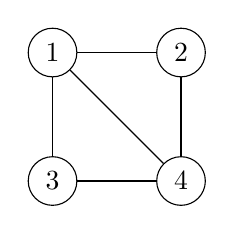
\begin{tikzpicture}[every node/.style={circle, draw, minimum size=0.30cm}]

  \node (1) {1};
  \node[right=of 1] (2) {2};
  \node[below=of 1] (3) {3};
  \node[right=of 3] (4) {4};

  \foreach \i/\j in {1/2, 1/3, 1/4, 2/4, 3/4} {
    \draw (\i) -- (\j);
  }

\end{tikzpicture}
\end{center}

We say two vertices are adjacent if there is an edge between them. For example $1$ \& $2$ are adjacent, $2$ \& $3$ are not.

We define the neighbours of a vertex to be all the vertices that it is adjacent to.

\underline{Example} 

The neighbours of $2$ are $1$ \& $4$

If we can draw the graph in such a way that no edges cross each other, then that graph is called planar. The previous example is planar. 

\underline{Example}

The graph $G$ on five vertices, and an edge between every pair of vertices is not planar. 

\begin{center}
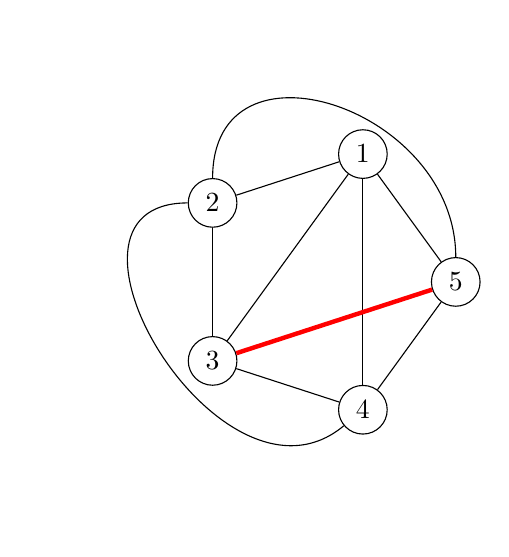
\begin{tikzpicture}[node distance=0.4cm, every node/.style={circle, draw, minimum size=0.30cm}, scale=0.03cm]

  \foreach \i in {1,...,5} {
    \node (\i) at ({\i*360/5}:2) {\i};
  }

  \draw (1) -- (3);
  \draw (1) -- (4);
  \draw[red, ultra thick](3) -- (5);
  \draw (5) -- (1);
  \draw (1) -- (2);
  \draw (3) -- (4);
  \draw (4) -- (5);
  \draw (2) -- (3);
  \draw (2) to[out=90, in=-270, looseness=1.5] (5);
  \draw (2) to[out=180, in=220, looseness=1.5] (4);
\end{tikzpicture}
\end{center}

In this case, if we remove any edge, the new graph is planar. 

\begin{center}
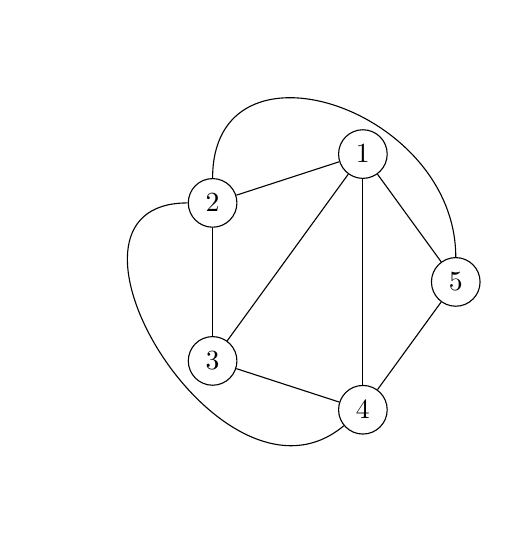
\begin{tikzpicture}[node distance=0.4cm, every node/.style={circle, draw, minimum size=0.30cm},scale=0.03cm]

  \foreach \i in {1,...,5} {
    \node (\i) at ({\i*360/5}:2) {\i};
  }

  \draw (1) -- (3);
  \draw (1) -- (4);
  \draw (5) -- (1);
  \draw (1) -- (2);
  \draw (3) -- (4);
  \draw (4) -- (5);
  \draw (2) -- (3);
  \draw (2) to[out=90, in=-270, looseness=1.5] (5);
  \draw (2) to[out=180, in=220, looseness=1.5] (4);

\end{tikzpicture}
\end{center}

There are a huge number of applications to graph theory.

\begin{enumerate}
    \item Networks
    \item Traveling Salesperson Problem
    \item Colouring countries on a map
\end{enumerate}

There are a lot of variations (which are all interesting)
\begin{enumerate}
    \item Multiple edges
    \item Loops
    \item Directions
    \item Weights
    \item Infinite graphs
    \item We could allow unordered types (instead of pairs)
\end{enumerate}

\underline{Definition}

We say that the degree of a vertex $\deg(v)$ is the number of edges touching the vertex.

\begin{center}
\begin{tikzpicture}[node distance=1cm, every node/.style={circle, draw, minimum size=0.30cm}]

  \foreach \i in {1,...,5} {
    \node (\i) at ({\i*360/5}:2) {\i};
  }

  \draw (1) -- (3);
  \draw (1) -- (4);
  \draw (5) -- (1);
  \draw (1) -- (2);
  \draw (3) -- (4);
  \draw (4) -- (5);
  \draw (2) -- (3);
  \draw (2) to[out=90, in=-270, looseness=2] (5);
  \draw (2) to[out=180, in=220, looseness=1.7] (4);
  
  \node [draw=none, above left=of 2, align=center] (6) {deg 4};
  \node[draw=none, left=of 3, align=center] (7) {deg 3};
  \draw [->] (6) -- (2);
  \draw [->] (7) -- (3);
\end{tikzpicture}
\end{center}

\underline{Fact}

The degree of $v$ is equal to the number of neighbours of $v$.

\underline{Proof}

At the other edge of an edge touching $v$ is a neighbour of $v$. 


\underline{Theorem}

\begin{align*}
    \sum_{v \in V(G)}\deg(v) = 2 |E(G)|
\end{align*}    
\underline{Proof}

We see each edge is connected to two vertices, say $v_1$ \& $v_2$. Hence each edge contributes $1$ to the degree of $v_1$ and $1$ to the degree of $v_2$. This gives the equation. 

\underline{Corollary}

The number of vertices with odd degree is even.

Recall that we showed

$\sum_{v \in V(G)}\deg(v) = 2|E(G)|$

The right hand side is an even number.

Hence $\sum_{v \in V(G)}\deg(v)$ must be even.

If we had an odd number of vertices of odd degree, then $\sum_{v \in V(G)}\deg(v)$ would be odd.

Hence we have an even number of vertices of odd degree.

\underline{Corollary}

The average degree of a vertex is

\begin{align*}
    \frac{2|E(G)|}{|V(G)|}
\end{align*}
\underline{Proof}

Average degree
\begin{align*}
    \frac{1}{|V(G)|} \sum_{v \in V(G)}\deg(v) = \frac{2|E(G)|}{|V(G)|}
\end{align*}


\subsection{Isomorphism}

\underline{Definition}

Let $G_1$ and $G_2$ be graphs. We say $G_1$ is isomorphic to $G_2$ ($G_1 \simeq G_2$) if there exists a bijection $f: V(G_1) \to V(G_2)$ with the additional property that

\begin{align*}
    (v_1, v_2) \in E(G_1) \iff (f(v_1),f(v_2)) \in E(G_2)
\end{align*}

\underline{Example}

\begin{center}
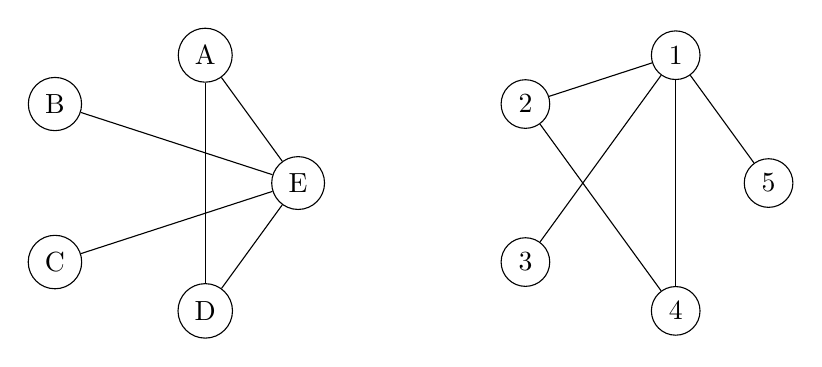
\begin{tikzpicture}[node distance=0.8cm, every node/.style={circle, draw, minimum size=0.30cm}, scale=0.03cm]

\foreach \i/\letter in {1/A, 2/B, 3/C, 4/D, 5/E} {
    \node (\i) at ({\i*360/5}:2) {\letter};
  }

  \draw (1) -- (5);
  \draw (1) -- (4);
  \draw (5) -- (2);
  \draw (5) -- (3);
  \draw (5) -- (4);

    \begin{scope}[xshift=7cm]
        \foreach \i/\letter in {1,2,3,4,5} {
    \node (\i) at ({\i*360/5}:2) {\letter};
  }

  \draw (1) -- (5);
  \draw (1) -- (4);
  \draw (1) -- (2);
  \draw (1) -- (3);
  \draw (2) -- (4);

    \end{scope}

\end{tikzpicture}
\end{center}

To see these are isomorphic, consider the bijection

\begin{align*}
    A \longrightarrow 4 \\
    B \longrightarrow 3 \\
    C \longrightarrow 5 \\
    D \longrightarrow 2 \\ 
    E \longrightarrow 1
\end{align*}


This is easy to see there is a bijection from $V(G_1)$ to $V(G_2)$


We can check the edges

\begin{align*}
    E(G_1) &\longrightarrow E(G_2) \\
    (A,D) &\longrightarrow (4,2) \\
    (E,A) &\longrightarrow (1,4) \\
    (E,B) &\longrightarrow (1,3) \\
    (E,C) &\longrightarrow (1,5) \\
    (E,B) &\longrightarrow (1,2)
\end{align*}


\underline{Fact}

Let $G_1$ and $G_2$ be isomorphic with bijection $f: V(G_1) \to V(G_2)$.

Then
\begin{enumerate}
    \item They have the same number of vertices
    \item Same number of edges
    \item $\deg(v) = \deg(f(v))$
\end{enumerate}

\begin{center}
\begin{tikzpicture}[node distance=1cm, every node/.style={circle, draw, minimum size=0.30cm}]

    \node[fill=none] (1) {};
    \node[fill=none, below left=of 1] (2) {};
    \node[fill=none, below right=of 1] (3) {};
    \node[fill=none, below=of 1] (4) {};

    \draw (1) -- (2);
    \draw (1) -- (3);
    \draw (2) -- (4);
    \draw (3) -- (4);
    \draw (2) -- (3);

    \node[draw=none, above=1cm] at (1) {$G_1$};

    
    \begin{scope}[xshift=7cm]
         for the second graph
        \node[] (5) {};
        \node[below left=of 5] (6) {};
        \node[below right=of 5] (7) {};
        \node[right=of 5] (8) {};

        \draw (5) -- (6);
        \draw (5) -- (7);
        \draw (5) -- (8);
        \draw (6) -- (7);

        \node[draw=none, above=1cm] at (5) {$G_2$};
    \end{scope}

\end{tikzpicture}
\end{center}

\begin{center}
\begin{tikzpicture}[node distance=1cm, every node/.style={circle, draw, minimum size=0.30cm}]

    
    \node[fill=none] (1) {};
    \node[fill=none, below left=of 1] (2) {};
    \node[fill=none, below right=of 2] (3) {};
    \node[fill=none, right=of 3] (4) {};
    \node[fill=none, right=of 1](5) {};

    \draw (1) -- (2);
    \draw (1) -- (3);
    \draw (1) -- (5);
    \draw (3) -- (4);
    \draw (2) -- (3);

    \node[draw=none, above=1cm] at (1) {$G_3$};

    
    \begin{scope}[xshift=5cm]
        
    \node[fill=none] (6) {};
    \node[fill=none, below left=of 6] (7) {};
    \node[fill=none, below right=of 6] (8) {};
    \node[fill=none, below=of 6] (9) {};

    \draw (6) -- (7);
    \draw (6) -- (8);
    \draw (7) -- (8);
    \draw (6) -- (9);
        \node[draw=none, above=1cm] at (6) {$G_4$};
    \end{scope}
    
    
    \begin{scope}[xshift=10cm]

    \node[fill=none] (10) {};
    \node[fill=none, below left=of 10] (11) {};
    \node[fill=none, below right=of 10] (12) {};
    \node[fill=none, below=of 10] (13) {};

    \draw (10) -- (11);
    \draw (10) -- (12);
    \draw (11) -- (13);
    \draw (13) -- (12);

    \node[draw=none, above=1cm] at (10) {$G_5$};

    \end{scope}

\end{tikzpicture}
\end{center}

Which are isomorphic? Which are not?


\begin{table}[h!]
    \begin{tabular}{|c|c|c|c|c|c|} \hline 
         &  $G_1$&  $G_2$&  $G_3$&  $G_4$& $G_5$\\ \hline 
         Edges&  5&  4&  5&  4& 4\\ \hline 
         Vertices&  4&  4&  5&  4& 4\\ \hline 
         $\#$ of vertices with deg 1&  0&  1&  2&  1& 0\\ \hline
    \end{tabular}
    \label{tab:my_label}
\end{table}


Based on this information, the only two graphs that \underline{might} be isomorphic are $G_2$ and $G_4$.


\underline{Example}

\begin{center}
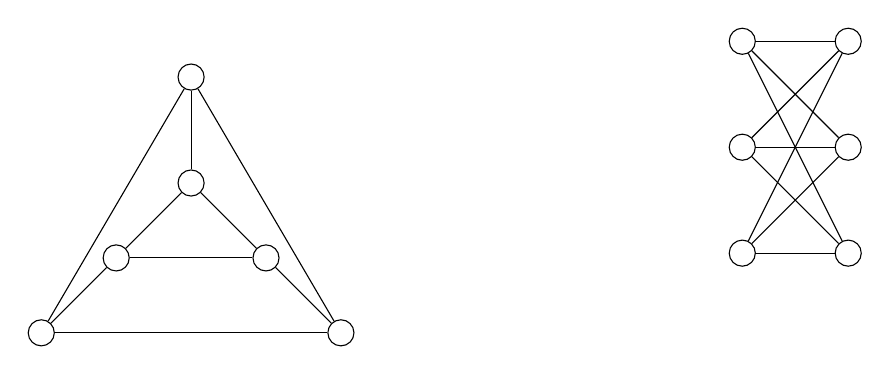
\begin{tikzpicture}[node distance=1cm, every node/.style={circle, draw, minimum size=0.30cm}]

    \node[fill=none] (1) {};
    \node[fill=none, below left=of 1] (2) {};
    \node[fill=none, below right=of 1] (3) {};
    \node[fill=none, above=of 1] (4) {};
    \node[fill=none, below left=of 2] (5) {};
    \node[fill=none, below right=of 3] (6) {};

    \draw (1) -- (4);
    \draw (1) -- (2);
    \draw (1) -- (3);
    \draw (4) -- (5);
    \draw (4) -- (6);
    \draw (5) -- (2);
    \draw (6) -- (3);
    \draw (5) -- (6);
    \draw (2) -- (3);


    
    \begin{scope}[xshift=7cm, yshift=1.8cm]
        \node[] (5) {};
        \node[below=of 5] (6) {};
        \node [below=of 6] (7) {};
        \node [right=of 5] (8) {};
        \node [below=of 8] (9) {};
        \node [below=of 9] (10) {};
        
        \draw (5) -- (8);
        \draw (6) -- (8);
        \draw (7) -- (8);
        \draw (5) -- (9);
        \draw (6) -- (9);
        \draw (7) -- (9);
        \draw (5) -- (10);
        \draw (6) -- (10);
        \draw (7) -- (10);

    \end{scope}

\end{tikzpicture}
\end{center}

These are not isomorphic despite having the same number of edges, vertices, and all vertices having the same degree (3). 


\underline{Definition}

We say a graph is $k-$regular if $\deg(v) =k$ for all $v \in V(G)$.

We say a graph is regular if it is $k-$regular for some $k$. 

\underline{Example}

The graph with $1$ vertex and no edges is $0-$regular.

The graph with $n$ vertices and no edges is $0-$regular.

\underline{Example}

What do the $1-$regular graphs look like?

\begin{center}
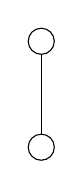
\begin{tikzpicture}[node distance=1cm, every node/.style={circle, draw, minimum size=0.30cm}]

  \node[] (1) {};
  \node [below=of 1] (2) {};
  \draw (1) -- (2);

\end{tikzpicture}
\end{center}

1-regular graph with 2 vertices.

As the number of vertices of odd degree is even, and 1 is odd, we have that 1-regular graphs have an even number of vertices. 

\begin{center}
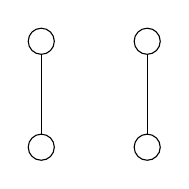
\begin{tikzpicture}[node distance=1cm, every node/.style={circle, draw, minimum size=0.30cm}]

  \node[] (1) {};
  \node [below=of 1] (2) {};
  \node [right=of 1] (3) {};
  \node [below=of 3] (4) {};
  \draw (1) -- (2);
  \draw (3) -- (4);

\end{tikzpicture}
\end{center}

1 regular graph with 4 vertices.

In general, a 1 regular graph looks like

\begin{center}
\begin{tikzpicture}[node distance=1cm, every node/.style={circle, draw, minimum size=0.30cm}]

  \node[] (1) {};
  \node [below=of 1] (2) {};
  \node [right=of 1] (3) {};
  \node [below=of 3] (4) {};
  \draw (1) -- (2);
  \draw (3) -- (4);
  \node[draw=none, right=of 4] (7) {$\cdots$};
  \node [right=of 7] (5) {};
  \node [above=of 5] (6) {};
  \draw (5) -- (6);
\end{tikzpicture}
\end{center}

\underline{Example}

What do 2-regular graphs look like?


\begin{center}
\begin{tikzpicture}[node distance=1cm, every node/.style={circle, draw, minimum size=0.30cm}]

    \node[fill=none] (1) {};
    \node[fill=none, below left=of 1] (2) {};
    \node[fill=none, below right=of 1] (3) {};

    \draw (1) -- (2);
    \draw (1) -- (3);
    \draw (2) -- (3);

    \begin{scope}[xshift=5cm]
    \node[fill=none] (6) {};
    \node[below left=of 6] (7) {};
    \node [below=of 7] (8) {};
    \node [below right=of 8] (9) {};
    \node [right=of 9] (10) {};
    \node [above right=of 10] (11) {};
    \node [above=of 11] (12) {};
    \node [above left=of 12] (13) {};
    \draw (6) -- (7);
    \draw (7) -- (8);
    \draw (8) -- (9);
    \draw (9) -- (10);
    \draw (10) -- (11);
    \draw (11) -- (12);
    \draw (12) -- (13);
    \draw (13) -- (6);

    
    \end{scope}
      
\end{tikzpicture}

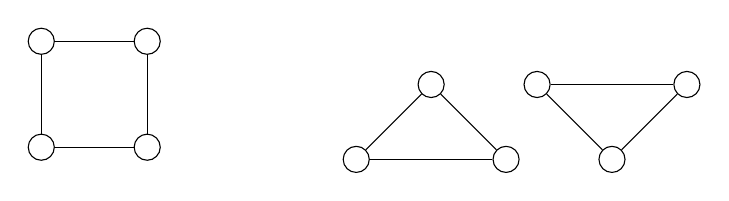
\begin{tikzpicture}[node distance=1cm, every node/.style={circle, draw, minimum size=0.30cm}]

    \node[fill=none] (1) {};
    \node[fill=none, below=of 1] (2) {};
    \node[fill=none, right=of 1] (3) {};
    \node[below=of 3] (4) {};

    \draw (1) -- (2);
    \draw (1) -- (3);
    \draw (3) -- (4);
    \draw (2) -- (4);

    
    \begin{scope}[xshift=4cm, yshift=-1.5cm]
    \node[fill=none] (6) {};
    \node[above right=of 6] (7) {};
    \node [below right=of 7] (8) {};
    \node [right=of 8] (11) {};
    \node [above left=of 11] (9) {};
    \node [above right=of 11] (10) {};
    \draw (6) -- (7);
    \draw (6) -- (8);
    \draw (7) -- (8);
    \draw (9) -- (10);
    \draw (9) -- (11);
    \draw (10) -- (11);
    
    \end{scope}
    
\end{tikzpicture}
\end{center}

2 regular graphs are a collection of disjoint cycles. 

\underline{Example}

What is the smallest $k-$regular graph (i.e. minimal vertices)?

\underline{k+1}

Let $V(G) = \{1,2,\ldots, k+1\}$ and put an edge between every pair of vertices. 

\underline{Definition}

A complete graph $\mathcal{K}_n$ is a graph with $n-$vertices and an edge between every vertex. 

\underline{Note} $\mathcal{K}$ is $(n-1)-$regular


\begin{center}
\begin{tikzpicture}[node distance=1cm, every node/.style={circle, draw, minimum size=0.30cm}]

  \node[] (1) {};
  \node [right=of 1] (3) {};
  \node [below=of 3] (4) {};
  \draw (3) -- (4);

  \node[right=of 4] (5) {};
  \node [above right=of 5] (6) {};
  \node [below right=of 6] (7) {};
  \draw (5) -- (6);
  \draw (6) -- (7);
  \draw (5) -- (7);

  \node [right=of 7] (8) {};
  \node [above right =of 8] (10) {};
  \node [above=of 10] (9) {};
  \node [below right =of 10] (11) {};
  \draw (8) -- (9);
  \draw (8) -- (10);
  \draw (8) -- (11);
  \draw (9) -- (10);
  \draw (9) -- (11);
  \draw (10)--(11);
  \node[right=of 11, draw=none] (ellipsis1) at (9,-1) {$\cdots$};


\end{tikzpicture}
\end{center}


\underline{Question}

How many edges does $\mathcal{K}_n$ have?

We know there are $n-$vertices, and every vertex has degree $n-1$.

This gives

\begin{align*}
    2 |E(G)| = \sum_{v \in V(G)}\deg(v) &= \sum_{v \in V(G)} n-1 \\
    &= n \cdot (n-1)  \\
    \implies |E(G)| = \frac{n(n-1)}{2}
\end{align*}

\subsection{Bipartite Graphs}

\underline{Definition}

We say $G$ is a bipartite graph if we can divide the vertices $V(G)$ into two disjoint sets $A$ and $B$ such that all edges have one end in $A$ and one end in $B$.

\underline{Example}

Which of the following are bipartite ($G_1$, $G_2$, $G_3$ respectively)?

\begin{center}
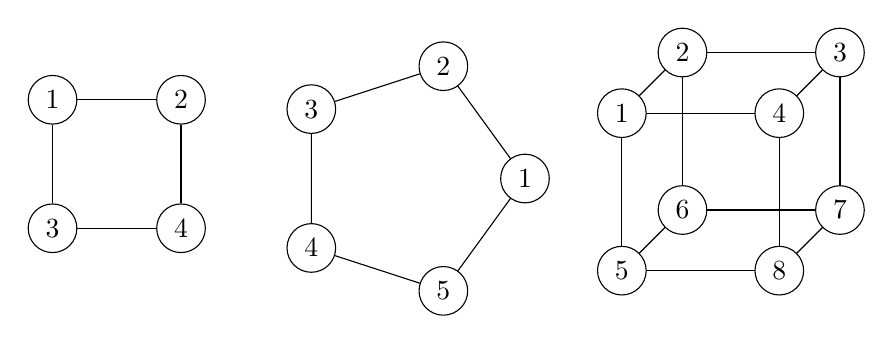
\begin{tikzpicture}[node distance=1cm, every node/.style={circle, draw, minimum size=0.30cm}]

  \node (1) {1};
  \node[right=of 1] (2) {2};
  \node[below=of 1] (3) {3};
  \node[right=of 3] (4) {4};

  \foreach \i/\j in {1/2, 1/3, 2/4, 3/4} {
    \draw (\i) -- (\j);
  }

  \begin{scope}[xshift=4.5cm, yshift=-1cm]
        
    \def\radius{1.5cm}
    
    \foreach \i in {1,...,5} {
        \coordinate (P\i) at ({360/5 * (\i - 1)}:\radius);
    }
    
    \draw (P1) -- (P2) -- (P3) -- (P4) -- (P5) -- cycle;
    
    \foreach \i in {1,...,5} {
        \node at (P\i) [circle, draw, fill=white] {\i};
    }
    
    \end{scope}

    \begin{scope}[xshift=8cm,scale=2,yshift=-0.7cm]
    
    \coordinate (A) at (0,0,0);
    \coordinate (B) at (1,0,0);
    \coordinate (C) at (1,1,0);
    \coordinate (D) at (0,1,0);
    \coordinate (E) at (0,0,1);
    \coordinate (F) at (1,0,1);
    \coordinate (G) at (1,1,1);
    \coordinate (H) at (0,1,1);
    
    \draw (A) -- (B) -- (C) -- (D) -- cycle;
    \draw (E) -- (F) -- (G) -- (H) -- cycle;
    \draw (A) -- (E);
    \draw (B) -- (F);
    \draw (C) -- (G);
    \draw (D) -- (H);
    
    \foreach \i/\name in {A/6, B/7, C/3, D/2, E/5, F/8, G/4, H/1} {
        \node at (\i) [circle, draw, fill=white] {\name};
    }
    
    \end{scope}
\end{tikzpicture}
\end{center}


$G_1$ is bipartite. To see this, let $A=\{1,4\}$ and $B=\{2,3\}$

\begin{center}
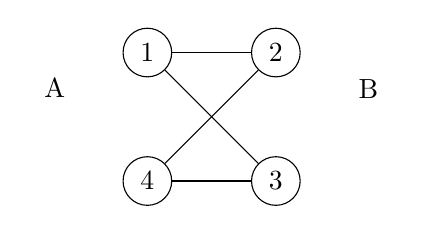
\begin{tikzpicture}[node distance=1cm, every node/.style={circle, draw, minimum size=0.30cm}]

  \node (1) {1};
  \node[right=of 1] (2) {2};
  \node[below=of 2] (3) {3};
  \node[below=of 1] (4) {4};
  \node[draw=none, above left=of 4] (5) {A};
  \node[draw=none, above right=of 3] (6) {B};

  \foreach \i/\j in {1/2, 1/3, 2/4, 3/4} {
    \draw (\i) -- (\j);
  }

\end{tikzpicture}
\end{center}

$G_2$ is not bipartite. To see this, assume it is, and hope for a contradiction. Assume without loss of generality that $1 \in A$. As there is an edge from $1$ to $5$ and $1$ to $2$, as there are no edges from $A$ to $A$, we see $2,5 \in B$. There is an edge from $5$ to $4$, hence $4 \in A$. Similarly, there is an edge between $2$ and $3$. Hence, $3 \in A$. But there is an edge from 3 to 4, both in $A$. 

This gives us a contradiction. Hence $G_2$ is not bipartite. 

For $G_3$ we can assume a vertex is in $A$, and see what we derive. 


\begin{center}
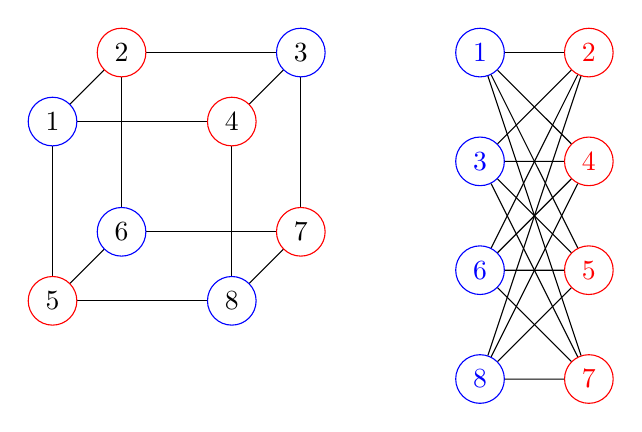
\begin{tikzpicture}[node distance=0.75cm, every node/.style={circle, draw, minimum size=0.30cm}, scale=0.08cm]

    \coordinate (A) at (0,0,0);
    \coordinate (B) at (1,0,0);
    \coordinate (C) at (1,1,0);
    \coordinate (D) at (0,1,0);
    \coordinate (E) at (0,0,1);
    \coordinate (F) at (1,0,1);
    \coordinate (G) at (1,1,1);
    \coordinate (H) at (0,1,1);
    
    \draw (A) -- (B) -- (C) -- (D) -- cycle;
    \draw (E) -- (F) -- (G) -- (H) -- cycle;
    \draw (A) -- (E);
    \draw (B) -- (F);
    \draw (C) -- (G);
    \draw (D) -- (H);
    
    \foreach \i/\name\color in {A/6/blue, B/7/red, C/3/blue, D/2/red, E/5/red, F/8/blue, G/4/red, H/1/blue} {
        \node at (\i) [circle, draw=\color, fill=white] {\name};
    }

    \begin{scope}[xshift=2cm,yshift=1cm]
        \node[color=blue,] (5) {1};
        \node[color=blue,below=of 5] (6) {3};
        \node [color=blue,below=of 6] (7) {6};
        \node [color=blue,below=of 7] (11) {8};
        \node [color=red,right=of 5] (8) {2};
        \node [color=red,below=of 8] (9) {4};
        \node [color=red,below=of 9] (10) {5};
        \node [color=red,below=of 10] (12) {7};
        
        \draw (5) -- (8);
        \draw (6) -- (8);
        \draw (7) -- (8);
        \draw (5) -- (9);
        \draw (6) -- (9);
        \draw (7) -- (9);
        \draw (5) -- (10);
        \draw (6) -- (10);
        \draw (7) -- (10);
        \draw (11) -- (8);
        \draw (11) -- (9);
        \draw (11) -- (10);
        \draw (12) -- (5);
        \draw (12) -- (6);
        \draw (12) -- (7);
        \draw (12) -- (11);

    \end{scope}  
    

\end{tikzpicture}
\end{center}

\underline{Example}

Let $G$ be a 1-regular graph on 10 vertices. 

\begin{center}
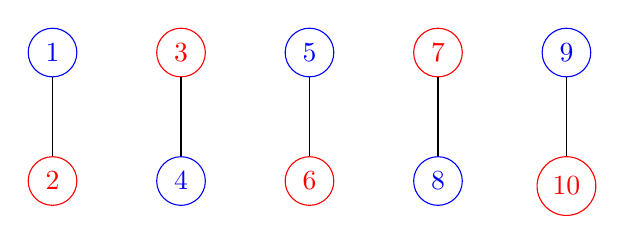
\begin{tikzpicture}[node distance=1cm, every node/.style={circle, draw, minimum size=0.30cm}]

  \node[color=blue] (1) {1};
  \node [color=red, below=of 1] (2) {2};
  \node [color=red,right=of 1] (3) {3};
  \node [color=blue,below=of 3] (4) {4};
  \node [color=blue,right=of 3] (5) {5};
  \node [color=red,below=of 5] (6) {6};
  \node [color=red,right=of 5] (7) {7};
  \node [color=blue,below=of 7] (8) {8};
  \node [color=blue,right=of 7] (9) {9};
  \node [color=red,below=of 9] (10) {10};
  \draw (1) -- (2);
  \draw (3) -- (4);
  \draw (5) -- (6);
  \draw (7) -- (8);
  \draw (9) -- (10);

\end{tikzpicture}
\end{center}

This is bipartite. To see this, we could set $A = \{1,3,5,7,9\}, B = \{2,4,6,8,10\}$

\underline{OR}

$A = \{1,4,5,8,9\}, B = \{2,3,6,7,10\}$


\underline{Example}

Let $G$ be a graph on 100 vertices, $V(G) = \{1,2,3,\ldots, 100\}$

We say $(v_1, v_2) \in E(G)$ if and only if $|v_1 - v_2| = 1$ or $|v_1 - v_2| = 3$

The first couple vertices of this graph are 

\begin{center}
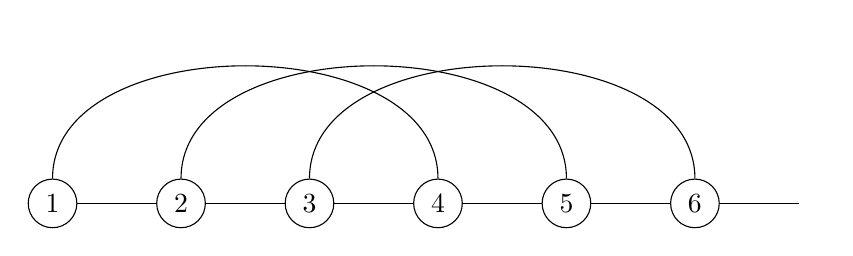
\begin{tikzpicture}[node distance=1cm, every node/.style={circle, draw, minimum size=0.30cm}]

  \node[] (1) {1};
  \node [right=of 1] (2) {2};
  \node [right=of 2] (3) {3};
  \node [right=of 3] (4) {4};
  \node [right=of 4] (5) {5};
  \node [right=of 5] (6) {6};
  \node [draw=none, right=of 6] (7) {};
  \draw (1) -- (2);
  \draw (3) -- (4);
  \draw (2) -- (3);
  \draw (4) -- (5);
  \draw (5) -- (6);
  \draw (6) -- (7);
  \draw (1) to[out=90, in=90] (4);
  \draw (2) to[out=90, in=90] (5);
  \draw (3) to[out=90,in=90] (6);

\end{tikzpicture}
\end{center}

We see that odd numbers are not connected to each other, and even numbers are not connected to each other. We can take 

$A = \{1,3,5,\ldots,99\} B = \{2,4,6,\ldots,100\}$

\underline{Note}

Technically "connected" has meaning in graph theory. It is better to say there is no edge between two odd vertices. 

\underline{Definition}

We say $G$ is a complete bipartite graph if it is bipartite, and every vertex in $A$ has an edge to every vertex in $B$. 

This is typically denoted $\mathcal{K}_{n,m}$ where $|A| = n, |B| = m$.

$\mathcal{K}_{2,2}, \mathcal{K}_{2,3}, \mathcal{K}_{3,3}$ respectively.

\begin{center}
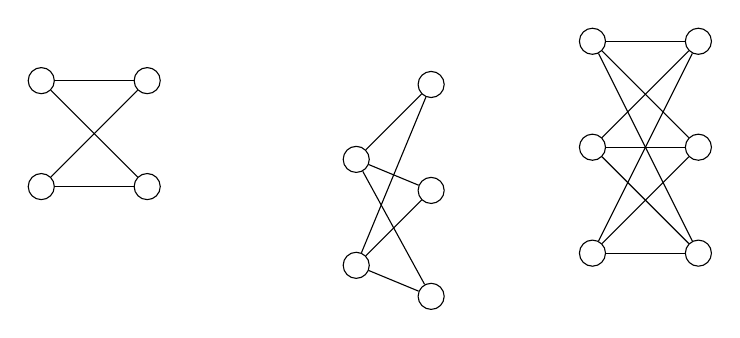
\begin{tikzpicture}[node distance=1cm, every node/.style={circle, draw, minimum size=0.30cm}]

  \node (1) {};
  \node[right=of 1] (2) {};
  \node[below=of 2] (3) {};
  \node[below=of 1] (4) {};

  \foreach \i/\j in {1/2, 1/3, 2/4, 3/4} {
    \draw (\i) -- (\j);
  }

    \begin{scope}[xshift=4cm,yshift=-1cm]
    \node[] (6) {};
    \node[below=of 6] (7) {};
    \node[above right=of 6] (8) {};
    \node [below =of 8] (9) {};
    \node [below=of 9] (10) {};

    \draw (6) -- (8);
    \draw (6) -- (9);
    \draw (6) -- (10);
    \draw (7) -- (8);
    \draw (7) -- (9);
    \draw (7) -- (10);
    \end{scope}

    \begin{scope}[xshift=7cm, yshift=0.5cm]
        \node[] (12) {};
        \node[below=of 12] (13) {};
        \node [below=of 13] (14) {};
        \node [right=of 12] (15) {};
        \node [below=of 15] (16) {};
        \node [below=of 16] (17) {};
        
        \draw (12) -- (15);
        \draw (13) -- (15);
        \draw (14) -- (15);
        \draw (12) -- (16);
        \draw (13) -- (16);
        \draw (14) -- (16);
        \draw (12) -- (17);
        \draw (13) -- (17);
        \draw (14) -- (17);

    \end{scope}
    
\end{tikzpicture}
\end{center}
%^graph

\underline{Question}

How many vertices does $\mathcal{K}_{n,m}$ have? 

We see $n = |A|, m = |B|$ and $V(G)$ is a disjoint union of $A$ and $B$. So $|V(G)| = m + n$.

The number of edges is $m \cdot n$. To see this, note that there are $n$ vertices in $A$. Further, every vertex has an edge to all $m$ vertices in $B$. There are no other edges. Hence there are $n \cdot m$ edges. 

\underline{Theorem}

Let $G_1$ be isomorphic to $G_2$. Then $G_1$ is bipartite $\iff G_2$ is bipartite. 

\underline{Proof}

To see this, let $f: V(G_1) \to V(G_2)$ be an edge-preserving bijection. Then if $A, B$ demonstrate $G_1$ is bipartite, $f(A), f(B)$ will demonstrate $G_2$ is bipartite. 

\underline{Example}

Consider the 3-regular graphs on 6-vertices.

\begin{center}
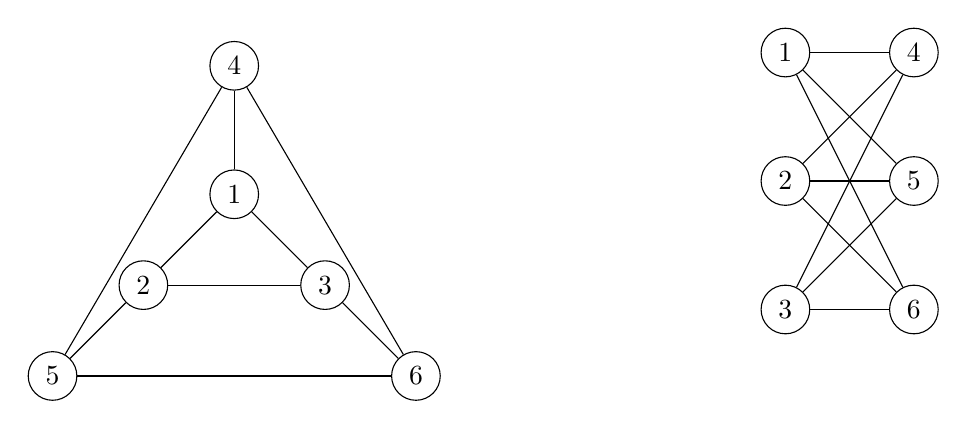
\begin{tikzpicture}[node distance=1cm, every node/.style={circle, draw, minimum size=0.30cm}]


    \node[fill=none] (1) {1};
    \node[fill=none, below left=of 1] (2) {2};
    \node[fill=none, below right=of 1] (3) {3};
    \node[fill=none, above=of 1] (4) {4};
    \node[fill=none, below left=of 2] (5) {5};
    \node[fill=none, below right=of 3] (6) {6};


    \draw (1) -- (4);
    \draw (1) -- (2);
    \draw (1) -- (3);
    \draw (4) -- (5);
    \draw (4) -- (6);
    \draw (5) -- (2);
    \draw (6) -- (3);
    \draw (5) -- (6);
    \draw (2) -- (3);



    \begin{scope}[xshift=7cm, yshift=1.8cm]
        \node[] (5) {1};
        \node[below=of 5] (6) {2};
        \node [below=of 6] (7) {3};
        \node [right=of 5] (8) {4};
        \node [below=of 8] (9) {5};
        \node [below=of 9] (10) {6};
        
        \draw (5) -- (8);
        \draw (6) -- (8);
        \draw (7) -- (8);
        \draw (5) -- (9);
        \draw (6) -- (9);
        \draw (7) -- (9);
        \draw (5) -- (10);
        \draw (6) -- (10);
        \draw (7) -- (10);

    \end{scope}

\end{tikzpicture}
\end{center}

We see $G_2$ is bipartite (and is isomorphic to $\mathcal{K}_{3,3}$ using $A = \{1,2,3\}, B = \{4,5,6\}$).

$G_1$ is \underline{not} bipartite. To see this, assume $1 \in A$. Then $2,3 \in B$. But there is an edge from 2 to 3. A contradiction. 

\underline{Example}

Let $\mathcal{K}_{n,m}$ be a $k-$regular bipartite graph. Show $n=m$ or $k = 0$.


If $\mathcal{K}_{n,m}$ is $k-$regular, we see every vertex in $A$ has degree $k$.

So there are $k \cdot n$ edges. 

Similarly, looking at $B$, we have $k \cdot m$ edges. 

This gives $kn = km$, hence $k = 0$ or $m = n$.

\subsection{Specifying Graphs}

1) Draw a picture

\begin{center}
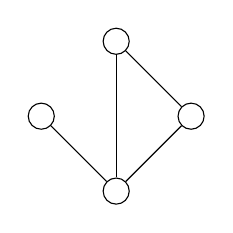
\begin{tikzpicture}[node distance=1cm, every node/.style={circle, draw, minimum size=0.30cm}]

    \node[fill=none] (1) {};
    \node[fill=none, below left=of 1] (2) {};
    \node[fill=none, below right=of 1] (3) {};
    \node[fill=none, below right=of 2] (4) {};

    \draw (1) -- (4);
    \draw (1) -- (3);
    \draw (3) -- (4);
    \draw (2) -- (4);
\end{tikzpicture}
\end{center}

2) Specify the vertices and edges.

$V(G) = \{1,2,3\}$

$E(G) = \{(1,2),(1,3)\}$

3) Giving the vertices, and a rule for the edges.

\underline{Example}

Let $V(G)$ be the set of all subsets of $\{1,2,3\}$

We say $(A,B) \in E(G)$ if $A \cap B = \emptyset$

\begin{center}
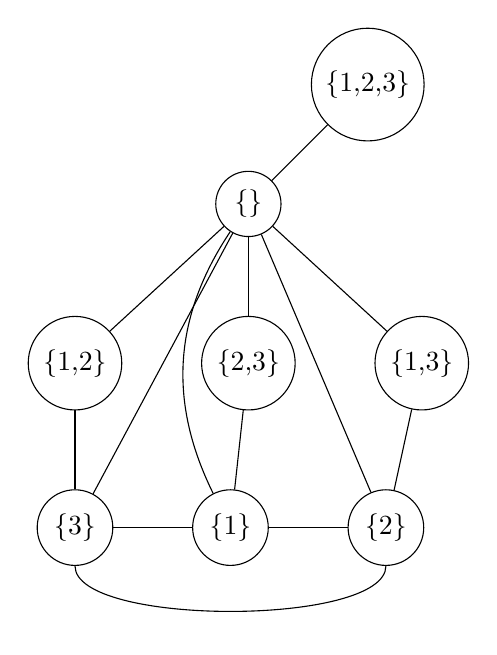
\begin{tikzpicture}[node distance=1cm, every node/.style={circle, draw, minimum size=0.30cm}]

    \node[fill=none] (1) {\{\}};
    \node[fill=none, above right=of 1] (2) {\{1,2,3\}};
    \node[fill=none, below =of 1] (3) {\{2,3\}};
    \node[fill=none, left=of 3] (4) {\{1,2\}};
    \node[fill=none, right=of 3] (5) {\{1,3\}};
    \node[fill=none, below=of 4] (6) {\{3\}};
    \node[fill=none, right=of 6] (7) {\{1\}};
    \node[fill=none, right=of 7] (8) {\{2\}};


    \draw (1) -- (2);
    \draw (1) -- (3);
    \draw (1) -- (4);
    \draw (1) -- (5);
    \draw (1) -- (6);
    \draw (1) to[bend right] (7);
    \draw (1) -- (8);
    \draw (4) -- (6);
    \draw (3) -- (7);
    \draw (5) -- (8);
    \draw (6) -- (7);
    \draw (7) -- (8);
    \draw (6) to[out=270, in=270, looseness=0.5] (8);
\end{tikzpicture}
\end{center}

\underline{Adjacency Matrix}

This is a $|V(G)| \times |V(G)|$ matrix, with columns/rows induced by $V(G)$.

We set $M[i,j] = 1$ if $(i,j) \in E(G)$ and 0 otherwise.

\underline{Example}

\begin{center}
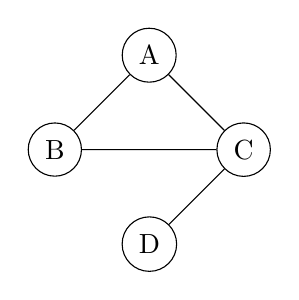
\begin{tikzpicture}[node distance=1cm, every node/.style={circle, draw, minimum size=0.30cm}]

    \node[fill=none] (1) {A};
    \node[fill=none, below left=of 1] (2) {B};
    \node[fill=none, below right=of 1] (3) {C};
    \node[fill=none, below right=of 2] (4) {D};

    \draw (1) -- (2);
    \draw (1) -- (3);
    \draw (3) -- (2);
    \draw (3) -- (4);
\end{tikzpicture}

$\begin{bmatrix}
0 & 1 & 1 & 0\\
1 & 0 & 1 & 0\\
1 & 1 & 0 & 1\\
0 & 0 & 1 & 0\\
\end{bmatrix}$
\end{center}

As there are no loops, all terms on the diagonal are 0. As the graph is undirected, $M = M^\top$. As we do not allow multiple edges, entries are bounded by 1. 

Powers of these matrices tell us information about walks. 

This is annoying if $|V(G)|$ is large. 

\underline{Adjacency List}


\begin{table}[h]
    \centering
    \begin{tabular}{c|c}
        Vertex & Neighbours\\ \hline
         $A$& $BC$\\
         $B$& $AC$\\
         $C$& $ABD$\\
         $D$& $C$\\
    \end{tabular}
\end{table}


\subsection{Paths and Cycles}


\underline{Definition}

Let $G$ be a graph. We define a walk from $v_0$ to $v_n$ as a sequence of vertices $v_0, v_1, v_2, \ldots, v_{n-1}, v_n$ such that $(v_i, v_{i+1}) \in E(G)$ for $i = 0,1,\ldots,n-1$. This is a walk of length $n$ (as there are $n-$edges). 

\underline{Example}

Find all walks of length 2 starting at 1 of 

\begin{center}
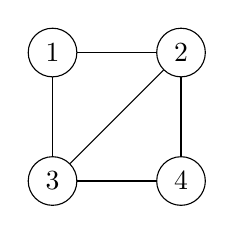
\begin{tikzpicture}[node distance=1cm, every node/.style={circle, draw, minimum size=0.30cm}]

    \node[fill=none] (1) {1};
    \node[fill=none, below =of 1] (3) {3};
    \node[fill=none,  right=of 1] (2) {2};
    \node[fill=none, below =of 2] (4) {4};

    \draw (1) -- (2);
    \draw (1) -- (3);
    \draw (3) -- (2);
    \draw (3) -- (4);
    \draw (2) -- (4);
\end{tikzpicture}
\end{center}

\begin{align*}
    1 - 3 -2 \quad 1 - 3 -1 \\
    1 - 2 -3 \quad 1 -2- 4 \\
    1-2-1 \quad 1-3-4
\end{align*}

\underline{Definition}

A path is a walk where all vertices are distinct. 

\underline{Example}

For the previous graph, there are 4 paths of length 2 starting at 1. 

They are $1-2-3, 1-3-2, 1-2-4, 1-3-4$

\underline{Fact}

The longest path in a graph $G$ has at most length $|V(G)| -1$

\underline{Example}

\begin{center}
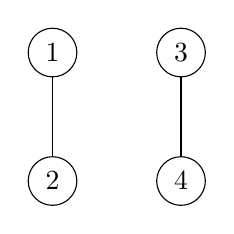
\begin{tikzpicture}[node distance=1cm, every node/.style={circle, draw, minimum size=0.30cm}]

    \node[fill=none] (1) {1};
    \node[fill=none, below =of 1] (2) {2};
    \node[fill=none,  right=of 1] (3) {3};
    \node[fill=none, below =of 3] (4) {4};

    \draw (1) -- (2);
    \draw (3) -- (4);
\end{tikzpicture}
\end{center}

The longest path is length 1, even though we have $|V(G)| = 4$

\underline{Theorem}

If there exists a walk from $x$ to $y$ then there exists a path from $x$ to $y$. 

\underline{Proof}

If $x = y$, we are done. Take the path of length 0 starting/ending at $x$.

Let $x-v_1-v_2-\ldots-v_{n-1}-y$ be a walk from $x$ to $y$. If all vertices are distinct, we are done. Hence assume $v_i = v_j$ for $i \ne j$ (with $v_0 = x, v_n = y)$. Assume $i < j$.

Consider the new walk
\begin{align*}
    x = &v_0 - v_1 - v_2 - \ldots - v_i - v_{j+1} - v_{j+2} - \ldots - v_n\\
    &\text{(Remove everything between } v_1 \text{ and } v_{j+1} \text{)}
\end{align*}

Either this new walk has all vertices distinct, or we repeat. 

Note, the initial walk is a finite length. Every time we apply this process we get something shorter. This process will eventually terminate. 

\underline{Example}

\begin{center}
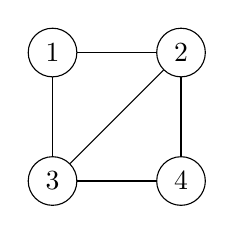
\begin{tikzpicture}[node distance=1cm, every node/.style={circle, draw, minimum size=0.30cm}]

    \node[fill=none] (1) {1};
    \node[fill=none, below =of 1] (3) {3};
    \node[fill=none,  right=of 1] (2) {2};
    \node[fill=none, below =of 2] (4) {4};

    \draw (1) -- (2);
    \draw (1) -- (3);
    \draw (3) -- (2);
    \draw (3) -- (4);
    \draw (2) -- (4);
\end{tikzpicture}
\end{center}

\begin{align*}
&1-2-3-2-4-3-2-1-3-4\\
&1-2-3-2-1-3-4\\
&1-3-4
\end{align*}
Alternatively
\begin{align*}
    &1-2-3-2-4-3-2-1-3-4 \\
    &1-2-3-4
\end{align*}

\underline{Theorem}

If there is a path from $x$ to $y$ and from $y$ to $z$ then there is a path from $x$ to $z$. 
\begin{align*}
    x-v_1-\ldots-&v_{n-1}-y-u_1-u_2-\ldots-u_{m-1}-z \\
    &\text{is a walk from } x \text{ to } z
\end{align*}

We can use the previous result to get a path. 

\underline{Definition}

Let $G_1$ and $G_2$ be graphs. 

We say $G_1$ is a subgraph of $G_2$ if $V(G_1) \subseteq V(G_2)$ and $E(G_1) \subseteq E(G_2)$.

\underline{Example}

Which of these graphs are subgraphs of another graph?

\begin{center}
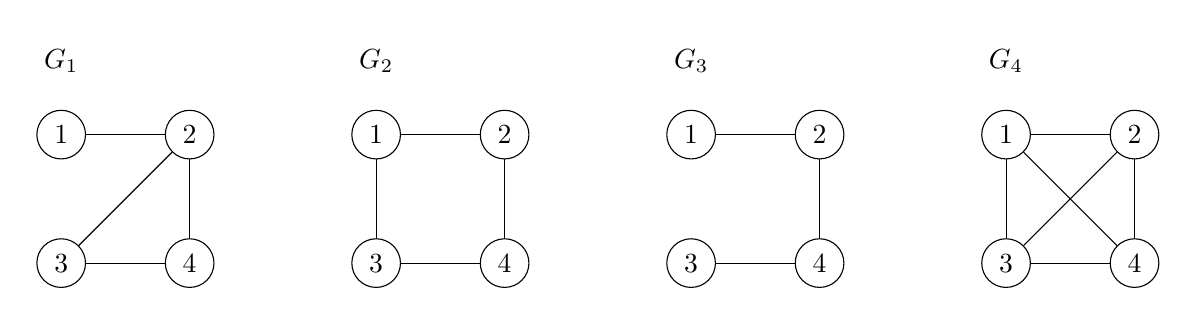
\begin{tikzpicture}[node distance=1cm, every node/.style={circle, draw, minimum size=0.30cm}]

    \node[fill=none] (1) {1};
    \node[fill=none, right=of 1] (2) {2};
    \node[fill=none, below =of 2] (4) {4};
    \node[fill=none, below=of 1] (3) {3};

    \draw (1) -- (2);
    \draw (2) -- (3);
    \draw (2) -- (4);
    \draw (3) -- (4);
    
    \node[draw=none, above=0.5cm] at (1) {$G_1$};
    \begin{scope}[xshift=4cm]
    \node[fill=none] (5) {1};
    \node[fill=none, right=of 5] (6) {2};
    \node[fill=none, below =of 6] (7) {4};
    \node[fill=none, below=of 5] (8) {3};

    \draw (5) -- (6);
    \draw (6) -- (7);
    \draw (7) -- (8);
    \draw (8) -- (5);
        \node[draw=none, above=0.5cm] at (5) {$G_2$};
    \end{scope}
    
    
    \begin{scope}[xshift=8cm]

    \node[fill=none] (9) {1};
    \node[fill=none, right=of 9] (10) {2};
    \node[fill=none, below =of 10] (11) {4};
    \node[fill=none, below=of 9] (12) {3};

    \draw (9) -- (10);
    \draw (10) -- (11);
    \draw (11) -- (12);
    

    \node[draw=none, above=0.5cm] at (9) {$G_3$};

    \end{scope}
    \begin{scope}[xshift=12cm]

    \node[fill=none] (13) {1};
    \node[fill=none, right=of 13] (14) {2};
    \node[fill=none, below =of 14] (15) {4};
    \node[fill=none, below=of 13] (16) {3};

    \draw (13) -- (14);
    \draw (14) -- (15);
    \draw (15) -- (13);
    \draw (16) -- (14);
    \draw (16) -- (13);
    \draw (16) -- (15);
    

    \node[draw=none, above=0.5cm] at (13) {$G_4$};

    \end{scope}

\end{tikzpicture}
\end{center}

$G_1, G_2, G_3,$ and $G_4$ are subgraphs of $G_4$. 

$G_3$ is a subgraph of both $G_1$ and $G_2$. 

Everything is a subgraph of itself.

\underline{Note}

Let $G_1$ be a subgraph of $G_2$ (not example above)
\begin{itemize}
    \item $|E(G_1)| \le |E(G_2)|$
    \item $|V(G_1)| \le |V(G_2)|$
    \item If $G_2$ is bipartite, then $G_1$ is (probably) bipartite. This won't work if we remove all of $A$ or all of $B$ from $V(G_2)$.
    \item Every graph $G_1$ is a subgraph of the complete graph on vertices $V(G_1)$.
\end{itemize}

\underline{Definition}

If $G_1$ is a subgraph of $G_2$ and $V(G_1) = V(G_2)$, then we say $G_1$ is a spanning subgraph of $G_2$. 

If in addition, $E(G_1) \ne E(G_2)$ then $G_1$ is a proper spanning subgraph. 

\underline{Fact}

A spanning subgraph of a bipartite graph is bipartite. 

\underline{Definition}

A connected 2-regular subgraph is called a cycle. 

\underline{Example}

Find some cycles in 

\begin{center}
\begin{tikzpicture}[node distance=1cm, every node/.style={circle, draw, minimum size=0.30cm}]

    \node[fill=none] (1) {1};
    \node[fill=none, right=of 1] (2) {2};
    \node[fill=none, below =of 2] (4) {4};
    \node[fill=none, below=of 1] (3) {3};

    \draw (1) -- (2);
    \draw (2) -- (3);
    \draw (2) -- (4);
    \draw (3) -- (4);
    \draw (1) -- (3);
    
    \node[draw=none, above=0.5cm] at (1) {$G_1$};
    \begin{scope}[xshift=4cm]
    \node[fill=none] (5) {1};
    \node[fill=none, right=of 5] (6) {2};
    \node[fill=none, below=of 5] (8) {3};

    \draw (5) -- (6);
    \draw (8) -- (5);
    \draw (8) -- (6);
    \end{scope}
    
    
    \begin{scope}[xshift=8cm]

    \node[fill=none] (9) {1};
    \node[fill=none, right=of 9] (10) {2};
    \node[fill=none, below =of 10] (11) {4};
    \node[fill=none, below=of 9] (12) {3};

    \draw (9) -- (10);
    \draw (10) -- (11);
    \draw (11) -- (12);
    \draw (9) -- (12);
    

    \end{scope}
    \begin{scope}[xshift=12cm]

    \node[fill=none, right=of 13] (14) {2};
    \node[fill=none, below =of 14] (15) {4};
    \node[fill=none, below=of 13] (16) {3};

    \draw (14) -- (15);
    \draw (16) -- (14);
    \draw (16) -- (15);
    
    \end{scope}

\end{tikzpicture}
\end{center}

\underline{Theorem}

Let $G$ be a graph such that $\deg(v) \ge 2$ for all $v \in V(G)$

Then $G$ contains a cycle. 

\underline{Proof}

Let $v_1 - v_2 - v_3 - \ldots - v_n$ be a path of maximal length. Notice, $\deg(v_n) \ge 2$.

Say $(v_n, x) \in E(G), x \ne v_{n-1}$. If $x \ne v_i$ for all $i = 1,2,\ldots, n-1$, then $v_1-v_2-v_3-\ldots-v_n-v_x$ is a longer path (which contradicts the fact that we took the longest path). 

Hence $x = v_i$ for some $i = 1,2,\ldots,n-1$

We have by assumption that $i \ne n-1$.

\begin{center}
\begin{tikzpicture}[node distance=0.5cm, every node/.style={circle, draw, minimum size=0.30cm}]
    \node[draw=none, fill=none] (1) {$v_1$};
    \node[draw=none, fill=none, right=of 1] (2) {$v_2$};
    \node[fill=none,draw=none,  right=of 2] (3) {$\ldots$};
    \node[fill=none,draw=none,  right=of 3] (4) {$v_{i-1}$};
    \node[fill=none,draw=none,  right=of 4] (5) {$v_i$};
    \node[fill=none,draw=none,  right=of 5] (6) {$v_{i+1}$};
    \node[fill=none,draw=none,  right=of 6] (7) {$\ldots$};
    \node[fill=none, draw=none, right=of 7] (8) {$v_n$};

    \draw (5) to[out=90, in=-270, looseness=0.3] (8);
    \draw (1) -- (2);
    \draw (2) -- (3);
    \draw (3) -- (4);
    \draw (4) -- (5);
    \draw (5) -- (6);
    \draw (6) -- (7);
    \draw (7) -- (8);

\end{tikzpicture}
\end{center}

This gives us a cycle $v_1-v_{i+1}-\ldots-v_n-v_i$

(Technically a walk contains more information than a cycle, as there is a concept of direction and start and end. By this we can mean the image of the walk). 

\underline{Example}

\begin{center}
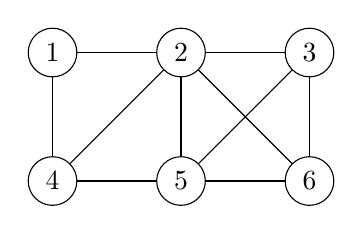
\begin{tikzpicture}[node distance=1cm, every node/.style={circle, draw, minimum size=0.30cm}]

    \node[fill=none] (1) {1};
    \node[fill=none, right =of 1] (2) {2};
    \node[fill=none,  right=of 2] (3) {3};
    \node[fill=none, below = of 1] (4) {4};
    \node[fill=none, below = of 2] (5) {5};
    \node[fill=none, below = of 3] (6) {6};
    \draw (1) -- (2);
    \draw (2) -- (3);
    \draw (2) -- (4);
    \draw (4) -- (5);
    \draw (1) -- (4);
    \draw (5) -- (6);
    \draw (6) -- (3);
    \draw (2) -- (6);
    \draw (2) -- (5);
    \draw (3) -- (5);
    
\end{tikzpicture}
\end{center}

\underline{Step 1}

Find a longest path ($1-4-2-5-3-6$). 

\begin{center}
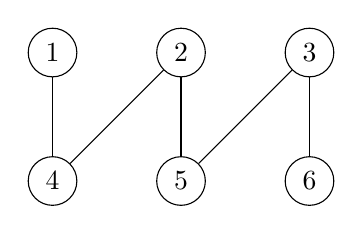
\begin{tikzpicture}[node distance=1cm, every node/.style={circle, draw, minimum size=0.30cm}]

    \node[fill=none] (1) {1};
    \node[fill=none, right =of 1] (2) {2};
    \node[fill=none,  right=of 2] (3) {3};
    \node[fill=none, below = of 1] (4) {4};
    \node[fill=none, below = of 2] (5) {5};
    \node[fill=none, below = of 3] (6) {6};
    \draw (2) -- (4);
    \draw (1) -- (4);
    \draw (6) -- (3);
    \draw (2) -- (5);
    \draw (3) -- (5);
    
\end{tikzpicture}
\end{center}

\underline{Step 2}

6 is connected to something. Say 2. 

Connect 2 to 6 and remove everything from the path before 2. 

\begin{center}
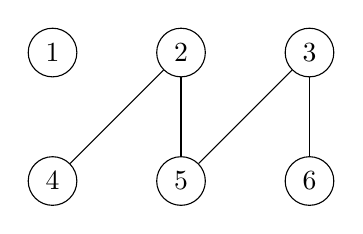
\begin{tikzpicture}[node distance=1cm, every node/.style={circle, draw, minimum size=0.30cm}]

    \node[fill=none] (1) {1};
    \node[fill=none, right =of 1] (2) {2};
    \node[fill=none,  right=of 2] (3) {3};
    \node[fill=none, below = of 1] (4) {4};
    \node[fill=none, below = of 2] (5) {5};
    \node[fill=none, below = of 3] (6) {6};
    \draw (2) -- (4);
    \draw (6) -- (3);
    \draw (2) -- (5);
    \draw (3) -- (5);
    
\end{tikzpicture}
\end{center}

Walk $2-5-3-6-2$

\underline{Definition}

We say the girth of a graph is the size of the smallest cycle. 

\underline{Definition}

We say a cycle is a Hamiltonian cycle if it contains every vertex. 

\underline{Definition}

A path is a Hamiltonian path if it visits every vertex. 

\underline{Example}

\begin{center}
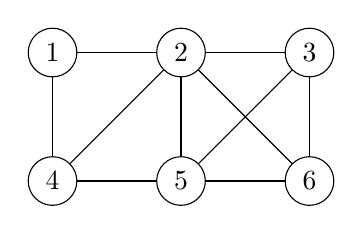
\begin{tikzpicture}[node distance=1cm, every node/.style={circle, draw, minimum size=0.30cm}]

    \node[fill=none] (1) {1};
    \node[fill=none, right =of 1] (2) {2};
    \node[fill=none,  right=of 2] (3) {3};
    \node[fill=none, below = of 1] (4) {4};
    \node[fill=none, below = of 2] (5) {5};
    \node[fill=none, below = of 3] (6) {6};
    \draw (1) -- (2);
    \draw (2) -- (3);
    \draw (2) -- (4);
    \draw (4) -- (5);
    \draw (1) -- (4);
    \draw (5) -- (6);
    \draw (6) -- (3);
    \draw (2) -- (6);
    \draw (2) -- (5);
    \draw (3) -- (5);
    
\end{tikzpicture}
\end{center}

The girth is $g(G) = 3$ (given by $1-2-4-1$)

$1-2-3-6-5-4$ is a Hamiltonian path

\begin{center}
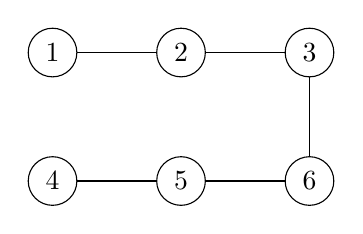
\begin{tikzpicture}[node distance=1cm, every node/.style={circle, draw, minimum size=0.30cm}]

    \node[fill=none] (1) {1};
    \node[fill=none, right =of 1] (2) {2};
    \node[fill=none,  right=of 2] (3) {3};
    \node[fill=none, below = of 1] (4) {4};
    \node[fill=none, below = of 2] (5) {5};
    \node[fill=none, below = of 3] (6) {6};
    \draw (1) -- (2);
    \draw (2) -- (3);
    \draw (4) -- (5);
    \draw (5) -- (6);
    \draw (6) -- (3);    
\end{tikzpicture}
\end{center}

$1-2-3-6-5-4-1$ is a Hamiltonian cycle

\begin{center}
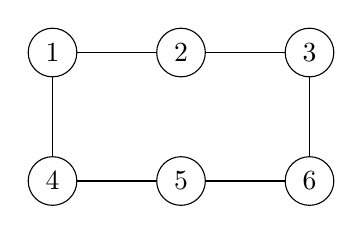
\begin{tikzpicture}[node distance=1cm, every node/.style={circle, draw, minimum size=0.30cm}]

    \node[fill=none] (1) {1};
    \node[fill=none, right =of 1] (2) {2};
    \node[fill=none,  right=of 2] (3) {3};
    \node[fill=none, below = of 1] (4) {4};
    \node[fill=none, below = of 2] (5) {5};
    \node[fill=none, below = of 3] (6) {6};
    \draw (1) -- (2);
    \draw (2) -- (3);
    \draw (4) -- (5);
    \draw (5) -- (6);
    \draw (6) -- (3);
    \draw (1) -- (4);
\end{tikzpicture}
\end{center}

\underline{Exercise}

Let $\mathcal{K}_n$ be a complete graph on $n-$vertices. How many cycles of size 3 does $\mathcal{K}_n$ contain? Size 4? Any size?

\underline{Fact}

Let $G_1$ be isomorphic to $G_2$. Then
\begin{enumerate}
    \item $g(G_1) = g(G_2) = girth(G_1) = girth(G_2)$
    \item $G_1$ has a Hamiltonian path/cycle if and only if $G_2$ does. 
\end{enumerate}

\subsection{Connectedness}

\underline{Definition}

Let $G$ be a graph. We say $G$ is connected if for all $v,u \in V(G)$, there exists a path from $v$ to $u$. 

\underline{Example}

\begin{center}
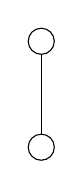
\begin{tikzpicture}[node distance=1cm, every node/.style={circle, draw, minimum size=0.30cm}]

    \node[fill=none] (1) {};
    \node[fill=none, below =of 1] (2) {};
   
    \draw (1) -- (2);    
\end{tikzpicture}
\end{center}

is the only 1-regular connected graph. 

2-regular connected graphs include

\begin{center}
\begin{tikzpicture}[node distance=1cm, every node/.style={circle, draw, minimum size=0.30cm}]
    \node[fill=none] (1) {};
    \node[fill=none, below=of 1] (2) {};
    \node[fill=none, right=of 1] (3) {};
    \node[below=of 3] (4) {};
    \draw (1) -- (2);
    \draw (1) -- (3);
    \draw (3) -- (4);
    \draw (2) -- (4);
    \begin{scope}[xshift=4cm, yshift=-1.5cm]
    \node[fill=none] (14) {};
    \node[above right=of 14] (15) {};
    \node [below right=of 15] (16) {};
    \draw (14) -- (15);
    \draw (14) -- (16);
    \draw (15) -- (16);
    \end{scope}
    \begin{scope}[xshift=10cm, every node/.style={circle, draw, minimum size=0.3cm}]

    \node[fill=none] (6) {};
    \node[below left=of 6] (7) {};
    \node [below=of 7] (8) {};
    \node [below right=of 8] (9) {};
    \node [right=of 9] (10) {};
    \node [above right=of 10] (11) {};
    \node [above=of 11] (12) {};
    \node [above left=of 12] (13) {};
    \draw (6) -- (7);
    \draw (7) -- (8);
    \draw (8) -- (9);
    \draw (9) -- (10);
    \draw (10) -- (11);
    \draw (11) -- (12);
    \draw (12) -- (13);
    \draw (13) -- (6);
    \end{scope}

\end{tikzpicture}
\end{center}


These are the only examples.

A complete graph is always a connected graph. 

\begin{center}
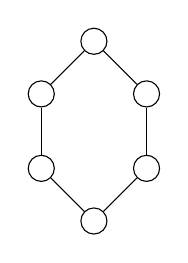
\begin{tikzpicture}[node distance=0.6cm, every node/.style={circle, draw, minimum size=0.30cm}]
    \node[fill=none] (1) {};
    \node[fill=none, below left =of 1] (2) {};
    \node[fill=none, below =of 2] (3) {};
    \node[fill=none, below right=of 3] (4) {};
    \node[fill=none, below right = of 1] (5) {};
    \node[fill = none, below=of 5] (6) {};
    \draw (1) -- (2);
    \draw (1) -- (5);
    \draw (3) -- (4);
    \draw (6) -- (4);
    \draw (2) -- (3);
    \draw (5) -- (6);
\end{tikzpicture}
\end{center}

This is true because there is always a path (of length 1) between two vertices. 

\underline{Theorem}

Let $G$ be a graph. Let $v \in V(G)$ be such that there is a walk from $v$ to $u$ for all $w \in V(G)$. Then $G$ is connected. 

\underline{Proof}

Let $u,w \in V(G)$. We know there exists a walk $u-u_2-u_3-\ldots-u_{n-1}-v$. There also exists a walk $w-w_2-w_3-\ldots-w_{m-1}-v$.

Hence there is a walk. 

$u-u_2-u_3-u_{n-1}-v-w_{m-1}-\ldots-w_2-w_1$

Hence there exists a path between $u$ and $w$ by previous result. Hence $G$ is connected. 

\underline{Theorem}

Let $G_1$ be isomorphic to $G_2$. Then $G_1$ is connected if and only if $G_2$ is connected. 

\underline{Definition}

Let $G$ be a graph. We say $G$ is disconnected if it is not connected. 

\underline{Example} 1-regular graph on 6 vertices

\begin{center}
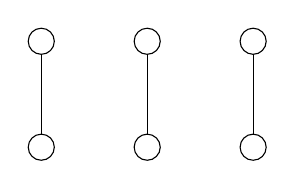
\begin{tikzpicture}[node distance=1cm, every node/.style={circle, draw, minimum size=0.30cm}]

    \node[fill=none] (1) {};
    \node[fill=none, below =of 1] (2) {};
    \node[fill=none, right =of 1] (3) {};
    \node[fill=none, below =of 3] (4) {};
    \node[fill=none, right =of 3] (5) {};
    \node[fill=none, below =of 5] (6) {};
   
    \draw (1) -- (2);
    \draw (3) -- (4);
    \draw (5) -- (6);
\end{tikzpicture}
\end{center}

Notice, both of the two graphs below are disconnected. But one is more disconnected than the other. 

\begin{center}
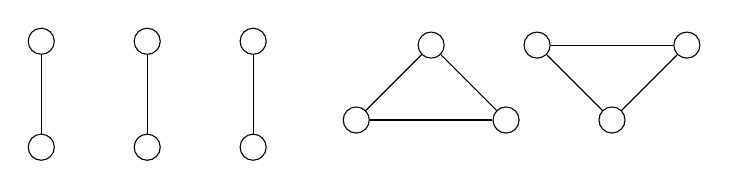
\begin{tikzpicture}[node distance=1cm, every node/.style={circle, draw, minimum size=0.30cm}]
    \node[fill=none] (1) {};
    \node[fill=none, below =of 1] (2) {};
    \node[fill=none, right =of 1] (3) {};
    \node[fill=none, below =of 3] (4) {};
    \node[fill=none, right =of 3] (5) {};
    \node[fill=none, below =of 5] (6) {};
    \draw (1) -- (2);
    \draw (3) -- (4);
    \draw (5) -- (6);
    \begin{scope}[xshift=4cm, yshift= -1cm]
    \node[fill=none] (6) {};
    \node[above right=of 6] (7) {};
    \node [below right=of 7] (8) {};
    \node [right=of 8] (11) {};
    \node [above left=of 11] (9) {};
    \node [above right=of 11] (10) {};
    \draw (6) -- (7);
    \draw (6) -- (8);
    \draw (7) -- (8);
    \draw (9) -- (10);
    \draw (9) -- (11);
    \draw (10) -- (11);
    \end{scope}
\end{tikzpicture}
\end{center}

\underline{Definition}

We say a subgraph $H$ is a component of $G$ if
\begin{enumerate}
    \item $H$ is connected
    \item $H$ is a subgraph of $G$ 
    \item If $H_2$ contains $H$ as a proper subgraph, then $H_2$ is disconnected.
\end{enumerate}

\underline{Example}

Consider
\begin{center}
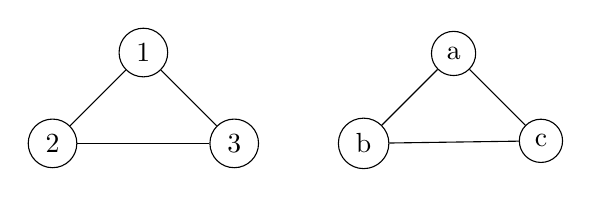
\begin{tikzpicture}[node distance=1cm, every node/.style={circle, draw, minimum size=0.30cm}]
    \node[fill=none] (1) {1};
    \node[fill=none, below left =of 1] (2) {2};
    \node[fill=none, below right =of 1] (3) {3};
    \node[fill=none, right =of 3] (4) {b};
    \node[fill=none, above right =of 4] (5) {a};
    \node[fill=none, below right =of 5] (6) {c};
    \draw (1) -- (2);
    \draw (1) -- (3);
    \draw (2) -- (3);
    \draw (5) -- (6);
    \draw (4) -- (6);
    \draw (4) -- (5);

\end{tikzpicture}

\begin{tikzpicture}[node distance=1cm, every node/.style={circle, draw, minimum size=0.30cm}]
    \node[fill=none] (1) {1};
    \node[fill=none, below left =of 1] (2) {2};

    \node[fill=none, right =of 3] (4) {b};
    \node[fill=none, above right =of 4] (5) {a};
    
    \draw (1) -- (2);
    \draw (4) -- (5);

\end{tikzpicture}
\end{center}

is not a component as it is not connected. 

\begin{center}
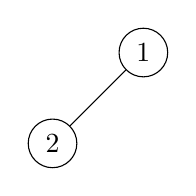
\begin{tikzpicture}[node distance=1cm, every node/.style={circle, draw, minimum size=0.30cm}]
    \node[fill=none] (1) {1};
    \node[fill=none, below left =of 1] (2) {2};
    \draw (1) -- (2);

\end{tikzpicture}
\end{center}

is not a component because it is a proper subgraph of the connected subgraph. 

\begin{center}
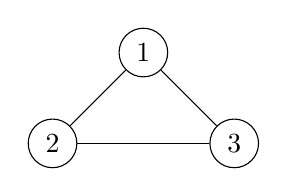
\begin{tikzpicture}[node distance=1cm, every node/.style={circle, draw, minimum size=0.30cm}]
    \node[fill=none] (1) {1};
    \node[fill=none, below left =of 1] (2) {2};
    \node[fill=none, below right =of 1] (3) {3};
    \draw (1) -- (2);
    \draw (1) -- (3);
    \draw (2) -- (3);

\end{tikzpicture}
\end{center}

In this case the two components are 

\begin{center}
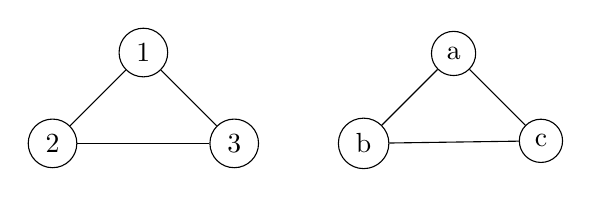
\begin{tikzpicture}[node distance=1cm, every node/.style={circle, draw, minimum size=0.30cm}]
    \node[fill=none] (1) {1};
    \node[fill=none, below left =of 1] (2) {2};
    \node[fill=none, below right =of 1] (3) {3};
    \node[fill=none, right =of 3] (4) {b};
    \node[fill=none, above right =of 4] (5) {a};
    \node[fill=none, below right =of 5] (6) {c};
    \draw (1) -- (2);
    \draw (1) -- (3);
    \draw (2) -- (3);
    \draw (5) -- (6);
    \draw (4) -- (6);
    \draw (4) -- (5);

\end{tikzpicture}
\end{center}

The number of components measures how disconnected a graph is.

\underline{Theorem}

Let $G_1$ be isomorphic to $G_2$. Then $G_1$ has the same number of components as $G_2$. 

\underline{Recall}

$H$ is a proper subgraph of $G$ if $H$ is a subgraph and either $V(H) \ne V(G)$ or $E(H) \ne E(G)$.


\underline{Definition}
Let $X \subseteq V(G)$. We define a cut induced by $X$ as the set of edges with one end in $X$ and one end outside of $X$. 

\underline{Example}

Let $X = \{1,2,3\}$ for the graph

\begin{center}
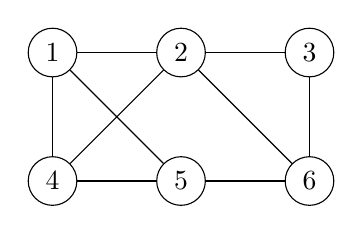
\begin{tikzpicture}[node distance=1cm, every node/.style={circle, draw, minimum size=0.30cm}]

    \node[fill=none] (1) {1};
    \node[fill=none, right =of 1] (2) {2};
    \node[fill=none,  right=of 2] (3) {3};
    \node[fill=none, below = of 1] (4) {4};
    \node[fill=none, below = of 2] (5) {5};
    \node[fill=none, below = of 3] (6) {6};
    \draw (2) -- (4);
    \draw (1) -- (4);
    \draw (1) -- (5);
    \draw (6) -- (3);
    \draw (2) -- (3);
    \draw (5) -- (6);
    \draw (2) -- (6);
    \draw (1) -- (2);
    \draw (4) -- (5);
    
\end{tikzpicture}
\end{center}

The edges in pink are those induced by the cut $X = \{1,2,3\}$

\begin{center}
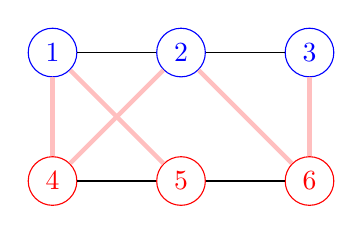
\begin{tikzpicture}[node distance=1cm, every node/.style={circle, draw, minimum size=0.30cm}]


    \node[color = blue,fill=none] (1) {1};
    \node[color = blue,fill=none, right =of 1] (2) {2};
    \node[color = blue,fill=none,  right=of 2] (3) {3};
    \node[color = red,fill=none, below = of 1] (4) {4};
    \node[color = red,fill=none, below = of 2] (5) {5};
    \node[color = red,fill=none, below = of 3] (6) {6};

    \draw (2) [pink, ultra thick] -- (4);
    \draw (1) [pink, ultra thick] -- (4);
    \draw (1) [pink, ultra thick]-- (5);
    \draw (6) [pink, ultra thick]-- (3);
    \draw (2) -- (3);
    \draw (5) -- (6);
    \draw (2) [pink, ultra thick]-- (6);
    \draw (1) -- (2);
    \draw (4) -- (5);
    
\end{tikzpicture}
\end{center}

\underline{Example}

Find a non-empty, proper set $X \subseteq V(G)$ such that the cut induced by $X$ is empty. 

\begin{center}
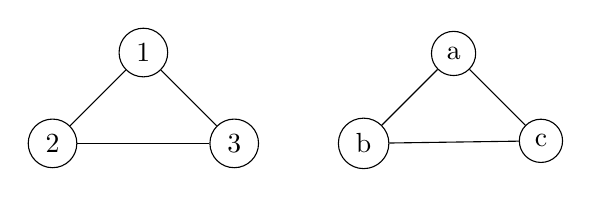
\begin{tikzpicture}[node distance=1cm, every node/.style={circle, draw, minimum size=0.30cm}]

    \node[fill=none] (1) {1};
    \node[fill=none, below left =of 1] (2) {2};
    \node[fill=none, below right =of 1] (3) {3};
    \node[fill=none, right =of 3] (4) {b};
    \node[fill=none, above right =of 4] (5) {a};
    \node[fill=none, below right =of 5] (6) {c};
    \draw (1) -- (2);
    \draw (1) -- (3);
    \draw (2) -- (3);
    \draw (5) -- (6);
    \draw (4) -- (6);
    \draw (4) -- (5);

\end{tikzpicture}
\end{center}

Notice the cut induced by $\{1,2,3\}$ is empty. We could have alternatively used $\{a,b,c\}$ to get a similar result. 

\underline{Example}

Can we find a proper non-empty set $X \subseteq V(G)$ such that the cut induced by $X$ is empty?

\begin{center}
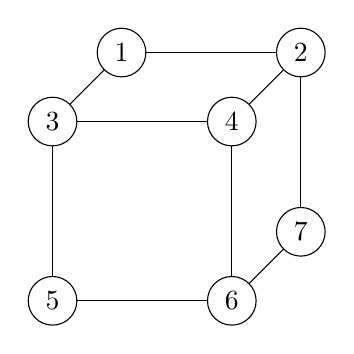
\begin{tikzpicture}[node distance=0.4cm, every node/.style={circle, draw, minimum size=0.30cm}, scale=0.08cm]

    
    \coordinate (B) at (1,0,0);
    \coordinate (C) at (1,1,0);
    \coordinate (D) at (0,1,0);
    \coordinate (E) at (0,0,1);
    \coordinate (F) at (1,0,1);
    \coordinate (G) at (1,1,1);
    \coordinate (H) at (0,1,1);
    
    \draw (D) -- (C) -- (B);
    \draw (E) -- (F) -- (G) -- (H) -- cycle;
    \draw (B) -- (F);
    \draw (C) -- (G);
    \draw (D) -- (H);
    
    \foreach \i/\name in {B/7, C/2, D/1, E/5, F/6, G/4, H/3} {
        \node at (\i) [circle, fill=white] {\name};
    }
  
\end{tikzpicture}
\end{center}

Assume $1 \in X$. (If $1 \not\in X$, a similar argument holds). As $(1,2) \in E(G)$, and we want the cut to be empty, we must have $2 \in X$. 

Similarly, $3 \in X$ as $(1,3) \in E(G)$. Similarly, $4,5,6$ and $7$ are all in $X$. Hence $X$ is not a proper subset of $V(G)$.

If we instead assumed $1 \not\in X$, we could show $2,3,4,5,6$ and $7$ are not in $X$, hence $X$ would be empty. 

\underline{Recall}

\underline{Definition}

Let $X \subseteq V(G)$. We say that the cut induced by $X$ is the set of edges $(v_1, v_2) \in E(G)$ such that $v_1 \in X$ and $v_2 \in V(G) \setminus X$. 

\underline{Theorem}

A graph is disconnected if and only if there exists a non-empty proper $X \subseteq V(G)$ such that the cut induced by $X$ is empty. 

Note: Proper means $X \subseteq V(G)$ and $X \ne V(G)$ (strict subset). 

\underline{Proof}

Assume $G_1$ is disconnected. 

Hence there exists $x,y \in V(G)$ such that there is no path between $x$ and $y$. 

Let $X$ by the set of vertices connected to $x$ by a path. We see $x \in X$, hence $X$ is non-empty. Further, $y \ne X$, hence it is proper. 

Consider $(v_1, v_2)$ in the cut induced by $X$. Assume $v_1 \in X$, $v_2 \not\in X$. Assume $v_1 \in X$, $v_2 \not\in X$. There is a path from $x$ to $v_1$ and from $v_1$ to $v_2$, hence from $x$ to $v_2$, a contradiction. The cut induced by $X$ is empty. 

Assume for the other direction there exists a non-empty proper $X$ such that the cut induced by $X$ is empty. 

There exists $x \in X$ and $y \not\in X$. We want to show there is no path between $x$ and $y$. Assume for contradiction that $x-v_1-v_2 - \ldots -v_n -y$ is such a path. 

Let $k$ be the maximal term such that $v_k \in X$, $v_{k+1} \not\in X$. (Let $x = v_0, y = v_{n+1}$). Then ($v_k, v_{k+1}$) is an edge in the cut induced by $X$, which is supposed to be empty. 

\subsection{Euler Tours}

\underline{Eulerian Circuits}

Example (Königsberg, $18^{\text{th}}$ century)

\begin{center}
\tikzset{sketch/.style={decorate,
 decoration={random steps, amplitude=1pt, segment length=5pt}, 
 line join=round, draw=black!80, very thick, fill=#1
}}
\begin{tikzpicture}

\clip [preaction={fill=cyan!10}] (0,0) rectangle (10,10);

\foreach \p/\r/\w/\h in 
  {(3,1)/5/1/4, (3,9)/-5/1/-4, (5,1)/-5/0.75/4, (5,9)/5/0.75/-4, 
  (5,5)/-90/0.75/4, (5,1)/-50/1/4, (6,8)/50/0.75/-4}
\draw [sketch=yellow!25]
   [shift={\p}, rotate=\r] rectangle +(\w,\h);

\draw [sketch=green!50]
  (-1,-1) -- (-1,0) to [bend left, looseness=0.5] (6,2) to [bend left] (7,-1) 
  (11,-1) to [bend left] (8,6) to [bend left] (11,6) -- cycle
  (-1,9) to [bend right, looseness=0.5] (7,8) to [bend left] 
  (11,9) -- (11,11) -- (-1,11) -- cycle
  (2,4) to [bend left, looseness=0.5] (2.5,6) to [bend left] 
  (6,6) to [bend left] (6,3.5) to [bend left] (2,4) -- cycle;
\end{tikzpicture}

The map above is actually not an image. It's TikZ. See source code \href{https://tex.stackexchange.com/questions/183882/drawing-k%C3%B6nigsberg-landscape-showing-the-bridges}{here}.
\end{center}

\underline{Question}

Can we take a walk from your house, crossing every bridge exactly once, and end up back at your house. 

We can translate this question to a graph, and walk on a graph. 

\begin{center}
\begin{tikzpicture}[node distance=1cm, every node/.style={circle, draw, minimum size=0.30cm}]
    \node[fill=none] (1) {A};
    \node[fill=none, below =of 1] (2) {B};
    \node[fill=none, below  =of 2] (3) {C};
    \node[fill=none, right =of 2] (4) {D};
    \draw (1) to[out=260, in=100, looseness=1] (2);
    \draw (1) to[out=280, in=80, looseness=1] (2);
    \draw (2) to[out=260, in=100, looseness=1] (3);
    \draw (2) to[out=280, in=80, looseness=1] (3);
    \draw (3) -- (4);
    \draw (4) -- (1);
    \draw (4) -- (2);
\end{tikzpicture}
\end{center}

\underline{Question (Revised)}

Does there exist a walk starting and ending at the same vertex that goes through every edge exactly once. 

This is not possible (for this graph). 

We see every time such a walk goes through a vertex, it must enter and exit via different edges. Hence if it is visited $k$ times, the vertex has degree $2k$.

That is, every vertex has even degree. 

In this case, $\deg(A) = \deg(C) = \deg(D) = 3$ and $\deg(B) = 5$. None of these have even degree. 

Hence such a walk does not exist for this graph. 

\underline{Definition}

An Eulerian Circuit is a walk that starts and ends at the same vertex and goes through every edge exactly once. 

\underline{Definition}

An Eulerian walk is a walk that goes through every edge exactly once. This means start and end at different locations. 

Example: Modern day Kaliningrad

\begin{center}
\tikzset{sketch/.style={decorate,
 decoration={random steps, amplitude=1pt, segment length=5pt}, 
 line join=round, draw=black!80, very thick, fill=#1
}}
\begin{tikzpicture}

\clip [preaction={fill=cyan!10}] (0,0) rectangle (10,10);

\foreach \p/\r/\w/\h in 
  {(4,1)/-5/0.75/4, (4,9)/5/0.75/-4, 
  (5,5)/-90/0.75/4, (5,1)/-50/1/4, (6,8)/50/0.75/-4}
\draw [sketch=yellow!25]
   [shift={\p}, rotate=\r] rectangle +(\w,\h);

\draw [sketch=green!50]
  (-1,-1) -- (-1,0) to [bend left, looseness=0.5] (6,2) to [bend left] (7,-1) 
  (11,-1) to [bend left] (8,6) to [bend left] (11,6) -- cycle
  (-1,9) to [bend right, looseness=0.5] (7,8) to [bend left] 
  (11,9) -- (11,11) -- (-1,11) -- cycle
  (2,4) to [bend left, looseness=0.5] (2.5,6) to [bend left] 
  (6,6) to [bend left] (6,3.5) to [bend left] (2,4) -- cycle;
\end{tikzpicture}

\begin{tikzpicture}[node distance=0.7cm, every node/.style={circle, draw, minimum size=0.30cm}]
    \node[fill=none] (1) {A};
    \node[fill=none, below =of 1] (2) {B};
    \node[fill=none, below  =of 2] (3) {C};
    \node[fill=none, right =of 2] (4) {D};
    \draw (1) --(2);
    \draw (2) -- (3);
    \draw (3) -- (4);
    \draw (4) -- (1);
    \draw (4) -- (2);
\end{tikzpicture}
\end{center}

$B-A-D-B-C-D$ is an Eulerian walk. 

\underline{Question}

Is it always possible to find an Eulerian circuit if all vertices have even degree

\underline{Answer}

If $G$ is disconnected, no. If $G$ is connected, then yes. We prove this by induction. 

\underline{Theorem}

Let $G$ be a connected graph such that every vertex has even degree. Then $G$ has an Eulerian Circuit. 

Note: This proof also works for multiedges and loops. 

\underline{Proof}

We will do this by induction on the number of edges in the graph

\underline{Cases}

\begin{center}
\begin{tikzpicture}[node distance=0.7cm, every node/.style={circle, draw, minimum size=0.30cm}]
    \node[fill=none] (1) {};
    \node[fill=none, right=of 1] (2) {};
    \node[fill=none, right=of 2] (3) {};
    \node[fill=none, right=of 3] (4) {};
    \node[fill=none, right=of 4] (5) {};
    \node[fill=none, above right=of 5] (6) {};
    \node[fill=none, below right=of 5] (7) {};

    \draw (2) to[out = 340, in = 20, loop, looseness=6] (2);
    \draw (3) to[out = 20, in = 160] (4);
    \draw (4) to[out = 200, in = 340] (3);
    \draw (5) -- (6);
    \draw (5) -- (7);
    \draw (6) -- (7);
\end{tikzpicture}
\end{center}

Assume the statement is true for every connected graph with ($m$ or fewer)$-$edges.

Notice, every vertex has degree at least 2. 

Hence $G$ will have a cycle
\begin{align*}
    v_1 - v_2 - \ldots - v_{n-1} - v_1
\end{align*}

We remove this cycle from the edge set of the graph. 

Every vertex will have even degree. Every component will have $m$ or fewer edges. Hence every component has an Eulerian circuit. Further, every component shares a vertex with the cycle. We now glue things together. 

I.e. component with circuit $v_i - w_1 - w_2 - \ldots -w_m - v_i$

We stick this in as $v_1 - v_2 - \ldots - v_3 - w_1 - \ldots - w_m - v_i -v_{i+1}$

\underline{Eulerian Circuits}

\underline{Recall}

An Eulerian circuit is a walk starting and ending at the same vertex and using every edge exactly once. 

We showed that if $G$ was connected and all vertices had an even degree, then $G$ had an Eulerian circuit

\underline{Example}

\begin{center}
\begin{tikzpicture}[node distance=1cm, every node/.style={circle, draw, minimum size=0.30cm}]
    \node[fill=none] (1) {1};
    \node[fill=none, right =of 1] (2) {2};
    \node[fill=none,  right=of 2] (3) {3};
    \node[fill=none, below = of 1] (4) {4};
    \node[fill=none, below = of 2] (5) {5};
    \node[fill=none, below = of 3] (6) {6};
    \draw (1) -- (4);
    \draw (2) -- (6);
    \draw (6) to[out=200, in = 350, looseness=1] (5);
    \draw (1) -- (2);
    \draw (2) -- (5);
    \draw (2) -- (3);
    \draw (6) -- (3);
    \draw (5) -- (6);
    \draw (4) to[out = 270, in = 180, looseness=5] (4);
    \draw (4) -- (5);
\end{tikzpicture}
\end{center}

\underline{Step 1}

Find a cycle. 

For example $1-2-3-6-5-4-1$

\underline{Step 2}

Remove this cycle from the graph to get a number of components. 

\begin{center}
\begin{tikzpicture}[node distance=1cm, every node/.style={circle, draw, minimum size=0.30cm}]
    \node[fill=none] (1) {1};
    \node[fill=none, right =of 1] (2) {2};
    \node[fill=none,  right=of 2] (3) {3};
    \node[fill=none, below = of 1] (4) {4};
    \node[fill=none, below = of 2] (5) {5};
    \node[fill=none, below = of 3] (6) {6};
    \draw (2) -- (6);
    \draw (2) -- (5);
    \draw (6) -- (3);
    \draw (5) -- (6);
    \draw (4) to[out = 270, in = 180, looseness=5] (4);
\end{tikzpicture}
\end{center}

Repeat arguments on components to get the two cycles. 
\begin{align*}
    &1-2-3-6-5-4-1 \\
    &1-2-6-5-2-3-6-5-4-4-1
\end{align*}

\underline{Note}

A similar proof works for Eulerian Paths. A 45 bridge version exists in Bristol. 


\subsection{Bridges / Cut-edges}

\underline{Definition}

An edge is a bridge (or cut edge) if removing this edge produces a graph with moire components. 

Example

\begin{center}
\begin{tikzpicture}[node distance=1cm, every node/.style={circle, draw, minimum size=0.30cm}]
    \node[fill=none] (1) {1};
    \node[fill=none, right =of 1] (2) {2};
    \node[fill=none,  right=of 2] (3) {3};
    \node[fill=none, right = of 3] (4) {4};
    \node[fill=none, below = of 1] (5) {5};
    \node[fill=none, right = of 5] (6) {6};
    \node[fill=none, right = of 6] (7) {7};
    \node[fill=none, right = of 7] (8) {8};
    \draw (1) -- (2);
    \draw (1) -- (5);
    \draw (5) -- (2);
    \draw (2) -- (6);
    \draw (6) -- (7);
    \draw (6) -- (3);
    \draw (3) -- (7);
    \draw (3) -- (8);
    \draw (8) -- (4);
    \draw (7) -- (8);
    
\end{tikzpicture}
\end{center}

The edge (2,6) is a bridge. After removing this edge we get two components. 

The edge (4,8) is also a bridge. 

\underline{Theorem}

If $e$ is a bridge of a connected graph $G$, then $G \setminus \{e\}$ has two components. 

The two components will be the set of vertices in $G \setminus \{(v,w)\}$ connected to $v$, say $V$. Similarly for $u$, say $U$. 

(Here "connected to" means there exists a path from $u$ to this vertex). 

If $x \in V$ then there is no path from $v$ to $x$ in $G \setminus \{e\}$. 

There is a path from $v$ to $x$ in $G$. 

This means the path goes through the edge $(v,x)$. Hence there is a path from $u$ to $x$. 

Hence for any vertex $x$, if $x \not\in V$, then $x \in U$, and if $x \not\in U$, then $x \in V$. 

Hence $G \setminus \{(v,u)\}$ has two components. 

\underline{Example}
\begin{center}
\begin{tikzpicture}[node distance=1cm, every node/.style={circle, draw, minimum size=0.30cm}]
    \node[fill=none] (1) {1};
    \node[fill=none, right =of 1] (2) {2};
    \node[fill=none,  right=of 2] (3) {3};
    \node[fill=none, right = of 3] (4) {4};
    \node[fill=none, below = of 1] (5) {5};
    \node[fill=none, right = of 5] (6) {6};
    \node[fill=none, right = of 6] (7) {7};
    \node[fill=none, right = of 7] (8) {8};
    \draw (1) -- (2);
    \draw (1) -- (5);
    \draw (5) -- (2);
    \draw (2) -- (6);
    \draw (6) -- (7);
    \draw (6) -- (3);
    \draw (3) -- (7);
    \draw (3) -- (8);
    \draw (8) -- (4);
    \draw (7) -- (8);
    
\end{tikzpicture}
\end{center}

Notice that an edge in the previous graph is either contained in a cycle, or a bridge, but not both. 

\underline{Theorem}

An edge is a bridge if and only if it is not in a cycle. 

\underline{Equivalently}

\underline{Theorem}

An edge is not a bridge if and only if it is not contained in a cycle. 

\underline{Proof}

Let $(v,w)$ be in a cycle, say
\begin{align*}
    v-u-u_2-u_3-\ldots-u_n-v
\end{align*}
removing $(v,u)$ leaves a graph where $v$ has a path to $u$. 

This gives, the set of vertices with a path to $v$ is the same set as the set of vertices with a path to $u$. Hence we have the same number of components. 

Assume next that $(u,v)$ is not a bridge. If we remove this edge, we still have a path from $u$ to $v$, say
\begin{align*}
    u_1-u_2-\ldots-u_n-v
\end{align*}
This gives that
\begin{align*}
    u-u_2-u_3-\ldots-u_n-v-u
\end{align*}
is a cycle in $G$.

\underline{Theorem}

If there exists two distinct paths from $u$ to $v$, then the graph contains a cycle. 

\underline{Example}

\begin{center}
\begin{tikzpicture}[node distance=1cm, every node/.style={circle, draw, minimum size=0.30cm}]
    \node[fill=none] (1) {1};
    \node[fill=none, right =of 1] (2) {2};
    \node[fill=none, above right = of 2] (3) {3};
    \node[fill=none, below right = of 2] (4) {4};
    \node[fill=none, below right = of 3] (5) {5};
    \node[fill=none, right=of 5] (6) {6};
    \draw (1) -- (2);
    \draw (2) -- (3);
    \draw (2) -- (4);
    \draw (4) -- (5);
    \draw (3) -- (5);
    \draw (5) -- (6);
    
\end{tikzpicture}
\end{center}

This has two distinct paths from 1 to 6. Namely, 
\begin{align*}
    1-2-3-5-6\\
    1-2-4-5-6
\end{align*}

Notice if we remove the edge $(2,3)$ that there exists a walk from 2 to 3. We go
\begin{align*}
    2-1-2-4-5-6-5-3
\end{align*}

Hence there exists a path from 2 to 3 without the edge $(2,3)$. This is $2-4-5-3$. 

Adding the edge back in gives a cycle $2-4-5-3-2$

How could we prove this in general?

\underline{Theorem}

If there exists two different paths from $u$ to $v$, then $G$ has a cycle. 

\underline{Proof}

Take an edge that is in one path but not in the other. 

If we remove this edge, then we still have the same number of components. Hence this edge is not a bridge. Hence this graph has a cycle. 

\section{Trees}

\subsection{Trees and Minimally Connected Graphs}

\underline{Definition}

A graph is a tree if it contains no cycle and it is connected. 

\underline{Example}

\begin{center}
\begin{tikzpicture}[node distance=1cm, every node/.style={circle, draw, minimum size=0.30cm}]

    \definecolor{mydarkgreen}{RGB}{0,100,0}

    \node[fill=mydarkgreen] (1) {};
    \node[fill=none, right =of 1] (2) {};
    \node[fill=mydarkgreen, above =of 2] (3) {};
    \node[fill=mydarkgreen, below left =of 2] (4) {};
    \node[fill=mydarkgreen, below right =of 2] (5) {};
    \node[fill=mydarkgreen, above right =of 2] (6) {};
    \node[fill=none, below right =of 6] (7) {};
    \node[fill=mydarkgreen, right =of 7] (8) {};
    \node[fill=mydarkgreen, below =of 7] (9) {};
   
    \draw (1) -- (2);
    \draw (2) -- (3);
    \draw (2) -- (4);
    \draw (2) -- (5);
    \draw (2) -- (6);
    \draw (2) -- (7);
    \draw (7) -- (8);
    \draw (7) -- (9);
\end{tikzpicture}
\end{center}


\underline{Definition}

We call this graph a forest if every component is a tree. 

\underline{Definition}

Let $T$ be a tree. A vertex $v \in V(T)$ is a leaf if it has degree 1. 

\underline{Example}

A $1-$regular graph is a forest, and every vertex is a leaf. 
\begin{center}
\begin{tikzpicture}[node distance=1cm, every node/.style={circle, draw, minimum size=0.30cm}]
    \definecolor{mydarkgreen}{RGB}{0,100,0}

    \node[fill=mydarkgreen] (1) {};
    \node[fill=mydarkgreen, below =of 1] (2) {};
    \node[fill=mydarkgreen, right =of 1] (3) {};
    \node[fill=mydarkgreen, below =of 3] (4) {};
    \node[fill=mydarkgreen, right =of 3] (5) {};
    \node[fill=mydarkgreen, below =of 5] (6) {};
   
    \draw (1) -- (2);
    \draw (3) -- (4);
    \draw (5) -- (6);
\end{tikzpicture}
\end{center}

\underline{Theorem}

Let $T$ be a tree. Then there is a unique path from $u$ to $v$ for all $u,v \in V(T)$. 

\underline{Proof}

Our tree is connected, hence there is a path. If there existed two distinct paths, then $T$ would have a cycle. Trees have no cycles. Hence the path is unique. 
\begin{center}
\begin{tikzpicture}[node distance=1cm, every node/.style={circle, draw, minimum size=0.40cm}]
    \node[fill=none] (1) {};
    \node[fill=none, below =of 1] (2) {};
    \node[fill=none, right =of 1] (3) {};
    \node[fill=none, right =of 3] (4) {};
    \node[fill=none, below right =of 4] (5) {};
    \node[fill=none, above right =of 5] (6) {};
    \node[fill=none, below right =of 5] (7) {}; 
   
    \draw (1) -- (3);
    \draw (2) -- (3);
    \draw (3) -- (4);
    \draw (4) -- (5);
    \draw (5) -- (6);
    \draw (5) -- (7);
    
\end{tikzpicture}
\end{center}

\underline{Theorem}

Let $T$ be a tree. Then every edge is a bridge. 

\underline{Proof}

If we had an edge that was not a bridge, then it is in a cycle. Trees have no cycles. Hence every edge is a bridge. 

\underline{Note} This is also true for forests. 

Question: What is the relationship between $|V(T)|$ and $|E(T)|$

Example ($G_1, G_2, G_3$ respectively). 
\begin{center}
\begin{tikzpicture}[node distance=1cm, every node/.style={circle, draw, minimum size=0.15cm}]

  \node (1) {};
  \node[below right=of 1] (2) {};
  \node[below left=of 2] (3) {};
  \node[above right=of 2] (4) {};
  \node[below right=of 2] (5) {};

  \foreach \i/\j in {1/2, 2/3, 2/4, 2/5} {
    \draw (\i) -- (\j);
  }


  \begin{scope}[xshift=4cm, yshift=-1.5cm]
  \node (6) {};
  \node[below right=of 6] (7) {};
  \node[above right=of 7] (8) {};
  \node[above =of 8] (9) {};
  
  \foreach \i/\j in {6/7, 7/8, 8/9} {
    \draw (\i) -- (\j);
  }
    
    \end{scope}

    \begin{scope}[xshift=8cm,yshift=-1cm]
    
    \node (10) {};
    \node [right =of 10] (11) {};
    \node [right= of 11] (12) {};
    \node [below=of 12] (13) {};
    \node [left =of 13] (14) {};
    \node [left =of 14] (15) {};
    \node [above = of 11] (16) {};
    
    \foreach \i/\j in {10/11, 11/16, 11/12, 12/13, 13/14, 15/14} {
    \draw (\i) -- (\j);
  }
    
    \end{scope}
\end{tikzpicture}
\end{center}

\begin{table}[h]
    \begin{tabular}{c|c|c|c} 
         & $G_1$ & $G_2$ & $G_3$\\ \hline 
         $|V(T)|$& $5$ & $4$ & $7$\\ 
         $|E(T)|$& $4$ & $3$ & $6$\\ 
    \end{tabular}
\end{table}



\underline{Theorem}

Let $T$ be a tree. Then $|E(T)| = |V(T)| - 1$

\underline{Proof}

We will use induction on the number of vertices. 

\underline{Base Case}

$1-$vertex $\implies 0$ edges

$2-$vertices $\implies 1$ edge

\underline{Inductive Hypothesis}

Assume this is true for all trees with $m$ or fewer vertices. 

\underline{Inductive Step}

Let $T$ be a tree with $m+1$ vertices. As $T$ is connected, there is a path from every $u$ to $v$, and hence there is an edge. This edge is a bridge. 

If we remove this bridge, we have two components, each a tree, and each with $m$ or fewer vertices. 

Let the first component be a tree with $s$ vertices, and the seconds have $t$ vertices. We have $s,t \le m$ and $s + t = m + 1$

By induction, the first tree has $s-1$ edges. The second has $t-1$ edges. This gives us that the original tree with $m+1$ vertices has 
\begin{align*}
    \underbrace{(s-1)}_{\text{first tree}} + \underbrace{(t-1)}_{\text{second tree}} + \underbrace{1}_{\text{bridge}} = s + t - 1 = m
\end{align*}

\underline{Example}
\begin{center}
\begin{tikzpicture}[node distance=1cm, every node/.style={circle, draw, minimum size=0.30cm}]

    \node[fill=none] (1) {};
    \node[fill=none, below right =of 1] (2) {};
    \node[fill=none, above right =of 2] (3) {};
    \node[fill=none, below  =of 2] (4) {};
    \node[fill=none, above right =of 4] (5) {};
    \node[fill=none, above right =of 5] (6) {};
    \node[fill=none, below =of 6] (7) {};
    \node[fill=none, right =of 6] (8) {};
    \node[fill=none, above right =of 8] (9) {};
    \node[fill=none, below right =of 8] (10) {};

   \draw (1) -- (2);
   \draw (2) -- (3);
   \draw (2) -- (4);
   \draw (4) -- (5);
   \draw (5) -- (6) [dashed];
   \draw (6) -- (7);
   \draw (6) -- (8);
   \draw (8) -- (9);
   \draw (8) -- (10);
\end{tikzpicture}
\end{center}

This gives 10 vertices in total and $4 + 4 + 1 = 9$ edges. 

How many leaves does a tree have?

\begin{center}
\begin{tikzpicture}[node distance=1cm, every node/.style={circle, draw, minimum size=0.15cm}]

  \node (1) {};
  \node[below right=of 1] (2) {};
  \node[below left=of 2] (3) {};
  \node[above right=of 2] (4) {};
  \node[below right=of 2] (5) {};

  \foreach \i/\j in {1/2, 2/3, 2/4, 2/5} {
    \draw (\i) -- (\j);
  }
  \node[draw=none, above=0.7cm] at (1) {$4$};


  \begin{scope}[xshift=4cm, yshift=-0.5cm]
  \node (6) {};
  \node[below right=of 6] (7) {};
  \node[above right=of 7] (8) {};
  \node[above right =of 8] (9) {};
  \node[below right=of 8] (10) {};
  
  \foreach \i/\j in {6/7, 7/8, 8/9, 8/10} {
    \draw (\i) -- (\j);
  }
  \node[draw=none, above =1.2cm] at (6) {$3$};
    
    \end{scope}

    \begin{scope}[xshift=8cm, yshift=-0.5cm]
    
    \node (11) {};
    \node [below right =of 11] (12) {};
    \node [above right= of 12] (13) {};
    \node [below right=of 13] (14) {};
    \node [above right =of 14] (15) {};
    
    \foreach \i/\j in {11/12, 12/13, 13/14, 14/15} {
    \draw (\i) -- (\j);
  }
  \node[draw=none, above=1.2cm] at (11) {$2$};
    
    \end{scope}
\end{tikzpicture}
\end{center}

\underline{Question}

Can a tree with $p$ vertices have fewer than 2 leaves, or more than $p-1$ leaves?

\underline{Theorem}

Let $T$ be a tree. Then $t$ has at least 2 leaves. (We assume $|V(T)| \ge 2$). 

\underline{Proof}

By induction

\underline{Base Case}

$2-$vertices $\implies 2$ leaves

Both vertices are leaves. $T$ has 2 leaves. 

\underline{Inductive Hypothesis}

Assume this is true for every tree with $m$ or fewer vertices. 

\underline{Inductive Step}

Let $T$ be a tree with $m+1$ vertices. This tree will have an edge and this edge is a bridge. 

Call this edge $(u,v)$. Let the two trees that result from removing this bridge be $U$ and $V$. 

\begin{center}
\begin{tikzpicture}[node distance=1cm, every node/.style={circle, draw, minimum size=0.30cm}]

    \node[fill=none] (1) {};
    \node[fill=none, above left =of 1] (2) {};
    \node[fill=none, below left =of 1] (3) {};
    \node[fill=none, right=of 1] (4) {};
    \node[fill=none, above right =of 4] (5) {};
    \node[fill=none, below right =of 4] (6) {};
   
    \draw (1) -- (2);
    \draw (1) -- (3);
    \draw (1) -- (4);
    \draw (4) -- (5);
    \draw (4) -- (6);
\end{tikzpicture}
\end{center}

We have two cases. 

We could have $u$ is a leaf, and $v$ is not (or equivalently, $v$ is a leaf, $u$ is not) or both vertices are not leaves of $T$. 

\underline{Case 1:}

$u$ is a leaf of $T$, $v$ is not. Hence by induction $V$ will have two leaves. It is possible one of these is $v$. One of these is not $v$, call it $w$. 

We can check that $u$ and $w$ are leaves of $T$. 

\begin{center}
\begin{tikzpicture}[node distance=1cm, every node/.style={circle, draw, minimum size=0.30cm}]

    \node[fill=none] (1) {$u$};
    \node[fill=none, right=of 1] (2) {$v$};
    \node[fill=none, right=of 2] (3) {};
    \node[fill=none, right=of 3] (4) {};
    \node[fill=none, right =of 4] (5) {$w$};
   
    \draw (1) -- (2);
    \draw (2) -- (3);
    \draw (3) -- (4);
    \draw (4) -- (5);
\end{tikzpicture}
\end{center}

\underline{Case 2}

Neither $u$ and $v$ are leaves. 

As before, $U$ and $V$ will have two leaves. At least on of the leaves of $U$ is not $u$, call this $x$.

At least one of the leaves of $U$ is not $v$, call this $w$. Then $x$ and $w$ are leaves of $T$. 

\begin{center}
\begin{tikzpicture}[node distance=1cm, every node/.style={circle, draw, minimum size=0.50cm}]

    \node[fill=none] (1) {$w$};
    \node[fill=none, above left =of 1] (2) {$v$};
    \node[fill=none, below left =of 1] (3) {$u$};
    \node[fill=none, right=of 1] (4) {};
    \node[fill=none, above right =of 4] (5) {};
    \node[fill=none, below right =of 4] (6) {$x$};
   
    \draw (1) -- (2);
    \draw (1) -- (3);
    \draw (1) -- (4);
    \draw (4) -- (5);
    \draw (4) -- (6);
\end{tikzpicture}
\end{center}

\subsection{Spanning Trees}

\underline{Recall}

\underline{Definition}

We say a subgraph $H$ of $G$ is a spanning subgraph if $V(H) - V(G)$.

\underline{Definition}

We say $G$ is a tree if it contains no cycles and is connected. 

\underline{Definition}

We say $T$ is a spanning tree of $G$ if $T$ is a spanning subgraph of $G$ and it is a tree. 

\underline{Example}

Find a spanning tree of

\begin{center}
\begin{tikzpicture}[node distance=1cm, every node/.style={circle, draw, minimum size=0.30cm}]

    \node[fill=none] (1) {A};
    \node[fill=none, below right =of 1] (2) {C};
    \node[fill=none, above right =of 1] (3) {B};
    \node[fill=none, above right  =of 2] (4) {D};
    \node[fill=none, above right  =of 4] (5) {E};
    \node[fill=none, below right  =of 4] (6) {F};
    \node[fill=none, above right  =of 6] (7) {G};
    
   
   \draw[yellow,line width = 2pt,yshift=-0.7pt](3)--(5);
   \draw[yellow,line width = 2pt,yshift=-0.7pt](1)--(3);
   \draw[yellow,line width = 2pt,yshift=-0.7pt](3)--(2);
   \draw[yellow,line width = 2pt,yshift=-0.7pt](3)--(4);
   \draw[yellow,line width = 2pt,yshift=-0.7pt](7)--(5);
   \draw[yellow,line width = 2pt,yshift=-0.7pt](6)--(5);
   \draw (3) -- (5);
   \draw (1) -- (2);
   \draw (1) -- (3);
   \draw (2) -- (3);
   \draw (2) -- (4);
   \draw (3) -- (4);
   \draw (4) -- (5); 
   \draw (5) -- (6);
   \draw (6) -- (4);
   \draw (5) -- (7);
   \draw (4) -- (7);
   
\end{tikzpicture}
\end{center}

\underline{Example}

Does a $1-$regular graph on 4 vertices have a spanning tree?

\begin{center}
\begin{tikzpicture}[node distance=1cm, every node/.style={circle, draw, minimum size=0.30cm}]
    \node[fill=none] (1) {};
    \node[fill=none, below =of 1] (2) {};
    \node[fill=none, right =of 1] (3) {};
    \node[fill=none, below =of 3] (4) {};
    
    \draw (1) -- (2);
    \draw (3) -- (4);
\end{tikzpicture}
\end{center}

\underline{No} We cannot find an edge from the left two vertices to the right two vertices. There are no spanning subgraphs, hence no spanning trees. 


\underline{Theorem}

A graph $G$ has a spanning tree if and only if $G$ is connected. 

\underline{Proof}

Assume first that $G$ has a spanning tree, say $T$. 

Take any two vertices in $G$, say $u$ and $v$. Then $u,v \in V(T)$ as $T$ is a spanning subgraph. 

As $T$ is a tree, there exists a (unique) path from $u$ to $v$. This path uses edges in $E(G)$. Hence there exists a path from $u$ to $v$ in $G$. This proves $G$ is connected. 

Assume for the other direction that $G$ is connected. 

$E(G)$ will contain some edges that are bridges, and some that are not. We will construct our spanning tree by removing non-bridge edges. 

Create a subgraph of $G$ by removing an edge that is not a bridge. If no such edge exists, we have a tree. Repeat this process on this new subgraph as needed. 

\begin{enumerate}
    \item We never remove a vertex, so all of these subgraphs are spanning. 
    \item We never remove a bridge, hence all of these subgraphs are connected. 
    \item At some point this process will step (I.e. when $|E(H)| = |V(H)| -1$)
\end{enumerate}

The result after repeating this will be a spanning connected subgraph where every edge is a bridge. I.e., a spanning tree. 

\underline{Example}

Find a spanning tree of the $4 \times 4$ graph

\begin{center}
\begin{tikzpicture}[node distance=1cm, every node/.style={circle, draw, minimum size=0.30cm}]
    \foreach \i in {0,...,3} {
        \foreach \j in {0,...,3} {
            \node[fill=none] (\i-\j) at (\i,\j) {};
        }
    }
    \draw (0-0) --  (0-1) -- (0-2) -- (0-3) -- (1-3) -- (2-3) -- (3-3) -- (3-2) -- (3-1) -- (3-0) -- (2-0) -- (1-0) -- (0-0);
    \draw (0-0) [red] -- (1-0);
    \draw (0-3) [red] -- (1-3) -- (2-3);
    \draw (3-1) [red] -- (3-2);
    \draw (1-1) [red]-- (1-2);
    \draw (1-2) -- (2-2);
    \draw (2-2) -- (2-1);
    \draw (2-1) [red]-- (1-1);
    \draw (0-1) -- (1-1);
    \draw (0-2) -- (1-2);
    \draw (1-2) -- (1-3);
    \draw (1-0) -- (1-1);
    \draw (2-3) -- (2-2);
    \draw (2-2) [red]-- (3-2);
    \draw (2-0) [red]-- (2-1);
    \draw (2-1) [red]-- (3-1);


    \begin{scope}[xshift=6cm]
    \foreach \i in {0,...,3} {
        \foreach \j in {0,...,3} {
            \node[fill=none] (\i-\j) at (\i,\j) {};
        }
    }
    \draw (0-0) -- (0-1) -- (0-2) -- (0-3);
    \draw (1-0) -- (2-0) -- (3-0) -- (3-1);
    \draw (2-3) -- (3-3) -- (3-2);
    \draw (1-2) -- (2-2);
    \draw (2-2) -- (2-1);
    \draw (0-1) -- (1-1);
    \draw (0-2) -- (1-2);
    \draw (1-2) -- (1-3);
    \draw (1-0) -- (1-1);
    \draw (2-3) -- (2-2);
    
    \end{scope}
    
\end{tikzpicture}
\end{center}

\underline{Method 2} - Grow the tree

Start with any vertex. This will be our starting (non-spanning) tree. 

Find any edge from inside this tree to outside this tree. Add this edge to get a larger tree. Repeat as necessary until you have every vertex. 

\underline{Example} Same as before

\begin{center}
\begin{tikzpicture}[node distance=1cm, every node/.style={circle, draw, minimum size=0.30cm}]
    \definecolor{mydarkgreen}{RGB}{0,100,0}
    \foreach \i in {0,...,3} {
        \foreach \j in {0,...,3} {
            \node[fill=none] (\i-\j) at (\i,\j) {};
        }
    }
    \node[fill=mydarkgreen] (0-0) {};
    \draw (0-0) -- node[draw=none, left] {1} (0-1);
    \draw (0-1) -- node[draw=none, above] {2} (1-1);
    \draw (2-1) -- node[draw=none, above] {12} (3-1);
    \draw (3-1) -- node[draw=none, right] {15} (3-0);
    \draw (1-1) -- node[draw=none, above] {9} (2-1);
    \draw (2-1) -- node[draw=none, right] {10} (2-0);
    \draw (2-0) -- node[draw=none, above] {11} (1-0);
    \draw (0-1) -- node[draw=none, left] {3} (0-2);
    \draw (0-2) -- node[draw=none, above] {4} (1-2);
    \draw (1-2) -- node[draw=none, right] {5} (1-3);
    \draw (1-2) -- node[draw=none, below] {8} (2-2);
    \draw (1-3) -- node[draw=none, above] {6} (0-3);
    \draw (1-3) -- node[draw=none, above] {7} (2-3);
    \draw (2-3) -- node[draw=none, above] {13} (3-3);
    \draw (3-3) -- node[draw=none, right] {14} (3-2);
    
\end{tikzpicture}
\end{center}

\subsection{Characterizing Bipartite Graphs}

Recall a graph $G$ is bipartite if there exists $A,B \subseteq V(G)$ where 
\begin{enumerate}
    \item $V(G) = A \cup B$
    \item $A \cap B = \emptyset$
    \item Every edge ($u,v$) has one end in $A$ and one end in $B$. 
\end{enumerate}

\underline{Theorem}

A cycle of odd length is not bipartite. 

\begin{center}
\begin{tikzpicture}[node distance=1cm, every node/.style={circle, draw, minimum size=0.30cm}, scale=0.03cm]

    \node[fill=none] (1) {};
    \node[fill=none, below left =of 1] (2) {};
    \node[fill=none, below right =of 1] (3) {};
    \draw (1) -- (2);
    \draw (1) -- (3);
    \draw (2) -- (3);

 \begin{scope}[xshift=4.5cm, yshift=-1cm]
    \def\radius{1.5cm}
    
    \foreach \i in {1,...,5} {
        \coordinate (P\i) at ({360/5 * (\i - 1)}:\radius);
    }
    
    \draw (P1) -- (P2) -- (P3) -- (P4) -- (P5) -- cycle;
    
    \foreach \i in {1,...,5} {
        \node at (P\i) [circle, draw, fill=white] {};
    }
    
    \end{scope}
\end{tikzpicture}
\end{center}

\underline{Proof}

Assume the graph is bipartite. 

Let $v$ be a vertex. Assume without loss of generality that $v \in A$. 

\begin{center}
\begin{tikzpicture}[node distance=1cm, every node/.style={circle, draw, minimum size=0.30cm}]

    \node[fill=none] (1) {1};
    \node[draw=none, fill=none, above right =of 1] (2) {A};
    \node[fill=none, below left =of 1] (3) {2};
    \node[draw=none, fill=none, above left=of 3] (4) {B};
    \node[fill=none, below=of 3] (5) {3};
    \node[draw=none, fill=none, above left=of 5] (6) {A};

    \node[fill=none, below right=of 1] (7) {4};
    \node[draw=none, fill=none, above right=of 7] (8) {B};
    \node[fill=none, below=of 7] (9) {5};
    \node[draw=none, fill=none, above right=of 9] (10) {A};
    
    \draw (1) -- (3);
    \draw [->] (2) -- (1);
    \draw (3) -- (5);
    \draw (1) -- (7);
    \draw (7) -- (9);
    \draw [->] (4) -- (3);
    \draw [->] (6) -- (5);
    \draw [->] (10) -- (9);
    \draw [->] (8) -- (7);
    
\end{tikzpicture}
\end{center}
The two adjacent vertices to $v$ are in $B$. 

The vertices adjacent to the vertices adjacent to $v$ are in $A$. (I.e. the vertices with a path of length 2 from $v$). 

Continue this process. Vertices with a path of length $1,3,5,\ldots$ are in $B$ and length $0,2,4,6,\ldots$ are in $A$. 

This is where the problem occurs, as there is a path of odd length from $v$ to $v$, hence it is in both $B$ and $A$. 

Hence the cycle is not bipartite. 

\underline{Corollary}

If $G$ contains a cycle of odd length, then it is not bipartite. 

\underline{Example}

\begin{center}
\begin{tikzpicture}[node distance=1cm, every node/.style={circle, draw, minimum size=0.30cm}]

    \node[fill=none] (1) {};
    \node[fill=none, below=of 1] (2){};
    \node[fill=none, below=of 2] (3){};
    \node[fill=none, right=of 3] (4){};
    \node[fill=none, above=of 4] (5){};
    \node[fill=none, above=of 5] (6) {};

    \node[fill=none, draw=none, below right=of 4] (7) {Bipartite};
    \node[fill=none, above right=of 7] (8) {};
    \node[fill=none, above=of 8] (9){};
    \node[fill=none, above=of 9] (10){};
    \node[fill=none, right=of 10] (11){};
    \node[fill=none, below=of 11] (12){};
    \node[fill=none, below=of 12] (13) {};

    

    \draw[->] (7) -- ($(7)!1.5cm!(4)$);
    \draw[->] (7) -- ($(7)!1.5cm!(8)$);
    \draw (1) -- (2) -- (3) -- (4) -- (5) -- (6) -- (1);
    \draw (2) -- (5);

    \draw (8) -- (9) -- (10) -- (11) -- (12) -- (13) -- (8);
    \draw (9) -- (12);
    \draw (10) -- (13);

    \begin{scope}[xshift=10cm, yshift=-4.05cm]
    \node[fill=none, draw=none] (14) {$\neg$ Bipartite};
    \node[fill=none, above left =of 14] (15) {};
    \node[fill=none, above right=of 14] (20) {};
    \node[fill=none, above=of 15] (16) {};
    \node[fill=none, above=of 16] (17) {};
    \node[fill=none, above=of 20] (18) {};
    \node[fill=none, above=of 18] (19) {};

    \draw (15) -- (16) -- (17) -- (18) -- (16);
    \draw (20) -- (18) -- (19) -- (17);
    \draw (20) -- (15);
    
    \end{scope}


\end{tikzpicture}
\end{center}

\underline{Proof}

The subgraph of a bipartite graph is bipartite. A cycle of odd length is not bipartite. 



\underline{Theorem}

A graph is bipartite if and only if it does not contain a cycle of odd length. 

Equivalently

\underline{Theorem}

A graph is not bipartite if and only if it contains a cycle of odd length. 

\underline{Proof}

Assume without loss of generality that $G$ is connected. We have already shown that if $G$ has a cycle of odd length, then it is not bipartite or equivalently, if it is bipartite, then it will not contain a cycle of odd length. 

We will show that if $G$ is not bipartite then it will contain a cycle of odd length. 

Let $G$ be a connected graph that is not bipartite. As $G$ is connected it has a spanning tree $T$. All trees are bipartite. Hence we can divide the vertices of $V(T)$ into two sets $A$ and $B$ such that all edges in $T$ have one end in $A$ and one end in $B$. 

As $G$ is not bipartite, there exists some edge $(u,v) \in E(G)$ such that either $u,v \in A$ or $u,v \in B$. 

We see $(u,v) \not\in E(T)$, (as $T$ is bipartite). There is a path from $u$ to $v$ in $T$, because $T$ is a tree. Further this path is even length. 

Connecting $(u,v)$ to this path gives a cycle of odd length, which proves this result. 

To see the path is even length, we see the path is of the form
\begin{align*}
u - u_1 - u_2 - u_3 - \ldots - u_{n-1} - v
\end{align*}

Assume $u,v \in A$ (same argument works if they are in $B$). 
\begin{align*}
\underbrace{u}_{A} - \underbrace{u_1}_{B} - \underbrace{u_2}_{A} - \underbrace{u_3}_{B} - \underbrace{u_4}_{A} - \ldots - \underbrace{v}_{A}
\end{align*}

Distance from A's is even. 

\underline{Example}

\begin{center}
\begin{tikzpicture}[node distance=1cm, every node/.style={circle, draw, minimum size=0.30cm}]

    \node[fill=none] (1) {};
    \node[fill=none, below=of 1] (2){};
    \node[fill=none, below=of 2] (3){};
    \node[fill=none, right=of 3] (4){};
    \node[fill=none, above=of 4] (5){};
    \node[fill=none, above=of 5] (6) {};

    \draw (1) -- (2) -- (3) -- (4) -- (5) -- (6) -- (1);
    \draw (2) -- (5);
    \draw (1) -- (5);

\end{tikzpicture}
\end{center}

\underline{Step 1} - Find spanning tree

\begin{center}
\begin{tikzpicture}[node distance=1cm, every node/.style={circle, draw, minimum size=0.30cm}]

    \node[fill=none] (1) {};
    \node[fill=none, below=of 1] (2){};
    \node[fill=none, below=of 2] (3){};
    \node[fill=none, right=of 3] (4){};
    \node[fill=none, above=of 4] (5){};
    \node[fill=none, above=of 5] (6) {};

    \draw (1) -- (2) -- (3) -- (4);
    \draw (2) -- (5);
    \draw (1) -- (6);
    
\end{tikzpicture}
\end{center}

\underline{Step 2} - Make spanning tree bipartite

\begin{center}
\begin{tikzpicture}[node distance=1cm, every node/.style={circle, draw, minimum size=0.30cm}]

    \node[fill=none] (1) {A};
    \node[fill=none, below=of 1] (2){B};
    \node[fill=none, below=of 2] (3){A};
    \node[fill=none, right=of 3] (4){B};
    \node[fill=none, above=of 4] (5){A};
    \node[fill=none, above=of 5] (6) {B};

    \draw (1) -- (2) -- (3) -- (4);
    \draw (2) -- (5);
    \draw (1) -- (6);
    
\end{tikzpicture}
\end{center}

Find an edge in $E(G)$ that has both ends in $A$ or both ends in $B$. 

\begin{center}
\begin{tikzpicture}[node distance=1cm, every node/.style={circle, draw, minimum size=0.30cm}]

    \node[fill=none] (1) {A};
    \node[fill=none, below=of 1] (2){B};
    \node[fill=none, below=of 2] (3){A};
    \node[fill=none, right=of 3] (4){B};
    \node[fill=none, above=of 4] (5){A};
    \node[fill=none, above=of 5] (6) {B};

    \draw (1) -- (2) -- (3) -- (4);
    \draw (1) -- (5);
    \draw (1) -- (6);
    
\end{tikzpicture}
\end{center}

At this point we construct an odd length cycle. 

\begin{center}
\begin{tikzpicture}[node distance=1cm, every node/.style={circle, draw, minimum size=0.30cm}]

    \node[fill=none] (1) {};
    \node[fill=none, below=of 1] (2){};
    \node[fill=none, below=of 2] (3){};
    \node[fill=none, right=of 3] (4){};
    \node[fill=none, above=of 4] (5){};
    \node[fill=none, above=of 5] (6) {};

    \draw (1) -- (2) -- (5) -- (1);
    
\end{tikzpicture}
\end{center}

\section{Planar Graphs}

\subsection{Planarity}

\underline{Definition}

We say a graph is planar if we can draw the graph such that no edges cross. 

\underline{Example}

$\mathcal{K}_4$ - complete graph on 4 vertices. 

\begin{center}
\begin{tikzpicture}[node distance=1cm, every node/.style={circle, draw, minimum size=0.15cm}]

  \node (1) {1};
  \node[below =of 1] (3) {3};
  \node[right=of 1] (2) {2};
  \node[below=of 2] (4) {4};

  \foreach \i/\j in {1/2, 2/3, 2/4, 1/3, 3/4, 1/4} {
    \draw (\i) -- (\j);
  }

  \begin{scope}[xshift=4cm]
  \node (6) {6};
  \node[below right=of 6] (7) {7};
  \node[below left=of 7] (8) {8};
  \node[below right=of 7] (9) {9};
  
  \foreach \i/\j in {6/7, 7/8, 8/9, 6/8, 7/9} {
    \draw (\i) -- (\j);
  }
  \draw (6) to[out=40, in=-270, looseness=1] (9);

  \end{scope}
  
  \begin{scope}[xshift=8cm]
    
    \node (1) {1};
  \node[below =of 1] (3) {3};
  \node[right=of 1] (2) {2};
  \node[below=of 2] (4) {4};

  \foreach \i/\j in {1/2, 2/4, 1/3, 3/4, 4/1} {
    \draw (\i) -- (\j);
  }
  \draw (3) to[out=300, in = 0, looseness=2] (2);
    \end{scope}
\end{tikzpicture}
\end{center}

This gives us two planar embedding of $\mathcal{K}_4$. Hence $\mathcal{K}_4$ is planar. 

\underline{Example}

(Not proven yet) $\mathcal{K}_5$ does not have a planar embedding. 

\begin{center}
\begin{tikzpicture}[node distance=1cm, every node/.style={circle, draw, minimum size=0.30cm}]

    \def\radius{1.5cm}
    
    \foreach \i in {1,...,5} {
        \coordinate (P\i) at ({360/5 * (\i - 1)}:\radius);
    }
    
    \draw (P1) -- (P2) -- (P3) -- (P4) -- (P5) -- cycle;
    \draw (P1) -- (P3) -- (P5) -- (P2) -- (P4) -- (P1);
    
    \foreach \i in {1,...,5} {
        \node at (P\i) [circle, draw, fill=white] {};
    }
    
\end{tikzpicture}
\end{center}

\underline{Definition}

A planar embedding is a diagram where none of the edges cross. 

\underline{Definition}

Let $G$ have a planar embedding. Then we say a face of the embedding is a region "contained" by the graph. 

\underline{Example}

Consider the embedding of $\mathcal{K}_4$

\begin{center}
\begin{tikzpicture}[node distance=1cm, every node/.style={circle, draw, minimum size=0.30cm}]

    \node[fill=none] (1) {};
    \node[fill=none, below=of 1] (2){};
    \node[fill=none, below left=of 2] (3){};
    \node[fill=none, below right=of 2] (4){};
    
    \draw (1) -- (2);
    \draw (1) to[bend right] node[draw=none, right] {$f_1$} (3);
    \draw (1) to[bend left] node[draw=none, right] {$f_4$} node[draw=none, left] {$f_2$}(4);
    \draw (3) -- node[draw=none, above] {$f_3$} (4);
    \draw (2) -- (4);
    \draw (3) -- (2);
\end{tikzpicture}
\end{center}

This embedding has $4$ vertices, $6$ edges and $4$ faces. 

\underline{Example}

Let $T$ be a tree. 

Then $T$ is planar and has a planar embedding

\begin{center}
\begin{tikzpicture}[node distance=1cm, every node/.style={circle, draw, minimum size=0.30cm}]

    \node[fill=none] (1) {};
    \node[fill=none, below right = of 1] (2) {};
    \node[fill=none, right=of 2] (3) {};
    \node[fill=none, above right=of 3] (4) {};
    \node[fill=none, below right=of 3] (5) {};
   
    \draw (1) -- (2);
    \draw (2) -- (3);
    \draw (3) -- (4);
    \draw (3) -- (5);

    \draw (5) node[draw=none,above right=of 5] {$f_1$} (4);
\end{tikzpicture}
\end{center}


1 face, 5 vertices, 4 edges

\underline{Example}

Let $G$ be a connected $2$-regular graph. $G$ is planar and has two faces. 

\begin{center}
\begin{tikzpicture}[node distance=0.5cm, every node/.style={circle, draw, minimum size=0.30cm}]

    \node[fill=none] (1) {};
    \node[fill=none, below left =of 1] (2) {};
    \node[fill=none, below=of 2] (3) {};
    \node[fill=none, below right =of 3] (4) {};
    \node[fill=none, above right=of 4] (5) {};
    \node[fill=none, above =of 5] (6) {};
   
    \draw (1) -- (2) -- (3) -- (4) -- (5) -- (6) -- (1);

    \draw (5) node[draw=none,above right=of 5] {$f_2$} (4);
    \draw (4) node[draw=none, above=of 4] {$f_1$} (1);
    
\end{tikzpicture}
\end{center}

\underline{Fact}

If $G$ is isomorphic to $H$, then $G$ is planar if and only if $H$ is planar. 

\underline{Fact}

If $H$ is a subgraph of a planar graph $G$, then $H$ is planar. 

\underline{Definition}

We say two faces are adjacent if they share an edge.

\underline{Definition}

Let $u_1-\ldots - u_n$ be a minimal walk containing a face and which visits every vertex touching the face. The length of this walk is the degree of the face. 

Example - $\mathcal{K}_4$

\begin{center}
\begin{tikzpicture}[node distance=1cm, every node/.style={circle, draw, minimum size=0.30cm}]

    \node[fill=none] (1) {};
    \node[fill=none, below=of 1] (2){};
    \node[fill=none, below left=of 2] (3){};
    \node[fill=none, below right=of 2] (4){};
    
    \draw (1) -- (2);
    \draw (1) to[bend right] node[draw=none, right] {$f_1$} (3);
    \draw (1) to[bend left] node[draw=none, right] {$f_4$} node[draw=none, left] {$f_2$}(4);
    \draw (3) -- node[draw=none, above] {$f_3$} (4);
    \draw (2) -- (4);
    \draw (3) -- (2);

\end{tikzpicture}
\end{center}

$\deg(f_2) = 3$ given by

\begin{center}
\begin{tikzpicture}[node distance=1cm, every node/.style={circle, draw, minimum size=0.30cm}]

    \node[fill=none] (1) {};
    \node[fill=none, below=of 1] (2){};
    \node[fill=none, below left=of 2] (3){};
    
    \draw (1) -- (2);
    \draw (1) to[bend right] node[draw=none, right] {$f_1$} (3);
    \draw (3) -- (2);

\end{tikzpicture}
\end{center}

Similarly, $\deg(f_2) = \deg(f_3) = \deg(f_4) = 3$

\underline{Example}

\begin{center}
\begin{tikzpicture}[node distance=1cm, every node/.style={circle, draw, minimum size=0.30cm}]

    \node[fill=none] (1) {A};
    \node[fill=none, below=of 1] (2){D};
    \node[fill=none, below left=of 2] (3){B};
    \node[fill=none, below right=of 2] (4){C};
    
    \draw (1) -- node[draw=none, right] {$f_2$} (4);
    \draw (2) -- (4);
    
    \draw (3) -- node[draw=none, above] {$f_1$} (4);
    \draw (1) -- (3);

\end{tikzpicture}
\end{center}


$\deg(f_2) = 3$ given by the walk $A - B - C - A$

The walk for $f_1$ is $A - B - C - D - C - A$. That gives $\deg(f_1) = 5$. 

For $\mathcal{K}_4$, $\sum \deg(f) = 3 + 3 + 3 + 3 = 12$

Notice $\mathcal{K}_4$ has $6$ edges. 

For

\begin{center}
\begin{tikzpicture}[node distance=0.7cm, every node/.style={circle, draw, minimum size=0.30cm}]

    \node[fill=none] (1) {};
    \node[fill=none, below=of 1] (2){};
    \node[fill=none, below left=of 2] (3){};
    \node[fill=none, below right=of 2] (4){};
    
    \draw (1) -- (4);
    \draw (2) -- (4);
    \draw (3) -- (4);
    \draw (1) -- (3);

\end{tikzpicture}
\end{center}


$\sum \deg(f) = 3 + 5 = 8$

This had $4$ edges. 

\underline{Theorem}
\begin{align*}
\sum \deg(f) = 2 |E(G)|    
\end{align*}

\underline{Proof}

When we add the degree of the faces, we count every edge twice. One for each side of the edge. 

This is known as the handshaking lemma for faces. It is very similar to the formula $\sum \deg(v) = 2 |E(G)|$ for the degree of each vertex. 

\underline{Euler's Formula}

Consider a connected graph with $4$ vertices. What is the relation between the number of faces and number of edges. 

\begin{center}
\begin{tikzpicture}[node distance=0.5cm, every node/.style={circle, draw, minimum size=0.15cm}]

  \node (1) {};
  \node[below =of 1] (3) {};
  \node[right=of 1] (2) {};
  \node[below=of 2] (4) {};

  \foreach \i/\j in {1/2, 2/3, 2/4} {
    \draw (\i) -- (\j);
  }

  \begin{scope}[xshift=3cm]
  \node (1) {};
  \node[below =of 1] (3) {};
  \node[right=of 1] (2) {};
  \node[below=of 2] (4) {};

  \foreach \i/\j in {1/2, 1/3, 2/4} {
    \draw (\i) -- (\j);
  }
  \end{scope}
\end{tikzpicture}
\end{center}

$4$ vertices, $3$ edges, $1$ face

\underline{Case 2}

\begin{center}
\begin{tikzpicture}[node distance=0.5cm, every node/.style={circle, draw, minimum size=0.15cm}]

  \node (1) {};
  \node[below =of 1] (3) {};
  \node[right=of 1] (2) {};
  \node[below=of 2] (4) {};

  \foreach \i/\j in {1/2, 4/3, 2/4, 3/1} {
    \draw (\i) -- (\j);
  }

  \begin{scope}[xshift=3cm]
  \node (1) {};
  \node[below =of 1] (3) {};
  \node[right=of 1] (2) {};
  \node[below=of 2] (4) {};

  \foreach \i/\j in {1/2, 1/3, 2/4, 2/3} {
    \draw (\i) -- (\j);
  }
  \end{scope}
\end{tikzpicture}
\end{center}

$4$ vertices, $4$ edges, $2$ face

\underline{Case 3}

\begin{center}
\begin{tikzpicture}[node distance=0.5cm, every node/.style={circle, draw, minimum size=0.15cm}]

  \node (1) {};
  \node[below =of 1] (3) {};
  \node[right=of 1] (2) {};
  \node[below=of 2] (4) {};

  \foreach \i/\j in {1/2, 4/3, 2/4, 3/1, 1/4} {
    \draw (\i) -- (\j);
  }

  \begin{scope}[xshift=3cm]
  \node (1) {};
  \node[below =of 1] (3) {};
  \node[right=of 1] (2) {};
  \node[below=of 2] (4) {};

  \foreach \i/\j in {1/2, 1/3, 2/4, 2/3} {
    \draw (\i) -- (\j);
  }
    \draw (1) to[bend right, out=90, in=80, looseness=2.5] (4);

  \end{scope}
\end{tikzpicture}
\end{center}

$4$ vertices, $5$ edges, $3$ face


\underline{Case 4}

\begin{center}
\begin{tikzpicture}
[node distance=0.5cm, every node/.style={circle, draw, minimum size=0.15cm}]

  \node (1) {};
  \node[below =of 1] (3) {};
  \node[right=of 1] (2) {};
  \node[below=of 2] (4) {};

  \foreach \i/\j in {1/2, 4/3, 2/4, 3/1, 1/4} {
    \draw (\i) -- (\j);
  }
  \draw (1) to[bend right, out=90, in=80, looseness=2.5] (4);
  
\end{tikzpicture}
\end{center}

Observation: When we increase the number of edges, we increase the number of faces. 

Consider instead what happens if we leave the number of edges the same, and increase the number of vertices. 

\begin{center}
\begin{tikzpicture}[node distance=0.5cm, every node/.style={circle, draw, minimum size=0.30cm}]

  \node (1) {};
  \node[below =of 1] (3) {};
  \node[right=of 1] (2) {};
  \node[below=of 2] (4) {};

  \foreach \i/\j in {1/2, 4/3, 2/4, 3/1, 2/3} {
    \draw (\i) -- (\j);
  }
  \draw (1) to[bend right, out=90, in=80, looseness=2.5] (4);
  
    
    \node[draw=none, above=0.5cm] at (1) {$G_1$};
    \begin{scope}[xshift=4cm]
      \node (1) {};
  \node[below =of 1] (3) {};
  \node[right=of 1] (2) {};
  \node[below=of 2] (4) {};
  \node[above right=of 4] (5) {};

  \foreach \i/\j in {1/2, 4/3, 2/4, 3/1, 4/5, 2/5} {
    \draw (\i) -- (\j);
  }
        \node[draw=none, above=0.5cm] at (1) {$G_2$};
    \end{scope}
    
    
    \begin{scope}[xshift=8cm]

        
  \node (1) {};
  \node[below =of 1] (3) {};
  \node[right=of 1] (2) {};
  \node[below=of 2] (4) {};
  \node[right=of 4] (5) {};
  \node[above=of 5] (6) {};

  \draw (1) -- (3) -- (4) -- (5) -- (6) -- (2) -- (1);
  
        \node[draw=none, above=0.5cm] at (1) {$G_3$};

    \end{scope}
    \begin{scope}[xshift=12cm]

  \node (1) {};
  \node[below =of 1] (3) {};
  \node[right=of 1] (2) {};
  \node[below=of 2] (4) {};
  \node[right=of 4] (5) {};
  \node[above=of 5] (6) {};
  \node[right=of 6] (7) {};

  \draw (7) -- (6) -- (2) -- (1) -- (3) -- (4) -- (5);
  
        \node[draw=none, above=0.5cm] at (1) {$G_4$};

    \end{scope}

\end{tikzpicture}
\end{center}

\begin{table}[h]
    \centering
    \begin{tabular}{c|cccc}
        & $G_1$ & $G_2$ & $G_3$ & $G_4$ \\ \hline
        \# edges & 6 & 6 & 6 & 6\\
        \# vertices & 4 & 5 & 6 & 7\\
        \# faces & 4 & 3 & 2 & 1\\
    \end{tabular}
\end{table}

Observation: If we increase the number of vertices, we decrease the number of faces. 

\underline{Guess}

Let $p = |V(G)|, q = |E(G)|, f = \# faces$. We can guess
\begin{align*}
    f - q + p = 2
\end{align*}

\underline{Test}

\begin{center}
\begin{tikzpicture}[node distance=1cm, every node/.style={circle, draw, minimum size=0.30cm}]

    \node[fill=none] (1) {};
    \node[fill=none, below=of 1] (2) {};
    \node[fill=none, right=of 1] (3) {};
    \node[fill=none, below=of 3] (4) {};
    \node[fill=none, right=of 3] (5) {};
    \node[fill=none, right=of 5] (6) {};
    \node[fill=none, above right=of 6] (7) {};
    \node[fill=none, below=of 7] (8) {};
    \node[fill=none, right=of 8] (9) {};
    \node[fill=none, below =of 9] (10) {};

    \foreach \i/\j in {1/2, 1/3, 3/4, 4/5, 3/5, 5/6, 6/7,
    7/8, 8/10, 7/9, 9/10, 6/8}{
    \draw (\i) -- (\j);
  }
   
\end{tikzpicture}
\end{center}

$p = 9, q = 12, f = 5$

\subsection{Euler's Formula}

\underline{Theorem} (Euler)

Let $G$ be a planar connected graph with $p$ vertices, $q$ edges and $f$ faces. Then
\begin{align*}
    p + f - q = 2
\end{align*}

\underline{Proof}

We will prove this by induction on the number of edges. 

Let $G$ have $p-$vertices. The graph with a minimal number of edges that is connected is a tree. A tree has $q = p-1$ edges. The only face of this planar graph is the outside face, hence $f=1$.

This gives $p + f - q = p + 1 - (p - 1) = p +1 - p + 1 = 2$

Hence Euler's Formula holds for a tree. 

Assume Euler's formula holds for all $p-1 \le q \le Q$, and a graph with $Q + 1$ edges is planar. 

Notice $G$ is not a tree. Hence there will contain an edge that is not a bridge. 

The face on either side of this not bridge will be different faces. Remove this edge to get a new graph with $q' = q-1$ edges, $p' = p$ vertices and $f'=f-1$ faces in this new graph. By induction
\begin{align*}
    f' + p' - q' = 2
\end{align*}

This implies
\begin{align*}
 (f-1) + (p) - (q-1) = 2
\implies f + p - q = 2 \quad \text{as required}
\end{align*}

\underline{Example}


\begin{center}
\begin{tikzpicture}[node distance=1cm, every node/.style={circle, draw, minimum size=0.30cm}]

  \node (1) {};
  \node[below =of 1] (3) {};
  \node[right=of 1] (2) {};
  \node[below=of 2] (4) {};
  \node[above right=of 4] (5) {};
  \node[draw=none, fill=none, above right=of 5] (6) {not a bridge};
  \foreach \i/\j in {1/2, 4/3, 2/4, 3/1, 2/3, 2/5, 4/5} {
    \draw (\i) -- (\j);
  }
  \draw [->,draw,thick] (6) -- ($ (2) !.5! (4) $);
  
  
    \begin{scope}[xshift=4cm]
      \node (1) {};
  \node[below =of 1] (3) {};
  \node[right=of 1] (2) {};
  \node[below=of 2] (4) {};
  \node[above right=of 4] (5) {};
  \node[draw=none, fill=none, above right=of 5] (6) {merged face};
  \node[draw=none, fill=none, below right=of 5] (7) {not a bridge};

  \foreach \i/\j in {1/2, 4/3, 3/1, 2/5, 2/3, 4/5} {
    \draw (\i) -- (\j);
  }
  \draw [->,draw,thick] (6) -- ($ (2) !.5! (4) $);
  \draw [->,draw,thick] (7) -- ($ (4) !.5! (5) $);
    \end{scope}
\end{tikzpicture}
\end{center}


\setlength{\tabcolsep}{30pt}
\begin{table}[h]
\centering
    
    \begin{tabular}{cc}
        $q = 7$ & $q=5$\\
        $p = 5$ & $p=5$\\
        $f = 4$ & $f=3$\\
    \end{tabular}
\end{table}

\begin{center}
\begin{tikzpicture}[node distance=1cm, every node/.style={circle, draw, minimum size=0.30cm}]

  \node (1) {};
  \node[below =of 1] (3) {};
  \node[right=of 1] (2) {};
  \node[below=of 2] (4) {};
  \node[above right=of 4] (5) {};
  \node[draw=none, fill=none, above right=of 5] (6) {not a bridge};
  \node[draw=none, fill=none, below right=of 5] (7) {merged face};
  \foreach \i/\j in {1/2, 4/3,3/1, 2/3, 2/5} {
    \draw (\i) -- (\j);
  }
  \draw [->,draw,thick] (6) -- ($ (1) !.5! (2) $);
  \draw [->, draw, thick] (7) -- ($ (4) !.5! (5) $);
    
    \begin{scope}[xshift=4cm]
      \node (1) {};
  \node[below =of 1] (3) {};
  \node[right=of 1] (2) {};
  \node[below=of 2] (4) {};
  \node[above right=of 4] (5) {};
  \node[draw=none, fill=none, above right=of 5] (6) {merged face};
  \node[draw=none, fill=none, below right=of 5] (7) {not a bridge};

  \foreach \i/\j in {1/3, 4/3, 3/2, 2/5} {
    \draw (\i) -- (\j);
  }
    \end{scope}
\end{tikzpicture}
\end{center}

\setlength{\tabcolsep}{30pt} 
\begin{table}[h]
    \centering
    \begin{tabular}{cc}
        $q = 5$ & $q=4$\\
        $p = 5$ & $p=5$\\
        $f = 2$ & $f=1$\\
    \end{tabular}
\end{table}

\underline{Question}

Is the \# of cycles in a graph related to the number of faces?

Answer: Not in an obvious way, so probably no. 

\underline{Question}

Can we find a planar graph where $\deg(v) = 3$ for all $v$, and $\deg(f) = 3$ for all $f$. 

If so, what does it look like. 

We know
\begin{align*}
    \sum \deg(v) &= 2 |E(G)| \\
    \sum \deg(f) &= 2 |E(G)| \\
    |V(G)| + |F(G)| &- |E(G)| = 2
\end{align*}

Let $p = |V(G)|, q = |E(G)|, f = |F(G)|$

First equation gives: $3 \cdot p = 2q \implies p = \frac{2}{3} \cdot q$

Second equation gives: $3 \cdot f = 2q \implies f = \frac{2}{3} \cdot q$

Using this information in Euler's formula gives
\begin{align*}
    2 = p + f - q = \frac{2}{3} \cdot q + \frac{2}{3} \cdot q - q = \frac{1}{3}q \implies q = 6
\end{align*}

If such a graph exists, it has $6$ edges, $4$ vertices and $4$ faces. 

\begin{center}
\begin{tikzpicture}
[node distance=1cm, every node/.style={circle, draw, minimum size=0.30cm}]

  \node (1) {};
  \node[below =of 1] (3) {};
  \node[right=of 1] (2) {};
  \node[below=of 2] (4) {};

  \foreach \i/\j in {1/2, 4/3, 2/4, 3/1, 1/4} {
    \draw (\i) -- (\j);
  }
  
  \draw (3) to[out=320, in=0, looseness=2.5] (2);
   
\end{tikzpicture}
\end{center}

Every face and vertex has degree $3$. 

This is an example of a platonic solid. 

\subsection{Platonic Solids}

\underline{Definition}

A graph $G$ is a platonic solid if 
\begin{enumerate}
    \item It is connected and planar
    \item All vertices have the same degree
    \item All faces have the same degree
\end{enumerate}

\underline{Example}

We showed $\mathcal{K}_4$ is a platonic solid where all vertices have degree $3$ and all faces have degree $3$. 

\underline{Theorem}

There are only $5$ platonic solids. 

\underline{Proof}

Assume $\deg(f) = d_f$ and $\deg(v) = d_v$ for every vertex $v$ and face $f$. 

Let the platonic solid have $p-$vertices, $q-$edges and $f$ faces. 

By the Handshake Lemma for vertices we have
\begin{align*}
    2q = \sum_{v \in V(G)}\deg(v) = \sum_{v \in V(G)} d_v = p \cdot d_v
\end{align*}

Using Handshake Lemma for faces gives
\begin{align*}
    2q = f \cdot d_f
\end{align*}

This gives $p = \frac{2}{d_v} \cdot q$, $f = \frac{2}{d_f} \cdot q$. 

By Euler's formula we have $p + f - q = 2$.

This gives
\begin{align*}
    \left ( \frac{2}{d_v} \cdot q + \frac{2}{d_f} \cdot q - q \right ) = 2 \\
    q \left ( \underbrace{\frac{2}{d_v} + \frac{2}{d_f} - 1}_{\text{must be positive}} \right ) = 2
\end{align*}

We must have $\frac{2}{d_v} + \frac{2}{d_f} - 1 > 0$

We notice $d_f \ge 3$, and similarly $d_v \ge 3$ (see note).

Note: We should have added the assumption that $\deg(v) \ge 3$ for every vertex in the definition of a platonic solid. 

\underline{Case 1} 

$d_v = 3, d_f = 3$
\begin{align*}
    q \left ( \frac{2}{3} + \frac{2}{3} - 1 \right ) = q \left ( \frac{1}{3} \right ) = 2 \implies q = 6
\end{align*}

We see that if $d_v \ge 6$, and $d_f \ge 3$, then
\begin{align*}
    \frac{2}{d_v} + \frac{2}{d_f} - 1 \le \frac{2}{6} + \frac{2}{3} - 1 = 0
\end{align*}

Hence we may assume $3 \le d_v \le 5$.

Similarly we may assume $3 \le d_f \le 5$. 


\begin{table}[h]
    \centering
    \begin{tabular}{c|c|c|c|c|c}
        $d_v$ & $d_f$ & $\frac{2}{d_v} + \frac{2}{d_f}-1$ & $q$ & $p$ & $f$ \\ \hline 
         $3$ & $3$ & $\frac{1}{3}$ & $6$ & $4$ & $4$ \\
         3& 4 & $\frac{1}{6}$ & 12 & 8 & 6\\
         4& 3 & $\frac{1}{6}$ & 12 & 6 & 8\\
         4& 4 & $0$ & --- & --- & ---\\
         3& 5 & $\frac{1}{15}$ & 30 & 12 & 20\\
         5& 3 & $\frac{1}{15}$ & 30 & 20 & 12\\
         4& 5 & $< 0$ & --- & --- & --- \\
         5& 4 & $< 0$ & --- & --- & --- \\
         5& 5 & $< 0$ & --- & --- & --- \\
    \end{tabular}
\end{table}

$d_v = 3, d_f = 3$
\begin{center}
\begin{tikzpicture}[line join = bevel , z=-5.5]
\coordinate (A) at (1,0,-1);
\coordinate (B) at (-1,0,-1);
\coordinate (C) at (0,1,1);
\coordinate (D) at (0,-1,1);

\draw[-, fill=red!30, opacity=.5] (A)--(D)--(B)--cycle;
\draw[-, fill=green!30, opacity=.5] (A) --(D)--(C)--cycle;
\draw[-, fill=purple!30, opacity=.5] (B)--(D)--(C)--cycle;
\end{tikzpicture}
\end{center}

$d_v = 3, d_f = 4$

\begin{center}
\begin{tikzpicture}[line join = bevel, z=-5.5, scale=0.7]
    \coordinate (A) at (0,0,0);
    \coordinate (B) at (2,0,0);
    \coordinate (C) at (2,2,0);
    \coordinate (D) at (0,2,0);
    \coordinate (E) at (0,0,2);
    \coordinate (F) at (2,0,2);
    \coordinate (G) at (2,2,2);
    \coordinate (H) at (0,2,2);
    
    \draw (A) -- (B) -- (C) -- (D) -- cycle;
    \draw (E) -- (F) -- (G) -- (H) -- cycle;
    \draw (C) -- (G);
    \draw (D) -- (H);

\draw[-, fill=red!30, opacity=.5] (A)--(E)--(F)--(B)--cycle;
\draw[-, fill=green!30, opacity=.5] (A)--(B)--(C)--(D)--cycle;
\draw[-, fill=purple!30, opacity=.5] (C)--(G)--(F)--(B)--cycle;
\draw[-, fill=orange!30, opacity=.5] (D)--(H)--(E)--(A)--cycle;

\end{tikzpicture}
\end{center}


$d_v = 4, d_f = 3$

\begin{center}
\begin{tikzpicture}[line join=bevel,z=-5.5]
\coordinate (A1) at (0,0,-1);
\coordinate (A2) at (-1,0,0);
\coordinate (A3) at (0,0,1);
\coordinate (A4) at (1,0,0);
\coordinate (B1) at (0,1,0);
\coordinate (C1) at (0,-1,0);

\draw (A1) -- (A2) -- (B1) -- cycle;
\draw (A4) -- (A1) -- (B1) -- cycle;
\draw (A1) -- (A2) -- (C1) -- cycle;
\draw (A4) -- (A1) -- (C1) -- cycle;
\draw [ opacity=0.5,fill=green!30] (A2) -- (A3) -- (B1) -- cycle;
\draw [ opacity=0.5,fill=orange!30] (A3) -- (A4) -- (B1) -- cycle;
\draw [ opacity=0.5,fill=green!30] (A2) -- (A3) -- (C1) -- cycle;
\draw [ opacity=0.5,fill=purple!30] (A3) -- (A4) -- (C1) -- cycle;
\end{tikzpicture}
\end{center}

$d_v = 5, d_f = 3$

dodecahedron

$d_v = 3, d_f = 5$

icosohedron

\underline{Fact}

The planar dual of a Platonic solid is a platonic solid

\subsection{Non-Planar Graphs}

\underline{Theorem}

$\mathcal{K}_5$ is not a planar graph

\underline{Proof}
\begin{center}
\begin{tikzpicture}[node distance=1cm, every node/.style={circle, draw, minimum size=0.30cm}]

    \def\radius{1.5cm}
    
    \foreach \i in {1,...,5} {
        \coordinate (P\i) at ({360/5 * (\i - 1)}:\radius);
    }
    
    \draw (P1) -- (P2) -- (P3) -- (P4) -- (P5) -- cycle;
    \draw (P1) -- (P3) -- (P5) -- (P2) -- (P4) -- (P1);
    
    \foreach \i in {1,...,5} {
        \node at (P\i) [circle, draw, fill=white] {};
    }
    
\end{tikzpicture}
\end{center}

Assume that it is planar and derive a contradiction. 

We see $p = |V(G)| = 5, q = |E(G)| = 10$
\begin{align*}
    f + p - 1 = f + 5 - 10 = 2 \implies f = 7
\end{align*}

If $\mathcal{K}_5$ is planar, then it would have $5$ vertices, $10$ edges, and $7$ faces. 

We see $\deg(f) \ge 3$ for all faces. 

Hence by the handshaking lemma for faces, we have
\begin{align*}
    20 = 2q = \sum_{f_i}\deg(f_i) \ge \sum_{i=1}^{7}3 = 21
\end{align*}

This gives $20 \ge 21$, which is a contradiction.

Hence $\mathcal{K}_5$ is not planar. 

\underline{Theorem}

$\mathcal{K}_{3,3}$, the complete bipartite graph with $|A| = |B|$ is not planar. 

\begin{center}
\begin{tikzpicture}[node distance=1cm, every node/.style={circle, draw, minimum size=0.30cm}]

        \node[] (12) {};
        \node[below=of 12] (13) {};
        \node [below=of 13] (14) {};
        \node [right=of 12] (15) {};
        \node [below=of 15] (16) {};
        \node [below=of 16] (17) {};
        
        \draw (12) -- (15);
        \draw (13) -- (15);
        \draw (14) -- (15);
        \draw (12) -- (16);
        \draw (13) -- (16);
        \draw (14) -- (16);
        \draw (12) -- (17);
        \draw (13) -- (17);
        \draw (14) -- (17);

\end{tikzpicture}
\end{center}

\underline{Proof}

Assume that $\mathcal{K}_{3,3}$ is planar. This graph has $p = 6$ vertices and $q = 9$ edges. By Euler's formula, $p + f - q = 2$, this gives us $f = 5$ faces. 

Because $\mathcal{K}_{3,3}$ is bipartite, all cycles (and hence all faces) have an even length (degree). Hence we have $\deg(f_i) \ge 4$ for $i = 1,2,\ldots,5$

By the handshaking lemma for faces,
\begin{align*}
    2 \cdot q = 18 \sum_{i=1}^5 \deg(f_i) \ge \sum_{i=1}^5 4 = 20
\end{align*}

This is a contradiction. Hence $\mathcal{K}_{3,3}$ is not planar. 

\underline{Theorem}

Let $G$ be a connected planar graph with $p$ vertices and $q$ edges. Then $q \le 3p -6$

\underline{Proof}

Assume $G$ is a connected planar graph. We know $p + f - q = 2$. We further know that $\deg(f) \ge 3$ for all faces. 

By Handshake Lemma
\begin{align*}
    2q = \sum_{i}\deg(f_i) \ge 3 \cdot f
\end{align*}
This gives $3p + 3f - 3q = 6$
\begin{align*}
    &\implies 3p + 2q - 3q \ge 6 \\
    &\implies 3p - 6 \ge p, \quad \text{as required}
\end{align*}

What about a face of degree 2? 

It is worth noting that the only connected planar graph (without loops or multiple edges) that has a face of degree $2$ is \begin{tikzpicture}[node distance=1cm, every node/.style={circle, draw, minimum size=0.30cm}]
  \node (1) {};
  \node[right=of 1] (2) {};
 \draw (1) -- (2);    
\end{tikzpicture}. "I always ignore this special case because I forget it exists" - Kevin.

This has $p = 2, q = 1$. 

$1 = q \le 3p - 6 = 0$

So the theorem doesn't hold for the degenerate case. 

\underline{Theorem}

Let $G$ be a planar graph. Then there exists a vertex $v \in V(G)$ such that $\deg(v) \le 5$. 

\underline{Proof}

Assume $G$ is a non-degenerate planar graph. If every vertex had $\deg(v) \ge 6$, then
\begin{align*}
    2 \cdot q = \sum \deg(v_i) \ge 6 \cdot p
\end{align*}

Hence $3p \le q \le 3p - 6$, a contradiction. 

\subsection{Kuratowski's Theorem}

\underline{Definition}

An edge subdivision of a graph is done by replacing an edge with a path of length $\ge 1$. 

\underline{Example}

\begin{center}
\begin{tikzpicture}[node distance=1cm, every node/.style={circle, draw, minimum size=0.15cm}]

  \node (1) {};
  \node[below =of 1] (3) {};
  \node[right=of 1] (2) {};
  \node[below=of 2] (4) {};

  \foreach \i/\j in {1/2, 4/3, 2/4, 3/1, 2/3} {
    \draw (\i) -- (\j);
  }
  \node[draw=none, fill=none, above right= of 4] (5) {};
  \node[draw=none, fill=none, right=of 5] (6) {};
  \draw [->] (5) -- (6);

  \begin{scope}[xshift=5cm]
  \node (1) {};
  \node[below =of 1] (3) {};
  \node[right=of 1] (2) {};
  \node[below=of 2] (4) {};
  \node[above right=of 3] (6) {};
  \node [below left=of 2] (7) {};

  \foreach \i/\j in {1/2, 1/3, 2/4, 2/6, 6/7, 7/3, 3/4} {
    \draw (\i) -- (\j);
  }

  \end{scope}
\end{tikzpicture}
\end{center}

\underline{Fact}

Let $G_2$ be an edge subdivision of $G_1$. Then $G_1$ is planar if and only if $G_2$ is planar. 

\underline{Fact}

Let $H$ be a subgraph of $G$. If $G$ is planar, then $H$ is planar. If $H$ is non-planar then $G$ is non-planar. 

\underline{Warning}

If $H$ is planar, we can assume nothing about $G$. 

Let $G = \mathcal{K}_3$

\begin{center}
\begin{tikzpicture}[node distance=0.5cm, every node/.style={circle, draw, minimum size=0.30cm}]

        \node[draw=none, fill=none] (12) {$G$};
        \node[below=of 12] (1) {};
        \node[below=of 1] (2) {};
        \node [below=of 2] (3) {};
        \node [right=of 1] (4) {};
        \node [below=of 4] (5) {};
        \node [below=of 5] (6) {};
        
        \draw (1) -- (4);
        \draw (2) -- (4);
        \draw (3) -- (4);
        \draw (1) -- (5);
        \draw (2) -- (5);
        \draw (3) -- (5);
        \draw (1) -- (6);
        \draw (2) -- (6);
        \draw (3) -- (6);

    \begin{scope}[xshift=7cm]
    \node[draw=none, fill=none] (12) {$H$};
     \node[below=of 12] (1) {};
        \node[below=of 1] (2) {};
        \node [below=of 2] (3) {};
        \node [right=of 1] (4) {};
        \node [below=of 4] (5) {};
        \node [below=of 5] (6) {};
        
        \draw (2) -- (5);
        \draw (1) -- (4);
        \draw (3) -- (6);
        \draw (3) to[out=320, in=0, looseness=2] (4);
        \draw (1) -- (5);
        \draw (2) -- (6);

    \end{scope}


\end{tikzpicture}
\end{center}

\underline{Theorem (Kuratowski)}

A connected graph is not planar if and only if it contains a subgraph that is an edge subdivision of $\mathcal{K}_5$ or $\mathcal{K}_{3,3}$.

\underline{Proof}

We see an edge subdivision of $\mathcal{K}_{3,3}$ and $\mathcal{K}_5$ are non-planar. Hence if this is a subgraph, the original graph is non-planar. 

The other direction is beyond the scope of the course. 


\underline{Example}

$\mathcal{K}_6$ is not planar. 

To see this, if we remove a single vertex and all edges attached to it, we get the subgraph $\mathcal{K}_5$. 

\underline{Example}

Consider the $GHMS-$graph on vertices $\{1,2,3,4,5,6,7\}$. 

This is non-planar.

\begin{center}
\begin{tikzpicture}[node distance=1cm, every node/.style={circle, draw, minimum size=0.30cm}]


    \node[fill=none] (1) {1};
    \node[fill=none, right=of 1] (2) {2};
    \node[fill=none, right=of 2] (3) {3};
    \node[fill=none, right=of 3] (4) {4};
    \node[fill=none, right=of 4] (5) {5};
    \node[fill=none, right=of 5] (6) {6};
    \node[fill=none, right=of 6] (7) {7};

    \draw (1) to[out=90, in=-270, looseness=0.3] (3);
    \draw (1) to[out=90, in=-270, looseness=0.3] (4);
    \draw (1) to[out=90, in=-270, looseness=0.3] (5);
    \draw (1) to[out=90, in=-270, looseness=0.3] (6);
    \draw (1) to[out=90, in=-270, looseness=0.3] (7);

    \draw (3) to[out=90, in=-270, looseness=0.3] (5);
    \draw (3) to[out=90, in=-270, looseness=0.3] (6);
    \draw (3) to[out=90, in=-270, looseness=0.3] (7);

    \draw (5) to[out=90, in=-270, looseness=0.3] (7);

    \draw (2) to[out=270, in = 270, looseness=0.3] (4);
    \draw (2) to[out=270, in = 270, looseness=0.3] (5);
    \draw (2) to[out=270, in = 270, looseness=0.3] (6);
    \draw (2) to[out=270, in = 270, looseness=0.3] (7);

    \draw (4) to[out=270, in = 270, looseness=0.3] (6);
    \draw (4) to[out=270, in = 270, looseness=0.3] (7);

\end{tikzpicture}
\end{center}

This has a $\mathcal{K}_{3,3}$ as a subgraph. 

\begin{center}
\begin{tikzpicture}[node distance=1cm, every node/.style={circle, draw, minimum size=0.30cm}]

        \node[] (12) {1};
        \node[below=of 12] (13) {2};
        \node [below=of 13] (14) {3};
        \node [right=of 12] (15) {5};
        \node [below=of 15] (16) {6};
        \node [below=of 16] (17) {7};
        
        \draw (12) -- (15);
        \draw (13) -- (15);
        \draw (14) -- (15);
        \draw (12) -- (16);
        \draw (13) -- (16);
        \draw (14) -- (16);
        \draw (12) -- (17);
        \draw (13) -- (17);
        \draw (14) -- (17);

\end{tikzpicture}
\end{center}

Hence this is non-planar. 


\subsection{Colouring and Planar Graphs}


\underline{Definition}

Let $G$ be a graph. A $k-$colouring (of the vertices) is a map from $V(G)$ to a set of size $k$ such that adjacent vertices are assigned different values. 

\underline{Example}

\begin{center}
\begin{tikzpicture}[node distance=1cm, every node/.style={circle, draw, minimum size=0.15cm}]
    \definecolor{mydarkgreen}{RGB}{0,100,0}

  \node[ fill=magenta] (1) {};
  \node[fill=violet, below right=of 1] (2) {};
  \node[fill=red,below left=of 1] (3) {};
  \node[fill=mydarkgreen,below=of 2] (4) {};
  \node[fill=blue,below=of 3] (5) {};

  \foreach \i/\j in {1/2, 2/3, 2/4, 3/5, 4/5, 1/3} {
    \draw (\i) -- (\j);
  }
  \node[draw=none,  below left =0.3cm] at (4) {$5-$colouring};


  \begin{scope}[xshift=4cm]

  \node[fill=magenta] (1) {};
  \node[ fill=violet, below right=of 1] (2) {};
  \node[ fill=red,below left=of 1] (3) {};
  \node[fill=magenta,below=of 2] (4) {};
  \node[fill=blue,below=of 3] (5) {};

  \foreach \i/\j in {1/2, 2/3, 2/4, 3/5, 4/5, 1/3} {
    \draw (\i) -- (\j);
  }
  \node[draw=none, below left =0.3cm] at (4) {$4-$colouring};
    
    \end{scope}

    \begin{scope}[xshift=8cm]
    

  \node[ fill=magenta] (1) {};
  \node[ fill=blue, below right=of 1] (2) {};
  \node[ fill=red,below left=of 1] (3) {};
  \node[fill=magenta,below=of 2] (4) {};
  \node[fill=blue,below=of 3] (5) {};

  \foreach \i/\j in {1/2, 2/3, 2/4, 3/5, 4/5, 1/3} {
    \draw (\i) -- (\j);
  }
  \node[draw=none,  below left =0.3cm] at (4)  {$3-$colouring};
    \end{scope}
\end{tikzpicture}
\end{center}

This graph does not have $2-$colouring.

\underline{Fact}

A graph is $1-$colourable if and only if it is $0-$regular (i.e. no edges). 

\underline{Fact}

A graph is $2-$colourable if and only if it is bipartite. 

(Colour $A$ one colour, and everything in $B$ another colour). 

\underline{Example}

A cycle of odd length is $3-$colourable

\begin{center}
\begin{tikzpicture}
    \node[draw, regular polygon, regular polygon sides=7, minimum size=3cm] (a) {};
    \foreach \i in {1,2,...,7} {
        \ifnum\i=1
            \node[circle,draw=black,  fill=red] at (a.corner \i) {};
        \fi
        \ifnum\i=4
            \node[circle, draw=black, fill=red] at (a.corner \i) {};
        \fi
        \ifnum\i=6
            \node[circle, draw=black, fill=red] at (a.corner \i) {};
        \fi
        \ifnum\i=2
            \node[circle, draw=black, fill=magenta] at (a.corner \i) {};
        \fi
        \ifnum \i=3
            \node[circle, draw=black, fill=blue] at (a.corner \i) {};
        \fi
        \ifnum \i=5
            \node[circle, draw=black,fill=blue] at (a.corner \i) {};
        \fi
        \ifnum \i=7
            \node[circle, draw=black, fill=blue] at (a.corner \i) {};
        \fi
    }
\end{tikzpicture}
\end{center}

\underline{Example}

Consider a planar graph.

\begin{center}
\begin{tikzpicture}[node distance=1cm, every node/.style={circle, draw, minimum size=0.30cm}]

    \definecolor{mydarkgreen}{RGB}{0,100,0}

    \node[fill=red] (1) {};
    \node[fill=magenta, above right =of 1] (2) {};
    \node[fill=blue, below right=of 1] (3) {};
    \node[fill=mydarkgreen,  below right=of 2] (4) {};
    \node[fill=magenta, above right=of 4] (5) {};
    \node[fill=red, below right=of 4] (6) {};
    \node[fill=mydarkgreen, below right=of 5] (7) {};
    \node[fill=blue, right=of 5] (8) {};
    \node[fill=magenta,  right=of 6] (9) {};
        
    \draw (1) -- (2);
    \draw (1) -- (3);
    \draw (2) -- (3);
    \draw (2) -- (4);
    \draw (3) -- (4);
    \draw (4) -- (5);
    \draw (3) -- (6);
    \draw (5) -- (8);
    \draw (8) -- (9);
    \draw (8) -- (7);
    \draw (6) -- (7);
    \draw (5) -- (6);
    \draw (6) -- (9);
    \draw (9) -- (7);
    \draw (7) -- (5);
    \draw (1) to[out=90, in=90, looseness=1.8] (4);
\end{tikzpicture}
\end{center}

In general, every planar graph can be $4-$coloured. 

One way to think of this problem is to colour different countries different colours such that if two countries share a border, they are different colours. 

The world map is (probably not) a planar map. 

Borders of France

\begin{table}[h]
    \begin{tabular}{cc}
        Brazil & $730$ km\\
        Spain & $646$ km\\
        Belgium & $556$ km\\
        Suriname & $556$ km\\
        Switzerland & $525$ km\\
        Italy & $476$ km\\
        Germany & $418$ km\\
    \end{tabular}
\end{table}

\underline{Theorem}

Let $G$ be a planar graph. Then $G$ is $6-$colourable. 

\underline{Proof}

We prove this by induction. 

This is clearly true if $G$ has less than or equal to $6$ vertices. Assume this is true for up to $p \ge 6$ vertices, and let $G$ be the planar map with $p + 1$ vertices. 

As $G$ is a planar graph, there exists a vertex of degree at most $5$, say $v$. 

Let $G'$ be the graph where we remove $v$ and all edges to $v$. 

Then $G'$ is a planar graph with $p$ vertices. By induction it is $6$ colourable. Colour it. 

\begin{center}
\begin{tikzpicture}[node distance=0.8cm, every node/.style={circle, draw, minimum size=0.15cm}]

  \definecolor{mydarkgreen}{RGB}{0,100,0}

  \node[ fill=yellow] (1) {$v$};
  \node[fill=mydarkgreen, above left=of 1] (2) {};
  \node[fill=none, draw=none, above left=of 2] (15) {};
  \node[fill=none, draw=none, above=of 2] (16) {};
  \node[ fill=red, above right=of 1] (3) {};
  \node[fill=none, draw=none, above right=of 3] (17) {};
  \node[fill=magenta, below right =of 1] (4) {};
  \node[fill=none, draw=none, above right=of 4] (18) {};
  \node[fill=none, draw=none, right=of 4] (19) {};
  \node[fill=none, draw=none, below right=of 4] (20) {};
  \node[fill = mydarkgreen, below=of 1] (5) {};
  \node[ fill = red, below left =of 1] (6) {};
  \node[fill= none, draw=none, left=of 6] (21) {};
  \node[fill=none, draw=none, below left=of 6] (22) {};

  \foreach \i/\j in {1/2, 1/3, 1/4, 1/5, 1/6, 2/3, 3/4, 4/5, 5/6} {
    \draw (\i) -- (\j);
  }
  \draw (2) -- ($(2)!0.6cm!(15)$);
  \draw (2) -- ($(2)!0.6cm!(16)$);
  \draw (3) -- ($(3)!0.6cm!(17)$);
  \draw (4) -- ($(4)!0.6cm!(18)$);
  \draw (4) -- ($(4)!0.6cm!(19)$);
  \draw (4) -- ($(4)!0.6cm!(20)$);
  \draw (6) -- ($(6)!0.6cm!(21)$);
  \draw (6) -- ($(6)!0.6cm!(22)$);

  \node[draw=none, fill=none,  right= of 18] (7) {};
  \node[draw=none, fill=none, right=of 7] (8) {};
  \draw [->] (18) -- (8);

  \begin{scope}[xshift=6cm]
  \definecolor{mydarkgreen}{RGB}{0,100,0}

  \node[draw=none, fill=none] (1) {};
  \node[fill=mydarkgreen, above left=of 1] (2) {};
  \node[fill=none, draw=none, above left=of 2] (15) {};
  \node[fill=none, draw=none, above=of 2] (16) {};
  \node[fill=red, above right=of 1] (3) {};
  \node[fill=none, draw=none, above right=of 3] (17) {};
  \node[fill=magenta, below right =of 1] (4) {};
  \node[fill=none, draw=none, above right=of 4] (18) {};
  \node[fill=none, draw=none, right=of 4] (19) {};
  \node[fill=none, draw=none, below right=of 4] (20) {};
  \node[fill = mydarkgreen, below=of 1] (5) {};
  \node[fill = red, below left =of 1] (6) {};
  \node[fill= none, draw=none, left=of 6] (21) {};
  \node[fill=none, draw=none, below left=of 6] (22) {};

  \foreach \i/\j in { 2/3, 3/4, 4/5, 5/6} {
    \draw (\i) -- (\j);
  }
  \draw (2) -- ($(2)!0.6cm!(15)$);
  \draw (2) -- ($(2)!0.6cm!(16)$);
  \draw (3) -- ($(3)!0.6cm!(17)$);
  \draw (4) -- ($(4)!0.6cm!(18)$);
  \draw (4) -- ($(4)!0.6cm!(19)$);
  \draw (4) -- ($(4)!0.6cm!(20)$);
  \draw (6) -- ($(6)!0.6cm!(21)$);
  \draw (6) -- ($(6)!0.6cm!(22)$);

  \end{scope}
\end{tikzpicture}
\end{center}

Apply this colouring to the original graph. We have $6-$choices to colour $v$, and $5-$neighbours that restrict this choice. 

Colour $v$ anything that its neighbours are not. 

This gives a $6-$colouring of $G$. 

\underline{Theorem}

Let $G$ be a planar graph. Then $G$ is $5-$colourable. 

\underline{Proof}

As before, we prove by induction. This is true for all $G$ with $5$ or fewer vertices. Assume true for graphs with $p \ge 5$ vertices, and let $G$ be a planar graph with $p+1$ vertices. 

As $G$ is a planar graph, there exists a vertex $v$ with $\deg(v) \le 5$. Choose this vertex. 

\underline{Case 1} $\deg(v) \le 4$

As before, we remove $v$ and all edges to $v$, colour the new graph. Then use this colouring for $G$, choosing any colour for $v$ that it is not adjacent to (we have options). 

\begin{center}
\begin{tikzpicture}[node distance=0.8cm, every node/.style={circle, draw, minimum size=0.15cm}]

  \definecolor{mydarkgreen}{RGB}{0,100,0}

  \node[fill=mydarkgreen] (1) {};
  \node[fill=magenta, above left=of 1] (2) {};
  \node[fill=none, draw=none, above left=of 2] (15) {};
  \node[fill=none, draw=none, above=of 2] (16) {};
  \node[fill=none, draw=none, left=of 2] (30) {};
  \node[fill=red, above right=of 1] (3) {};
  \node[fill=magenta, below right =of 1] (4) {};
  \node[fill=none, draw=none, above right=of 4] (18) {};
  \node[fill=none, draw=none, right=of 4] (19) {};
  \node[fill = blue, below left =of 1] (6) {};
  \node[fill= none, draw=none, above left=of 6] (21) {};

  \foreach \i/\j in {1/2, 1/3, 1/4, 1/6, 2/3, 3/4, 4/6} {
    \draw (\i) -- (\j);
  }
  \draw (2) -- ($(2)!0.6cm!(15)$);
  \draw (2) -- ($(2)!0.6cm!(16)$);
  \draw (2) -- ($(2)!0.6cm!(30)$);
  \draw (4) -- ($(4)!0.6cm!(18)$);
  \draw (4) -- ($(4)!0.6cm!(19)$);
  \draw (6) -- ($(6)!0.6cm!(21)$);
  \draw (3) to[out=0, in = 300, looseness=2.5] (6);



  \begin{scope}[xshift=6cm]
  \definecolor{mydarkgreen}{RGB}{0,100,0}

  \node[fill=none,draw=none] (1) {};
  \node[fill=magenta, above left=of 1] (2) {};
  \node[fill=none, draw=none, above left=of 2] (15) {};
  \node[fill=none, draw=none, above=of 2] (16) {};
  \node[fill=none, draw=none, left=of 2] (30) {};
  \node[fill=red, above right=of 1] (3) {};
  \node[fill=magenta, below right =of 1] (4) {};
  \node[fill=none, draw=none, above right=of 4] (18) {};
  \node[fill=none, draw=none, right=of 4] (19) {};
  \node[fill = blue, below left =of 1] (6) {};
  \node[fill= none, draw=none, above left=of 6] (21) {};

  \foreach \i/\j in {2/3, 3/4, 4/6} {
    \draw (\i) -- (\j);
  }
  \draw (2) -- ($(2)!0.6cm!(15)$);
  \draw (2) -- ($(2)!0.6cm!(16)$);
  \draw (2) -- ($(2)!0.6cm!(30)$);
  \draw (4) -- ($(4)!0.6cm!(18)$);
  \draw (4) -- ($(4)!0.6cm!(19)$);
  \draw (6) -- ($(6)!0.6cm!(21)$);
  \draw (3) to[out=0, in = 300, looseness=2.5] (6);

  \end{scope}
\end{tikzpicture}
\end{center}

\underline{Case 2} $\deg(v) = 5$

Let its neighbours be labeled $A,B,C,D,E$. 

Consider the subgraph on $A,B,C,D,E$ and all edges from $G$. 

This subgraph is \underline{not} $\mathcal{K}_5$ (As $\mathcal{K}_5$ is not planar). This gives that at least two vertices do not have an edge between them. Say $A$ and $B$. 

Construct a new graph $G'$ where we remove $A,B$ and $v$, and add a new vertex $AB$. If $(u,v) \in E(G)$ with $v = A$ or $v = B$ then $(u, AB) \in E(G')$.

\begin{center}
\begin{tikzpicture}[node distance=0.8cm, every node/.style={circle, draw, minimum size=0.15cm}]

  \definecolor{mydarkgreen}{RGB}{0,100,0}
  \definecolor{niceblue}{RGB}{173, 216, 230}

  \node[fill=none] (1) {$v$};
  \node[fill=niceblue, above=of 1] (2) {C};
  \node[fill=none, draw=none, above=of 2] (7) {};
  \node[fill=yellow, right=of 1] (3) {B};
  \node[fill=none, draw=none, above right=of 3] (8) {}; % 
  \node[fill=none, draw=none, right=of 3] (9) {};
  \node[fill=green, below right=of 1] (4) {D};
  \node[fill=orange, below left=of 1] (5) {E};
  \node[fill=yellow, left=of 1] (6) {A};
  \node[fill=none, draw=none, above left=of 6] (10) {};
  \node[fill=none,draw=none, left=of 6] (11) {};
  \node[fill=none, draw=none, below left=of 6] (12) {};

  \foreach \i/\j in {1/2, 1/3, 1/4, 1/5, 1/6, 2/3, 3/4, 4/5, 5/6, 6/2} {
    \draw (\i) -- (\j);
  }
  \draw (2) -- ($(2)!0.6cm!(7)$);
  \draw (3) -- ($(3)!0.6cm!(9)$);
  \draw (3) -- ($(3)!0.6cm!(8)$);
  \draw (6) -- ($(6)!0.6cm!(10)$);
  \draw (6) -- ($(6)!0.6cm!(11)$);
  \draw (6) -- ($(6)!0.6cm!(-1,5,-1)$);
  \draw (2) to[out=0, in=330, looseness=2] (4);
  \draw (2) to[out=180, in=200, looseness=2] (5);
  
  \begin{scope}[xshift=6cm]
  \definecolor{mydarkgreen}{RGB}{0,100,0}
  \definecolor{niceblue}{RGB}{173, 216, 230}

  \node[fill=none] (1) {AB};
  \node[fill=none, draw=none, above left=of 1] (6) {};
  \node[fill=none, draw=none, left=of 1] (7) {};
  \node[fill=none, draw=none, below left=of 1] (8) {};
  \node[fill=none, draw=none, above right=of 1] (9) {};
  \node[fill=none, draw=none, right=of 1] (11) {};
  \node[fill=niceblue, above=of 1] (2) {C};
  \node[fill=none, draw=none, above=of 2] (5) {};
  \node[fill=green, below right=of 1] (3) {D};
  \node[fill=orange, below left=of 1] (4) {E};

  \foreach \i/\j in {1/2,1/3,1/4,3/4} {
    \draw (\i) -- (\j);
  }
  \draw (2) to[out=0, in=330, looseness=2] (3);
  \draw (2) to[out=180, in=200, looseness=2] (4);
  \draw (1) -- ($(1)!0.8cm!(6)$);
  \draw (1) -- ($(1)!0.8cm!(7)$);
  \draw (1) -- ($(1)!0.8cm!(-1,2,-1)$);
  %well i just realized you dont need to make nodes lol
  \draw (1) -- ($(1)!0.8cm!(9)$);
  \draw (1) -- ($(1)!0.8cm!(11)$);

  \end{scope}
\end{tikzpicture}
\end{center}

This new graph is a planar graph. Hence by induction it has a $5-$colouring. Colour it. 

Take this colouring to colour the original graph. 

We colour both $A$ and $B$ the colour assigned to $AB$ (there is no edge between them). 

We colour $v$ to be anything $A,B,C,D,E$ is not (of which there are at most $4$ restrictions). 

\underline{Theorem}

Every planar graph is $4-$colourable. 

\underline{Step 1}

Assume every face is a triangle. 

\underline{Step 2}

Break this into $633$ cases. 

\underline{Step 3}

Ask a computer for help.

\underline{Step 4}

Defend yourself from mathematicians that hate computers. 

\section{Matchings}

\subsection{Matching}

\underline{Definition}

Let $G$ be a graph. A matching $M$ is a $1-$regular subgraph of $G$. Alternatively, $M$ is a collection of edges such that every vertex is incident to at most one edge. 

\underline{Example}

$\mathcal{K}_6$

\begin{center}
\begin{tikzpicture}
\graph[circular placement, radius=1.5cm,
         empty nodes, nodes={circle,draw}] {
    \foreach \x in {a,...,f} {
      \foreach \y in {\x,...,f} {
        \x -- \y;
      };
    };
    a [label=above:$2$];
    b [label=left:$1$];
    c [label=left:$6$];
    d [label=below:$5$];
    e [label=right:$4$];
    f [label=right:$3$];

    a --[draw=red] d;
    b --[draw=red] c;
    e --[draw=red] f;
  };

\end{tikzpicture}
\end{center}



The matching is given by $(1,6),(2,5),(3,4)$. Every vertex is saturated. 


\underline{Example}

$\mathcal{K}_6$ (again)

\begin{center}
\begin{tikzpicture}
\graph[circular placement, radius=1.5cm,
         empty nodes, nodes={circle,draw}] {
    \foreach \x in {a,...,f} {
      \foreach \y in {\x,...,f} {
        \x -- \y;
      };
    };
    a [label=above:$2$];
    b [label=left:$1$];
    c [label=left:$6$];
    d [label=below:$5$];
    e [label=right:$4$];
    f [label=right:$3$];

    c -- [draw=red] f;
  };

\end{tikzpicture}
\end{center}

The single edge $(3,6)$ is a (non-maximal) matching

$3$ and $6$ are saturated, $1,2,4,5$ are unsaturated. 

\underline{Definition}

We say a vertex $v$ is saturated by a matching $M$ if it is incident to an edge in $M$. Otherwise it is unsaturated. 

\underline{Recall}

For an edge $(u,v)$, we say both $u$ and $v$ are incident to $(u,v)$. 

\underline{Definition}

We say a matching is perfect if every vertex is structured. 

The first example is perfect, the second example is not. 

\underline{Example}

$\mathcal{K}_5$ does not have a perfect matching. We see this because $\mathcal{K}_5$ has an odd number of vertices. 

\underline{Example}

The graph below does not have a perfect matching. 

\begin{center}
\begin{tikzpicture}[node distance=0.5cm, every node/.style={circle, draw, minimum size=0.30cm}]

        \node[] (1) {};
        \node[below =of 1] (2) {};
        \node[below left=of 2] (3) {};
        \node[below right=of 2] (4) {};

        \draw (1) -- (2);
        \draw (2) -- (3);
        \draw (2) -- (4);

\end{tikzpicture}
\end{center}

\underline{Example}

Let $G$ be a bipartite graph with partition $A$ and $B$. If $G$ has a perfect matching then $|A| = |B|$. 

\underline{Proof}

To see this, we see that every edge in $M$ is incident to one vertex in $A$ and one in $B$. So,
\begin{align*}
    |A| = |B| = |M|
\end{align*}

\underline{Definition}

Let $G$ be a graph with a matching $M$. We say a path in $G$ is an alternating path if adjacent edges in the path have one edge in $M$ and one edge not in $M$. 

\underline{Example}

\begin{center}
\begin{tikzpicture}[node distance=0.7cm, every node/.style={circle, draw, minimum size=0.30cm}]

        \node[] (1) {a};
        \node[below =of 1] (2) {e};
        \node[right=of 1] (3) {b};
        \node[below=of 3] (4) {f};
        \node[right=of 3] (5) {c};
        \node[below=of 5] (6) {g};
        \node[right=of 5] (7) {d};
        \node[below=of 7] (8) {h};

        \draw[red] (1) -- (2);
        \draw (1) -- (4);
        \draw (3) -- (2);
        \draw (3) -- (6);
        \draw [red](5) -- (4);
        \draw (5) -- (6);
        \draw (5) -- (8);
        \draw [red](7) -- (6);

\end{tikzpicture}
\end{center}

This matching is not a perfect matching (as both $b$ and $h$ are unsaturated). Some alternating paths include
\begin{align*}
    &a \textcolor{red}{-} e -b \\
    &b - g \textcolor{red}{-} d \\
    &h - c \textcolor{red}{-} f - a \textcolor{red}{-} e - b\\
    &c \textcolor{red}{-} f
\end{align*}

These paths could be odd or even length, starting or ending with edges in $M$ or not in $M$. 

\underline{Definition}

We say an alternating path is augmenting if it starts and ends at an unsaturated vertex. 

\underline{Example}

\begin{center}
\begin{tikzpicture}[node distance=0.7cm, every node/.style={circle, draw, minimum size=0.30cm}]

        \node[] (1) {A};
        \node[below =of 1] (2) {C};
        \node[right=of 2] (3) {D};
        \node[above=of 3] (4) {B};

        \draw (1) -- (4);
        \draw (2) -- (3);
        \draw (4) -- (3);
        \draw[red] (1) -- (2);

\end{tikzpicture}
\end{center}

This has a (non-perfect) matching $(a,c)$. 

It has an augmenting path $B-A-C-D$. We can construct a new (larger) matching by removing from $M$ every edge in $M$ and in the path, and add every edge not in $M$ and in the path. 

\begin{center}
\begin{tikzpicture}[node distance=0.7cm, every node/.style={circle, draw, minimum size=0.30cm}]

        \node[] (1) {A};
        \node[below =of 1] (2) {C};
        \node[right=of 2] (3) {D};
        \node[above=of 3] (4) {B};

        \draw (1)[red] -- (4);
        \draw[red] (2) -- (3);
        \draw (4) -- (3);
        \draw (1) -- (2);

\end{tikzpicture}
\end{center}

This gives a larger matching.


\underline{Definition}

We say a matching is maximal if there are no larger matchings.

\underline{Example}

\begin{center}
\begin{tikzpicture}[node distance=0.5cm, every node/.style={circle, draw, minimum size=0.30cm}]

        \node[] (1) {};
        \node[below =of 1] (2) {};
        \node[below left=of 2] (3) {};
        \node[below right=of 2] (4) {};

        \draw (1)[red] -- (2);
        \draw (2) -- (3);
        \draw (2) -- (4);

\end{tikzpicture}
\end{center}

This matching is maximal, but not perfect. 

\underline{Fact}

If there exists a perfect matching, then the perfect matching is maximal. 

\underline{Theorem}

A matching $M$ is maximal if and only if there is no augmenting path. 

Equivalently, a matching is not maximal if and only if there exists an augmenting path.


Algorithm to find maximal matching
\begin{enumerate}
    \item Find an augmented path
    \item Augment matching and repeat until we can't find an augmenting path.
\end{enumerate}

\underline{Example}

\begin{center}
\begin{tikzpicture}[node distance=1cm, every node/.style={circle, draw, minimum size=0.15cm}]

  \node (1) {};
  \node[below =of 1] (2) {};
  \node[below=of 2] (3) {};
  \node[right=of 1] (4) {};
  \node[below=of 4] (5) {};
  \node[below=of 5] (6) {};
  \node[right=of 4] (7) {};
  \node[below=of 7] (8) {};
  \node[below=of 8] (9) {};

  \foreach \i/\j in {1/2, 2/3, 1/4, 2/5, 3/6, 5/6, 4/7, 7/8, 8/9, 9/6, 8/5} {
    \draw (\i) -- (\j);
  }
  \draw (4)[red] -- (5);
  \node[draw=none, fill=none, right= of 8] (10) {};
  \node[draw=none, fill=none, right=of 10] (11) {};
  \draw [->] (10) -- (11);

  \begin{scope}[xshift=7cm]
  \node (1) {};
  \node[below =of 1] (2) {};
  \node[below=of 2] (3) {};
  \node[right=of 1] (4) {};
  \node[below=of 4] (5) {};
  \node[below=of 5] (6) {};
  \node[right=of 4] (7) {};
  \node[below=of 7] (8) {};
  \node[below=of 8] (9) {};

  \foreach \i/\j in {1/2, 2/3, 2/5, 3/6, 5/6, 4/7, 7/8, 8/9, 9/6, 4/5} {
    \draw (\i) -- (\j);
  }
  \draw[red] (1) -- (4);
  \draw[red] (5) -- (8);

  \end{scope}
\end{tikzpicture}

\begin{tikzpicture}[node distance=1cm, every node/.style={circle, draw, minimum size=0.15cm}]

    \node (1) {};
  \node[below =of 1] (2) {};
  \node[below=of 2] (3) {};
  \node[right=of 1] (4) {};
  \node[below=of 4] (5) {};
  \node[below=of 5] (6) {};
  \node[right=of 4] (7) {};
  \node[below=of 7] (8) {};
  \node[below=of 8] (9) {};

  \foreach \i/\j in {1/2, 2/5, 3/6, 5/6, 4/7, 7/8, 8/9, 9/6, 4/5} {
    \draw (\i) -- (\j);
  }
  \draw[red] (1) -- (4);
  \draw[red] (5) -- (8);
  \draw[red] (2) -- (3);
  \node[draw=none, fill=none, right= of 8] (10) {};
  \node[draw=none, fill=none, right=of 10] (11) {};
  \node[draw=none, fill=none, above=of 11] (12) {};
  \draw [->] (10) -- (11);
  \draw[->] (12) -- ($(12)!1.3cm!(8)$);

  \begin{scope}[xshift=7cm]
  \node (1) {};
  \node[below =of 1] (2) {};
  \node[below=of 2] (3) {};
  \node[right=of 1] (4) {};
  \node[below=of 4] (5) {};
  \node[below=of 5] (6) {};
  \node[right=of 4] (7) {};
  \node[below=of 7] (8) {};
  \node[below=of 8] (9) {};

  \foreach \i/\j in {2/3, 2/5,5/6, 7/8, 8/9, 9/6, 4/5, 1/4} {
    \draw (\i) -- (\j);
  }
  \draw[red] (1) -- (2);
  \draw[red] (3) -- (6);
  \draw[red] (4) -- (7);
  \draw[red] (5) -- (8);

  \end{scope}
\end{tikzpicture}
\end{center}

This is a maximal matching.

\underline{Proof}

Assume there exists an augmenting path. This allows us to create a larger matching using the augmenting path. Hence $M$ was not maximal. 

Assume $M$ is a matching that is not maximal. Let $M'$ be a larger matching. Consider $(M \setminus M') \cup (M' \setminus M)$.

\begin{center}
\begin{tikzpicture}[node distance=0.7cm, every node/.style={circle, draw, minimum size=0.15cm}]

    \node[draw=none, fill=none] (1) {};
  \node[below =of 1] (2) {};
  \node[below=of 2] (3) {};
  \node[right=of 2, label={$M$}] (5) {};
  \node[right=of 3] (6) {};
  \node[right=of 5] (8) {};
  \node[right=of 6] (9) {};

  \foreach \i/\j in {2/3, 3/6, 2/5, 5/8, 6/9} {
    \draw (\i) -- (\j);
  }
  \draw[red] (5) -- (6);
  \draw[red] (8) -- (9);

  \begin{scope}[xshift=7cm]
    \node[draw=none, fill=none] (1) {};
  \node[below =of 1] (2) {};
  \node[below=of 2] (3) {};
  \node[right=of 2, label={$M'$}] (5) {};
  \node[right=of 3] (6) {};
  \node[right=of 5] (8) {};
  \node[right=of 6] (9) {};

  \foreach \i/\j in {2/3, 3/6, 2/5, 5/8, 6/9, 5/6} {
    \draw (\i) -- (\j);
  }
  \draw[red] (2) -- (5);
  \draw[red] (3) -- (6);
  \draw[red] (8) -- (9);

  \end{scope}
\end{tikzpicture}

\begin{tikzpicture}[node distance=0.7cm, every node/.style={circle, draw, minimum size=0.15cm}]

    \node[draw=none, fill=none] (1) {};
  \node[below =of 1] (2) {};
  \node[below=of 2] (3) {};
  \node[right=of 2, label={$M \setminus M'$}] (5) {};
  \node[right=of 3] (6) {};
  \node[right=of 5] (8) {};
  \node[right=of 6] (9) {};

  \foreach \i/\j in {2/3, 3/6, 2/5, 5/8, 6/9, 8/9} {
    \draw (\i) -- (\j);
  }
  \draw[red] (5) -- (6);

  \begin{scope}[xshift=7cm]
    \node[draw=none, fill=none] (1) {};
  \node[below =of 1] (2) {};
  \node[below=of 2] (3) {};
  \node[right=of 2, label={$M' \setminus M$}] (5) {};
  \node[right=of 3] (6) {};
  \node[right=of 5] (8) {};
  \node[right=of 6] (9) {};

  \foreach \i/\j in {2/3, 3/6, 2/5, 5/8, 6/9, 5/6,8/9} {
    \draw (\i) -- (\j);
  }
  \draw[red] (2) -- (5);
  \draw[red] (3) -- (6);

  \end{scope}
\end{tikzpicture}

\begin{tikzpicture}[node distance=0.7cm, every node/.style={circle, draw, minimum size=0.15cm}]

  \node[] (2) {};
  \node[below=of 2] (3) {};
  \node[right=of 3] (6) {};

  \node [label={$M \setminus M' \cup M' \setminus M$}, above=of 6] (5) {};
  \node[right=of 5] (8) {};
  \node[right=of 6] (9) {};

  \foreach \i/\j in {2/3, 5/8, 6/9, 8/9} {
    \draw (\i) -- (\j);
  }
  \draw[red] (5) -- (6);
  \draw[red] (2) -- (5);
  \draw[red] (3) -- (6);
\end{tikzpicture}
\end{center}

In this case, the path corresponds to an augmenting path in $M$. 

This construction creates a number of paths that are all alternating paths. At least one of these paths will be augmenting (Not advice, but worth thinking about). 


\subsection{Covers}

\underline{Definition}

A cover $C$ is a set of vertices such that every edges has at least one end in $C$. 

\underline{Example}

\begin{center}
\begin{tikzpicture}[node distance=0.7cm, every node/.style={circle, draw, minimum size=0.30cm}]

        \node[] (1) {a};
        \node[below =of 1] (2) {e};
        \node[right=of 1] (3) {b};
        \node[below=of 3] (4) {f};
        \node[right=of 3] (5) {c};
        \node[below=of 5] (6) {g};
        \node[right=of 5] (7) {d};
        \node[below=of 7] (8) {h};

        \draw(1) -- (2);
        \draw (3) -- (4);
        \draw (4) -- (7);
        \draw (7) -- (8);
        \draw (1) -- (4);
        \draw (3) -- (2);
        \draw (3) -- (6);
        \draw (5) -- (4);
        \draw (5) -- (6);
        \draw (5) -- (8);
        \draw (7) -- (6);

\end{tikzpicture}
\end{center}

Both $\{a,b,c,d\}$ and $\{e,f,g,h\}$ are covers.

\underline{Lemma}

Let $M$ be a matching of $G$ and $C$ be a cover of $G$. Then $|M| \le |C|$. 

\underline{Proof}

For each edge $(u,v) \in M$ we must have either $u \in C$ or $v \in C$. As matchings are disjoint, each edge must contribute to a different $c \in C$. Hence $|M| \le |C|$.

\underline{Example}

In the above, $(a,c)$, $(b,f)$, $(c,g)$, $(d,h)$ is a matching of size $4$, and $\{a,b,c,d\}$ and $\{e,f,g,h\}$ are covers of size $4$. 

This proves $M$ is a maximal matching and $C$ is a minimal cover. 

\underline{Lemma}

If $|M|=|C|$, then $M$ is a maximal matching and $C$ is a minimal cover. 

\underline{Example}

We need not have equality. Consider

\begin{center}
\begin{tikzpicture}[node distance=0.5cm, every node/.style={circle, draw, minimum size=0.30cm}]

        \node[] (1) {};
        \node[below left=of 1] (2) {};
        \node[below right=of 1] (3) {};
        \draw (1) -- (2);
        \draw (2) -- (3);
        \draw (1) -- (3);

\end{tikzpicture} 
\end{center}

Here $|M| \le 1 < 2 \le |C|$ for all covers and all matchings.

It turns out (next topic), that if $G$ is bipartite then we can achieve equality. 

\subsection{König's Theorem}

\underline{Theorem}

Let $G$ be a bipartite graph, then the size of a maximal matching is equal to the minimal size of a cover. 

Before proving this result we will first recall how to find a maximal matching. 

\underline{Step 1} Find any matching

\underline{Step 2} Find an augmenting path and augment

\underline{Step 3} Repeat Step 2 as necessary

\underline{Step 4} If we cannot find an augmenting path we are done. 

\underline{Note}

\begin{enumerate}
    \item Augmenting paths go from unsaturated vertices to unsaturated vertices
    \item Augmenting paths are odd length
    \item Odd length paths in bipartite graphs have one end in $A$ and one end in $B$. 
\end{enumerate}

\underline{Example}

\begin{center}
\begin{tikzpicture}[node distance=0.7cm, every node/.style={circle, draw, minimum size=0.30cm}]

        \node[] (1) {a};
        \node[below =of 1] (2) {e};
        \node[right=of 1] (3) {b};
        \node[below=of 3] (4) {f};
        \node[right=of 3] (5) {c};
        \node[below=of 5] (6) {g};
        \node[right=of 5] (7) {d};
        \node[below=of 7] (8) {h};
        \node[draw=none, fill=none, right=of 7] (9) {A};
        \node[draw=none, fill=none, below=of 9] (10) {B};

        \draw[red] (1) -- (2);
        \draw (1) -- (6);
        \draw (3) -- (6);
        \draw (5) -- (2);
        \draw (5) -- (4);
        \draw[red] (5) -- (6);
        \draw (5) -- (8);
        \draw (7) -- (6);

\end{tikzpicture}
\end{center}

$U_A = $ unsaturated vertices in $A = \{b,d\}$.

$U_B = $ unsaturated vertices in $B = \{f,h\}$.

$X = $ vertices in $A$ connected to $U_A$ by an alternating path $= \{b,a,c,d\}$

$Y = $ vertices in $B$ connected to $U_A$ by an alternating path $= \{e,f,g,h\}$

Notice $U_B \cap Y = \{f,h\}$ hence there exists an augmenting path (say $f-c-g-d$). We can use this to construct a better matching.

\begin{center}
\begin{tikzpicture}[node distance=0.7cm, every node/.style={circle, draw, minimum size=0.30cm}]

        \node[] (1) {a};
        \node[below =of 1] (2) {e};
        \node[right=of 1] (3) {b};
        \node[below=of 3] (4) {f};
        \node[right=of 3] (5) {c};
        \node[below=of 5] (6) {g};
        \node[right=of 5] (7) {d};
        \node[below=of 7] (8) {h};
        \node[draw=none, fill=none, right=of 7] (9) {A};
        \node[draw=none, fill=none, below=of 9] (10) {B};

        \draw[red] (1) -- (2);
        \draw (1) -- (6);
        \draw (3) -- (6);
        \draw (5) -- (2);
        \draw[red] (5) -- (4);
        \draw (5) -- (6);
        \draw (5) -- (8);
        \draw[red] (7) -- (6);

\end{tikzpicture}
\end{center}

Repeat this process on the new graph

$U_A = \{b\}$

$U_B = \{h\}$

$X = \{b,d\}$

$Y = \{g\}$

Notice $U_B \cap Y = \{\}$, the empty set.

This tells us that $M$ is a maximal matching.

\underline{Theorem}

Let $M$ be a maximal matching $U_A, U_B, X, Y$ as before.

Let $C = Y \cup (A \setminus X)$. Then $C$ is a cover and $|C| = |M|$.

Looking at the graph from previous example.

\begin{center}
\begin{tikzpicture}[node distance=0.7cm, every node/.style={circle, draw, minimum size=0.30cm}]

        \node[fill=yellow] (1) {a};
        \node[below =of 1] (2) {e};
        \node[right=of 1] (3) {b};
        \node[below=of 3] (4) {f};
        \node[fill=yellow, right=of 3] (5) {c};
        \node[fill=yellow, below=of 5] (6) {g};
        \node[right=of 5] (7) {d};
        \node[below=of 7] (8) {h};
        \node[draw=none, fill=none, right=of 7] (9) {A};
        \node[draw=none, fill=none, below=of 9] (10) {B};

        \draw[red] (1) -- (2);
        \draw (1) -- (6);
        \draw (3) -- (6);
        \draw (5) -- (2);
        \draw[red] (5) -- (4);
        \draw (5) -- (6);
        \draw (5) -- (8);
        \draw[red] (7) -- (6);

\end{tikzpicture}
\end{center}

Notice we can rearrange the graph in the following way

\begin{center}
\begin{tikzpicture}[node distance=19mm, every node/.style={circle, draw, minimum size=0.30cm}, box/.style = {rectangle,draw,black}]

        \node[] (1) {b};
        \node[fill=yellow, below =of 1] (2) {g};
        \node[right=of 1] (3) {d};
        \node[below=of 3] (4) {e};
        \node[fill=yellow, right=of 3] (5) {a};
        \node[below=of 5] (6) {f};
        \node[fill=yellow, right=of 5] (7) {c};
        \node[below=of 7] (8) {h};
        \node[draw=none, fill=none, right=of 7] (9) {$A \setminus X$};
        \node[draw=none, fill=none, right=of 8] (10) {$B \setminus Y$};
        \node[draw=none, fill=none, left=of 1] (11) {$X$};
        \node[draw=none, fill=none, left=of 2] (12) {$Y$};

        \draw (1) -- (2);
        \draw[red] (3) -- (2);
        \draw (5) -- (2);
        \draw[red] (5) -- (4);
        \draw (7) -- (2);
        \draw (7) -- (4);
        \draw[red] (7) -- (6);
        \draw (7) -- (8);

        \node[box,fit=(1) (3)] {};
        \node[box,fit=(2)] {};
        \node[box,fit=(5) (7)] {};
        \node[box,fit=(4) (6) (8)] {};

\end{tikzpicture}
\end{center}


\underline{Observations}
\begin{enumerate}
    \item There are no edges from $X$ to $B \setminus Y$ (proved before)
    \item There are no edges in $M$ from $Y$ to $A \setminus X$
    \item $|Y| \le |X|$
    \item $|A \setminus X | \le |B \setminus Y|$
\end{enumerate}

\underline{Proof 2}

Assume there is a matching from $Y$ to $A \setminus X$. Every vertex in $Y$ has an alternating path to $U_A$. 

This path starts with an edge not in the matching. Hence any vertex connected to a vertex in $Y$ by a matching has an alternating path to $U_A$. Hence it is in $X$. Hence not in $A \setminus X$. 

\underline{Proof of 3}

Every vertex in $Y$ is connected to a matching (since assuming maximal matching). All of this matching must go to $X$ (as they can't go to $A \setminus X$). Hence $|Y| \le |X|$. 

\underline{Proof of 4}

A similar argument shows $|A \setminus X|$ is less than or equal to $|B \setminus Y|$. 

Every vertex in $A \setminus X$ is connected to $M$ (otherwise in $U_A$)

Hence $|A \setminus X| \le |B \setminus Y|$

\underline{Last Part}

$|C| = |M|$

We can partition the matching into two parts. Those from $X$ to $Y$ which has size $|Y|$ and those from $A \setminus X$ to $B \setminus Y$ with size $|A \setminus X|$. 

Hence, this has the same size as the cover. 

\underline{Example}

\begin{center}
\begin{tikzpicture}[node distance=0.7cm, every node/.style={circle, draw, minimum size=0.30cm}]

        \node[] (1) {a};
        \node[below =of 1] (2) {f};
        \node[right=of 1] (3) {b};
        \node[below=of 3] (4) {g};
        \node[right=of 3] (5) {c};
        \node[below=of 5] (6) {h};
        \node[right=of 5] (7) {d};
        \node[below=of 7] (8) {i};
        \node[right=of 7] (9) {e};
        \node[below=of 9] (10) {j};

        \draw (1) -- (6);
        \draw (3) -- (6);
        \draw (5) -- (2);
        \draw[red] (5) -- (4);
        \draw (5) -- (6);
        \draw (5) -- (8);
        \draw (7) -- (6);
        \draw[red] (7) -- (10);
        \draw (9) -- (8);
        \draw (9) -- (10);
        

\end{tikzpicture}
\end{center}

$U_A = \{a,b,c\}$

$U_B = \{f,h,i\}$

$X = \{a,b,d,c\}$

$Y = \{h,i,j\}$

path $h - d - j - c$.

\begin{center}
\begin{tikzpicture}[node distance=0.7cm, every node/.style={circle, draw, minimum size=0.30cm}]

        \node[] (1) {a};
        \node[below =of 1] (2) {f};
        \node[right=of 1] (3) {b};
        \node[below=of 3] (4) {g};
        \node[right=of 3] (5) {c};
        \node[below=of 5] (6) {h};
        \node[right=of 5] (7) {d};
        \node[below=of 7] (8) {i};
        \node[right=of 7] (9) {e};
        \node[below=of 9] (10) {j};

        \draw (1) -- (6);
        \draw (3) -- (6);
        \draw (5) -- (2);
        \draw[red] (5) -- (4);
        \draw (5) -- (6);
        \draw (5) -- (8);
        \draw[red] (7) -- (6);
        \draw (7) -- (10);
        \draw (9) -- (8);
        \draw[red] (9) -- (10);
    
\end{tikzpicture}
\end{center}

$U_A = \{a,b\}$

$U_B = \{f,i\}$

$X = \{a,b,c,e\}$

$Y = \{g,h,i,j\}$

path $i-e-j-d-h-b$

\begin{center}
\begin{tikzpicture}[node distance=0.7cm, every node/.style={circle, draw, minimum size=0.30cm}]

        \node[] (1) {a};
        \node[below =of 1] (2) {f};
        \node[right=of 1] (3) {b};
        \node[below=of 3] (4) {g};
        \node[right=of 3] (5) {c};
        \node[below=of 5] (6) {h};
        \node[right=of 5] (7) {d};
        \node[below=of 7] (8) {i};
        \node[right=of 7] (9) {e};
        \node[below=of 9] (10) {j};

        \draw (1) -- (6);
        \draw[red] (3) -- (6);
        \draw (5) -- (2);
        \draw[red] (5) -- (4);
        \draw (5) -- (6);
        \draw (5) -- (8);
        \draw (7) -- (6);
        \draw[red] (7) -- (10);
        \draw[red] (9) -- (8);
        \draw (9) -- (10);
    
\end{tikzpicture}
\end{center}

$U_A = \{a\}$

$U_B = \{f\}$

$X = \{a,b\}$

$Y = \{h\}$

$U_B \cap Y = \emptyset$

\begin{center}
\begin{tikzpicture}[node distance=14mm, every node/.style={circle, draw, minimum size=0.30cm}, box/.style = {rectangle,draw,black}]

        \node[] (1) {a};
        \node[below =of 1] (2) {h};
        \node[right=of 1] (3) {b};
        \node[below=of 3] (4) {f};
        \node[right=of 3] (5) {c};
        \node[below=of 5] (6) {g};
        \node[right=of 5] (7) {d};
        \node[below=of 7] (8) {i};
        \node[right=of 7] (9) {e};
        \node[right=of 8] (10) {j};
        \node[draw=none, fill=none, left=of 1] (11) {$X$};
        \node[draw=none, fill=none, left=of 2] (12) {$Y$};
        \node[draw=none, fill=none, right=of 9] (13) {$A \setminus X$};
        \node[draw=none, fill=none, right=of 10] (14) {$B \setminus Y$};

        \draw (1) -- (2);
        \draw[red] (3) -- (2);
        \draw (5) -- (2);
        \draw (5) -- (4);
        \draw[red] (5) -- (6);
        \draw (5) -- (8);
        \draw (7) -- (2);
        \draw[red] (7) -- (10);
        \draw[red] (9) -- (8);

        \node[box,fit=(1) (3)] {};
        \node[box,fit=(2)] {};
        \node[box,fit=(5) (7) (9)] {};
        \node[box,fit=(4) (6) (8) (10)] {};

\end{tikzpicture}
\end{center}

\underline{Note on König's Theorem}
\begin{itemize}
    \item The process of creating $X$ and $Y$ is called the $X - Y$ construction
    \item The course notes and other sections used $X_0 = $ unsaturated vertices.
    \item We use $U_A$ and $U_B$ for the unsaturated vertices in $A$ and $B$.
\end{itemize}

I.e. $X_0 = U_A \cup U_B$

\subsection{Applications of König's Theorem}

\underline{Hall's Theorem}

Let $G$ be bipartite, with partitions $A$ and $B$. If $M$ is a matching, then $|M| \le \min(|A|,|B|)$

(Every edge in the matching has one end in $A$ and one end in $B$). 

For some graphs, this is a strict inequality. 

Question: When do we get equality?

\underline{Notation}

Let $D \subseteq A$. We define
\begin{align*}
    N(D) &= \{b \in B: (a,b) \in E, a \in D \} \\
    &= \text{vertices incident to something in $D$} \\ 
    &= \text{neighbours of $D$}
\end{align*}

\underline{Example}

\begin{center}
\begin{tikzpicture}[node distance=19mm, every node/.style={circle, draw, minimum size=0.40cm}, box/.style = {rectangle,draw,black, rounded corners=5pt}]

        \node[] (1) {};
        \node[below =of 1] (2) {};
        \node[right=of 1] (3) {};
        \node[below=of 3] (4) {};
        \node[right=of 3] (5) {};
        \node[below=of 5] (6) {};
        \node[draw=none, fill=none, right=of 5] (9) {$D$};
        \node[draw=none, fill=none, right=of 6] (10) {$N(D)$};

        \draw (1) -- (2);
        \draw (1) -- (4);
        \draw (3) -- (4);
        \draw (3) -- (6);
        \draw (5) -- (6);

        \node[box,fit=(3) (5)] {};
        \node[box, fit=(4) (6)] {};

\end{tikzpicture}
\end{center}


\underline{Theorem}

Let $G$ be bipartite (with respect to $A$ and $B$). There exists a matching that saturates every vertex in $A$ if and only if for all $D \subseteq A, |D| \le |N(D)|$.

\underline{Example}

\begin{center}
\begin{tikzpicture}[node distance=14mm, every node/.style={circle, draw, minimum size=0.30cm}, box/.style = {rectangle,draw,black}]

        \node[] (1) {a};
        \node[below =of 1] (2) {h};
        \node[right=of 1] (3) {b};
        \node[below=of 3] (4) {f};
        \node[right=of 3] (5) {c};
        \node[below=of 5] (6) {g};
        \node[right=of 5] (7) {d};
        \node[below=of 7] (8) {i};
        \node[right=of 7] (9) {e};
        \node[right=of 8] (10) {j};
        \node[draw=none, fill=none, left=of 1] (11) {$X$};
        \node[draw=none, fill=none, left=of 2] (12) {$Y$};
        \node[draw=none, fill=none, right=of 9] (13) {$A \setminus X$};
        \node[draw=none, fill=none, right=of 10] (14) {$B \setminus Y$};

        \draw (1) -- (2);
        \draw[red] (3) -- (2);
        \draw (5) -- (2);
        \draw[red] (5) -- (6);
        \draw (5) -- (8);
        \draw (7) -- (2);
        \draw[red] (7) -- (10);
        \draw[red] (9) -- (8);
        \draw (9) -- (10);

        \node[box,fit=(1) (3)] {};
        \node[box,fit=(2)] {};
        \node[box,fit=(5) (7) (9)] {};
        \node[box,fit=(4) (6) (8) (10)] {};

\end{tikzpicture}
\end{center}


Notice if $D = X = \{a,b\}$

Then $N(D) = \{h\} = Y$

We have $|D| = 2 > 1 = |N(D)|$

As there exists a $D$ with $D > |N(D)|$, there does not exist a matching saturating $X$. 

\underline{Proof}

Assume there exists a matching $M$ which saturates $X$. 

Take $D \subseteq A$ to be any subset. 

Every vertex $a \in D$ is connected to some edge in the matching. 

Every one of these edges is connected to a different vertex in $B$. 

Every vertex in $B$ connected to $D$ by a matching in $M$ is in $N(D)$. Hence $|D| \le |N(D)|$.

\underline{Example}

\begin{center}
\begin{tikzpicture}[node distance=19mm, every node/.style={circle, draw, minimum size=0.30cm}, box/.style = {rectangle,draw,black, rounded corners=5pt}]


        \node[] (1) {};
        \node[below =of 1] (2) {};
        \node[right=of 1] (3) {};
        \node[below=of 3] (4) {};
        \node[right=of 3] (5) {};
        \node[below=of 5] (6) {};
        \node[right=of 5] (7) {};
        \node[below=of 7] (8) {};
        \node[draw=none, fill=none, right=of 7] (9) {$D$};
        \node[draw=none, fill=none, right=of 8] (10) {$N(D)$};

        \draw[red] (1) -- (2); 
        \draw (1) -- (4);
        \draw (3) -- (2);
        \draw[red] (3) -- (4);
        \draw (3) -- (6);
        \draw (5) -- (4);
        \draw (5) -- (6);
        \draw[red] (5) -- (8);
        \draw[red] (7) -- (6);
        \draw (7) -- (8);

        
        \node[box,fit=(7) (5)] {};
        \node[box, fit=(4) (6) (8)] {};
        \node[box, fit=(6) (8)] {};

\end{tikzpicture}
\end{center}

\underline{Proof}

Assume that there does not exist a matching which saturates all of $A$. We wish to find a $D$ such that $|D| > |N(D)|$. 

Let $M$ be a matching of maximal size. There will be unsaturated vertices in $A$. I.e. $U_A \ne \emptyset$.

Construct $X$ and $Y$ as before. We have $U_A \le X$, have $X \ne \emptyset$.

Take $D = X$.

From Monday, there are no matchings from $Y$ to $A \setminus X$. 

Further, there are no edges from $X$ to $B \setminus Y$. 
\begin{align*}
    |N(D)| = |Y| &= |C| - |A \setminus X| \\
    &< |A| - |A \setminus X| = |X| = |D|
\end{align*}


\begin{center}
\begin{tikzpicture}[node distance=14mm, every node/.style={circle, draw, minimum size=0.30cm}, box/.style = {rectangle,draw,black, rounded corners = 10pt}, redbox/.style = {rectangle,draw, red, rounded corners = 10pt}]


        \node[draw=none, fill=none,] (1) {$X$};
        \node[draw=none, fill=none,below =of 1] (2) {$Y$};
        \node[draw=none, fill=none,right=of 1] (3) {};
        \node[draw=none, fill=none,below=of 3] (4) {};
        \node[draw=none, fill=none, right=of 3] (5) {};
        \node[draw=none, fill=none,below=of 5] (6) {};
        \node[draw=none, fill=none,right=of 5] (7) {$A \setminus X$};
        \node[draw=none, fill=none,below=of 7] (8) {$B \setminus Y$};
        \node[draw=none, fill=none,right=of 7] (9) {};
        \node[draw=none, fill=none,right=of 8] (10) {};


        \draw (1) to[out=280, in=80] (2);
        \draw[red] (2) -- (1);
        \draw (5) -- (2);
        \draw (5) -- (8);
        \draw (7) -- (2);
        \draw[red] (7) -- (8);
        \draw[red] (9) -- (8);

        \node[box,fit=(1)] {};
        \node[redbox,fit=(2)] {};
        \node[redbox,fit=(5) (7) (9)] {};
        \node[box,fit=(8)] {};

\end{tikzpicture}
\end{center}

\subsection{Perfect Matchings in Bipartite Graphs}

\underline{Theorem}

Let $G$ be a $k-$regular bipartite graph with $k \ge 1$. Then $G$ has a perfect matching. 

\underline{Recall}

A perfect matching is a matching which saturates every vertex. 

\underline{Observation 1} $|A| = |B|$

We see the number of edges in $k \cdot |A|$ and $k \cdot |B|$. Hence $|A| = |B|$. 

\underline{Proof}

We will show for all $D \subseteq A$ that $|D| \le |N(D)|$, which will prove the result. 

Assume for a contradiction that there exists a $D$ with $|N(D)| < |D|$. We count the edges from $D$ to $N(D)$ in two different ways. 


We see there are $k \cdot |D|$ edges from $D$ to $N(D)$ (as every vertex has $k$ edges). 

We see that we have at \underline{most} $k \cdot |N(D)|$ edges from $N(D)$ to $D$ (as every vertex has $k$ edges some of which go to $D$). 

Hence
\begin{align*}
    k \cdot |D| &= \# \text{of edges from } D \text{ to } N(D) \\
    &= \underbrace{k \cdot |N(D)| < k \cdot |D|}_{\text{by assumption}}
\end{align*}

This is a contradiction. Hence there is a perfect matching.

\underline{Example} $3-$regular

\begin{center}
\begin{tikzpicture}[node distance=2cm, every node/.style={circle, draw, minimum size=0.30cm}]

        \node[] (1) {};
        \node[below =of 1] (2) {};
        \node[right=of 1] (3) {};
        \node[below=of 3] (4) {};
        \node[right=of 3] (5) {};
        \node[below=of 5] (6) {};
        \node[right=of 5] (7) {};
        \node[below=of 7] (8) {};
        \node[right=of 7] (9) {};
        \node[below=of 9] (10) {};

        \draw[red] (1) -- (2);
        \draw (1) -- (4);
        \draw (1) -- (6);
        \draw (3) -- (2);
        \draw (3) -- (4);
        \draw[red] (3) -- (8);
        \draw (5) -- (2);
        \draw[red] (5) -- (4);
        \draw (5) -- (10);
        \draw[red] (7) -- (6);
        \draw (7) -- (8);
        \draw (7) -- (10);
        \draw (9) -- (6);
        \draw (9) -- (8);
        \draw[red] (9) -- (10);
    
\end{tikzpicture}
\end{center}

\subsection{Edge-Colouring}

\underline{Definition}

Let $G$ be a graph. We say it has a $k$-edge colouring if there is an assignment of $k-$colours to the edges such that edges of the same colour never touch. 

I.e. each colour is a matching.

\underline{Example}

$\mathcal{K}_5$

\begin{center}
\begin{tikzpicture}[node distance=1cm, every node/.style={circle, draw, minimum size=0.30cm}]

    \def\radius{1.5cm}
    
    \foreach \i in {1,...,5} {
        \coordinate (P\i) at ({360/5 * (\i - 1)}:\radius);
    }
    
    \draw (P1) -- (P2) -- (P3) -- (P4) -- (P5) -- cycle;
    \draw (P1) -- (P3) -- (P5) -- (P2) -- (P4) -- (P1);

    \draw (P1) [blue] -- (P2);
    \draw (P1) [magenta] -- (P5);
    \draw (P2) [magenta] -- (P3);
    \draw (P3) [blue] -- (P4);
    \draw (P4) [black] -- (P5);

    \draw (P1) [red] -- (P3);
    \draw (P1) [red] -- (P4);
    \draw (P2) [green] -- (P4);
    \draw (P5) [green] -- (P3);
    \draw (P5) [red] -- (P2);
    
    \foreach \i in {1,...,5} {
        \node at (P\i) [circle, draw, fill=white] {};
    }
    
\end{tikzpicture}
\end{center}

This is a $5-$edge colouring of $\mathcal{K}_5$

\underline{Exercise}

Let $G$ be a graph that is $k-$edge-colourable. Then $\deg(v) \le k$ for all $v \in V(G)$.

\underline{Note}

For any colour, the set of edges of that colour is matching ($1-$regular graph). 

\underline{Theorem}

Let $G$ be bipartite, and let $\Delta = \max_{v \in G} \deg(v)$. Then $G$ has a $\Delta-$edge colouring. 

\underline{Method}
\begin{enumerate}
    \item Find a matching of maximal size that saturates all of $v$ with $\deg(v) = \Delta$. 
    \item Colour this matching, remote it and repeat. 
\end{enumerate}

\begin{center}
\begin{tikzpicture}[node distance=2cm, every node/.style={circle, draw, minimum size=0.30cm}]

        \node[] (1) {a};
        \node[below =of 1] (2) {e};
        \node[right=of 1] (3) {b};
        \node[below=of 3] (4) {f};
        \node[right=of 3] (5) {c};
        \node[below=of 5] (6) {g};
        \node[right=of 5] (7) {d};
        \node[below=of 7] (8) {h};

        \draw (1) -- (2);
        \draw (1) -- (6);
        \draw (3) -- (2);
        \draw (3) -- (4);
        \draw (3) -- (6);
        \draw (5) -- (4);
        \draw (5) -- (6);
        \draw (5) -- (8);
        \draw (7) -- (8);
    
\end{tikzpicture}
\end{center}

$\Delta = \max \deg(v) = 3$

This includes $\{b,c,g\}$

Find a matching of maximal size that saturates $\{b,c,g\}$.

\begin{center}
\begin{tikzpicture}[node distance=2cm, every node/.style={circle, draw, minimum size=0.30cm}]

        \node[] (1) {a};
        \node[below =of 1] (2) {e};
        \node[right=of 1] (3) {b};
        \node[below=of 3] (4) {f};
        \node[right=of 3] (5) {c};
        \node[below=of 5] (6) {g};
        \node[right=of 5] (7) {d};
        \node[below=of 7] (8) {h};

        \draw[red] (1) -- (2);
        \draw (1) -- (6);
        \draw (3) -- (2);
        \draw (3) -- (4);
        \draw[red] (3) -- (6);
        \draw[red] (5) -- (4);
        \draw (5) -- (6);
        \draw (5) -- (8);
        \draw[red] (7) -- (8);
    
\end{tikzpicture}
\end{center}

Remove and repeat. 

\begin{center}
\begin{tikzpicture}[node distance=2cm, every node/.style={circle, draw, minimum size=0.30cm}]

        \node[] (1) {a};
        \node[below =of 1] (2) {e};
        \node[right=of 1] (3) {b};
        \node[below=of 3] (4) {f};
        \node[right=of 3] (5) {c};
        \node[below=of 5] (6) {g};
        \node[right=of 5] (7) {d};
        \node[below=of 7] (8) {h};

        \draw[magenta] (1) -- (6);
        \draw[magenta] (3) -- (2);
        \draw (3) -- (4);
        \draw (5) -- (6);
        \draw[magenta] (5) -- (8);
    
\end{tikzpicture}
\end{center}

$\Delta = 2$ includes $\{b,c,g\}$.

Remove and repeat. 

\begin{center}
\begin{tikzpicture}[node distance=2cm, every node/.style={circle, draw, minimum size=0.30cm}]

        \node[] (1) {a};
        \node[below =of 1] (2) {e};
        \node[right=of 1] (3) {b};
        \node[below=of 3] (4) {f};
        \node[right=of 3] (5) {c};
        \node[below=of 5] (6) {g};
        \node[right=of 5] (7) {d};
        \node[below=of 7] (8) {h};

        \draw[blue] (3) -- (4);
        \draw[blue] (5) -- (6);
    
\end{tikzpicture}
\end{center}

$\Delta = 1$ includes $\{b,c,f,g\}$

Thus we have,


\begin{center}
\begin{tikzpicture}[node distance=2cm, every node/.style={circle, draw, minimum size=0.30cm}]

        \node[] (1) {a};
        \node[below =of 1] (2) {e};
        \node[right=of 1] (3) {b};
        \node[below=of 3] (4) {f};
        \node[right=of 3] (5) {c};
        \node[below=of 5] (6) {g};
        \node[right=of 5] (7) {d};
        \node[below=of 7] (8) {h};

        \draw[red] (1) -- (2);
        \draw[magenta] (1) -- (6);
        \draw[magenta] (3) -- (2);
        \draw[blue] (3) -- (4);
        \draw[red] (3) -- (6);
        \draw[red] (5) -- (4);
        \draw[blue] (5) -- (6);
        \draw[magenta] (5) -- (8);
        \draw[red] (7) -- (8);
    
\end{tikzpicture}
\end{center}

If we can do step $1$, then it is easy to see how step $2$ can be used to find the $\Delta-$edge-colouring. 

\underline{Proof}

Let $\Delta = \max \deg(v)$ and $K = \{v : \deg(v) = \Delta\}$. Let $M$ be a matching that is maximal and saturates the maximal amount of $K$. If this matching saturates $K$ we are done. Assume that there is some vertex in $K$ left unsaturated. We can assume that it is in $A$. 

\underline{Construct}

$U_{A \cap K} = $ unsaturated vertices in $A \cap K$. Non-empty by assumption. 

$X =$ vertices with alternating paths to $U_{A \cap K}$ starting in $A$.

$Y = $ vertices with alternating paths to $U_{A \cap K}$ starting in $B$. 

\underline{Fact}

All $v \in X$ have $\deg(v) = \Delta$. 

Assume that it is not true. We have an alternating vertex from $v$, starting with an edge in $M$ and ending in $U_{A \cap K}$. 

\begin{center}
\begin{tikzpicture}[node distance=2cm, every node/.style={circle, draw, minimum size=0.30cm}]

        \node[] (1) {};
        \node[below right=of 1] (2) {};
        \node[above right=of 2] (3) {};
        \node[below right=of 3] (4) {};
        \node[above right=of 4] (5) {$v$};
        \node[right=of 5,draw=none, fill=none] (6) {$\deg \ne \Delta$};

        \draw (1) -- (2);
        \draw (2)[red] -- (3);
        \draw (3) -- (4);
        \draw (4)[red] -- (5);
        \draw[->] (6) -- (5);
    
\end{tikzpicture}
\end{center}

We replace edges in this path so that those in $M$ are not in $M$ and those not in $M$ are now in $M$. 

This saturates more things in $K$. A contradiction. 

\underline{Fact}

If $y \in Y$, then there exists $x \in X$ with $(x, y) \in M$. 

As this is a maximal matching, all vertices in $y$ are not unsaturated. Hence they are connected to a matching. Further, there are no matchings from $Y$ to $A \setminus X$ (proved earlier). Hence they connect to $X$. 

This tells us $|Y| \le |X|$ in size. 

Consider the set of edges from $X$ to $Y$. 

\begin{align*}
    \Delta |Y| &\le \Delta |X| &\quad &\text{as $|Y| \le |X|$}\\
    &= \sum_{v \in X} \deg(v)  &\quad &\text{as all $v \in X$ has $\deg(v) = \Delta $} \\
    &\le \sum_{v \in Y} \deg(y) &\quad &\text{includes all edges from $Y$ to $X$, plus some from $Y$ to $A \setminus X$}\\
&\le \Delta \cdot |Y| &\quad &\text{as all vertices have $\deg(v) \le \Delta$}
\end{align*}

Hence $\Delta|Y| \le \Delta|X| \le \Delta |Y|$

Hence $|X| = |Y|$

As everything in $Y$ has a matching to connecting in $X$, we get everything in $X$ has a matching. Hence $K$ is saturated.

\end{document}
